% !TEX program = xelatex

\documentclass[14pt, a4paper]{report}

% Include packages
% ===============================
% PACKAGES & GLOBAL CONFIG
% ===============================

% --- Font & Vietnamese (XeLaTeX) ---
\usepackage{fontspec}
\setmainfont{Times New Roman}

\usepackage{polyglossia}
\setmainlanguage{vietnamese}

% --- TikZ ---
\usepackage{tikz}
\usetikzlibrary{calc}

% --- Layout & spacing ---
\usepackage{geometry}
\usepackage{setspace}

\geometry{
    a4paper,
    top=3cm,
    bottom=3cm,
    left=3.5cm,
    right=2cm
}

\onehalfspacing

% --- Paragraph format ---
\setlength{\parindent}{0cm}
\setlength{\parskip}{6pt}

% --- Math ---
\usepackage{amsmath, amssymb, amsfonts, amsthm}
\usepackage{mathtools}

% Number equations by chapter
\numberwithin{equation}{chapter}

% --- Graphics ---
\usepackage{graphicx}
\graphicspath{{images/}{figures/}}
\usepackage{float}
\usepackage{caption}
\usepackage{subcaption}

% --- Tables ---
\usepackage{booktabs}
\usepackage{tabularx}
\usepackage{longtable}
\usepackage{array}
\usepackage{multirow}
\usepackage{enumitem}

% --- Code listing ---
\usepackage{listings}
\usepackage{xcolor}
\lstset{
    basicstyle=\ttfamily\small,
    breaklines=true,
    frame=single,
    numbers=left,
    numberstyle=\tiny,
    commentstyle=\color{gray},
    keywordstyle=\color{blue},
    stringstyle=\color{red}
}

% --- Bibliography ---
\usepackage[style=ieee, backend=biber]{biblatex}
\addbibresource{references.bib}

% --- Header / Footer ---
\usepackage{fancyhdr}

% --- Theorem environment ---
\newtheorem{theorem}{Theorem}
\newtheorem{lemma}[theorem]{Lemma}
\newtheorem{definition}[theorem]{Definition}

% --- Chapter / Section format ---
\usepackage{titlesec}

\titleformat{\chapter}[display]
  {\normalfont\fontsize{14}{16}\bfseries\centering}
  {\chaptername\ \thechapter}
  {0pt}
  {}

\titlespacing*{\chapter}{0pt}{0pt}{20pt}

\titleformat{\section}
  {\normalfont\fontsize{14}{16}\bfseries}
  {\thesection}{1em}{}

\titleformat{\subsection}
  {\normalfont\fontsize{14}{16}\bfseries}
  {\thesubsection}{1em}{}

\titleformat{\subsubsection}
  {\normalfont\fontsize{14}{16}\bfseries}
  {\thesubsubsection}{1em}{}

% --- Default font size ---
\AtBeginDocument{\fontsize{14}{16}\selectfont}

% --- Hyperref (LUÔN CUỐI) ---
\usepackage{hyperref}
\hypersetup{
    colorlinks=true,
    linkcolor=black,
    citecolor=black,
    urlcolor=black,
    pdftitle={Phân tích cảm xúc người dùng dựa trên bình luận trực tuyến},
    pdfauthor={Đỗ Mai Anh, Nguyễn Hoàng Quyên}
}

% ===============================
% PAGE NUMBERING SETUP
% ===============================

% Page style with centered page number at top
\fancypagestyle{mainstyle}{
    \fancyhf{}
    \fancyhead[C]{\thepage}
    \renewcommand{\headrulewidth}{0pt}
    \fancyfoot{}
}

% Plain style for chapter pages (also centered)
\fancypagestyle{plain}{
    \fancyhf{}
    \fancyhead[C]{\thepage}
    \renewcommand{\headrulewidth}{0pt}
    \fancyfoot{}
}

% Front matter page style (Roman numerals, centered)
\fancypagestyle{frontmatter}{
    \fancyhf{}
    \fancyhead[C]{\thepage}
    \renewcommand{\headrulewidth}{0pt}
    \fancyfoot{}
}


\begin{document}

% ========================================
% TRANG BÌA (không đánh số trang)
% ========================================
\begin{titlepage}
\thispagestyle{empty}

\vspace*{2.5cm}

\begin{center}
{\fontsize{14}{16}\selectfont \textbf{ỦY BAN NHÂN DÂN THÀNH PHỐ HỒ CHÍ MINH}}\\[0.4cm]

{\fontsize{14}{16}\selectfont \textbf{TRƯỜNG ĐẠI HỌC SÀI GÒN}}\\[0.4cm]

{\fontsize{14}{16}\selectfont \textbf{KHOA CÔNG NGHỆ THÔNG TIN}}

\vspace{1.5cm}

\rule{6cm}{0.4pt}

\vspace{1.5cm}

{\fontsize{14}{16}\selectfont \textbf{HỌ VÀ TÊN}}\\[0.4cm]

{\fontsize{14}{16}\selectfont \itshape Đỗ Mai Anh}\\[0.3cm]

{\fontsize{14}{16}\selectfont \itshape Nguyễn Hoàng Quyên}

\vspace{1.5cm}

{\fontsize{14}{16}\selectfont \textbf{PHÂN TÍCH CẢM XÚC NGƯỜI DÙNG}}\\[0.4cm]

{\fontsize{14}{16}\selectfont \textbf{DỰA TRÊN BÌNH LUẬN TRỰC TUYẾN}}

\vspace{1.5cm}

{\fontsize{14}{16}\selectfont \textbf{ĐỒ ÁN CHUYÊN NGÀNH (BÁO CÁO GIỮA KỲ)}}\\[0.4cm]

{\fontsize{14}{16}\selectfont \textbf{NGÀNH:} CÔNG NGHỆ THÔNG TIN}

\vfill

{\fontsize{14}{16}\selectfont \textbf{Thành phố Hồ Chí Minh, năm 2026}}

\end{center}
\end{titlepage}

\thispagestyle{empty}

% ===== KHUNG VIỀN =====
\begin{tikzpicture}[remember picture, overlay]
    \draw[line width=1.2pt]
    ($(current page.north west)+(1.5cm,-1.5cm)$)
    rectangle
    ($(current page.south east)+(-1.5cm,1.5cm)$);
\end{tikzpicture}

\begin{center}

\textbf{ỦY BAN NHÂN DÂN THÀNH PHỐ HỒ CHÍ MINH}\\
\textbf{TRƯỜNG ĐẠI HỌC SÀI GÒN}\\
\textbf{KHOA CÔNG NGHỆ THÔNG TIN}

\vspace{2cm}

\textbf{HỌ VÀ TÊN}\\
\textit{Đỗ Mai Anh}\\
\textit{Nguyễn Hoàng Quyên}

\vspace{2cm}

{\fontsize{14}{16}\selectfont \textbf{PHÂN TÍCH CẢM XÚC NGƯỜI DÙNG}}\\[0.3cm]
{\fontsize{14}{16}\selectfont \textbf{DỰA TRÊN BÌNH LUẬN TRỰC TUYẾN}}

\vspace{1.5cm}

\textbf{ĐỀ CƯƠNG ĐỒ ÁN CHUYÊN NGÀNH}\\
\textbf{NGÀNH:} CÔNG NGHỆ THÔNG TIN

\vspace{1.5cm}

\textbf{GIẢNG VIÊN HƯỚNG DẪN:} PHAN TẤN QUỐC

\vfill

\textbf{Thành phố Hồ Chí Minh, năm 2026}

\end{center}

\clearpage


% ========================================
% PHẦN ĐẦU - Đánh số La Mã (i, ii, iii, ...)
% ========================================
\pagenumbering{Roman}
\pagestyle{frontmatter}

% ----- LỜI CAM ĐOAN -----
\chapter*{LỜI CAM ĐOAN}
\addcontentsline{toc}{chapter}{LỜI CAM ĐOAN}

Chúng em gồm Đỗ Mai Anh và Nguyễn Hoàng Quyên xin cam đoan rằng đề tài đồ án chuyên ngành \textbf{``Phân tích cảm xúc người dùng dựa trên bình luận trực tuyến''} là công trình nghiên cứu do chính chúng em thực hiện dưới sự hướng dẫn của \textbf{TS. Phan Tấn Quốc}.

Tất cả các nội dung, số liệu và kết quả nghiên cứu được trình bày trong báo cáo đều được chúng em thu thập, phân tích và thực hiện một cách trung thực. Các tài liệu, kết quả nghiên cứu của những tác giả khác được sử dụng trong báo cáo đều đã được trích dẫn và ghi rõ nguồn theo đúng quy định.

Chúng em xin chịu hoàn toàn trách nhiệm về tính trung thực và tính xác thực của các nội dung được trình bày trong báo cáo. Đồng thời, chúng em cam kết rằng đề tài này chưa từng được công bố trong bất kỳ công trình nghiên cứu nào trước đây.

\vspace{2cm}

\hfill \textbf{Tác giả:} \\
\hfill \textbf{Đỗ Mai Anh} \\
\hfill \textbf{Nguyễn Hoàng Quyên}

\newpage

% ----- LỜI CẢM ƠN -----
\chapter*{LỜI CẢM ƠN}
\addcontentsline{toc}{chapter}{LỜI CẢM ƠN}

Trong suốt quá trình học tập và thực hiện đề tài đồ án chuyên ngành, chúng em đã nhận được nhiều sự hướng dẫn, hỗ trợ và động viên quý báu từ thầy cô, gia đình và bạn bè. Với lòng kính trọng và biết ơn sâu sắc, chúng em xin gửi lời cảm ơn chân thành đến tất cả những người đã giúp đỡ chúng em trong quá trình thực hiện đề tài \textbf{``Phân tích cảm xúc người dùng dựa trên bình luận trực tuyến''}.

Trước hết, chúng em xin bày tỏ lòng biết ơn sâu sắc đến \textbf{TS. Phan Tấn Quốc}, người đã trực tiếp hướng dẫn và tận tình chỉ bảo cho chúng em trong suốt quá trình thực hiện đề tài. Thầy đã dành nhiều thời gian, công sức để định hướng nghiên cứu, góp ý chuyên môn và giúp chúng em hoàn thiện nội dung của báo cáo.

Chúng em xin chân thành cảm ơn quý thầy cô trong \textbf{Khoa Công nghệ Thông tin -- Trường Đại học Sài Gòn} đã truyền đạt cho chúng em những kiến thức quý báu trong suốt quá trình học tập tại trường. Những kiến thức nền tảng và kinh nghiệm mà thầy cô cung cấp chính là cơ sở quan trọng giúp chúng em có thể thực hiện và hoàn thành đề tài này.

Bên cạnh đó, chúng em cũng xin gửi lời cảm ơn đến các anh chị và bạn bè đã luôn hỗ trợ, chia sẻ tài liệu, kinh nghiệm học tập cũng như động viên chúng em trong suốt quá trình nghiên cứu và thực hiện đồ án.

Cuối cùng, chúng em xin bày tỏ lòng biết ơn sâu sắc đến gia đình đã luôn quan tâm, động viên và tạo mọi điều kiện thuận lợi để chúng em yên tâm học tập và hoàn thành tốt đề tài.

Mặc dù đã cố gắng hết sức để hoàn thành báo cáo, tuy nhiên do kiến thức và kinh nghiệm nghiên cứu còn hạn chế nên báo cáo khó tránh khỏi những thiếu sót. Chúng em rất mong nhận được những ý kiến đóng góp quý báu từ quý thầy cô để đề tài được hoàn thiện hơn.

Chúng em xin chân thành cảm ơn.

\newpage

% ----- MỤC LỤC -----
\addcontentsline{toc}{chapter}{MỤC LỤC}
\tableofcontents

% ----- DANH MỤC KÝ HIỆU VÀ CHỮ VIẾT TẮT -----
\chapter*{DANH MỤC KÝ HIỆU VÀ CHỮ VIẾT TẮT}
\addcontentsline{toc}{chapter}{DANH MỤC KÝ HIỆU VÀ CHỮ VIẾT TẮT}
\begin{longtable}{|>{\raggedright\arraybackslash}p{2.0cm}|>{\raggedright\arraybackslash}p{5.6cm}|>{\raggedright\arraybackslash}p{6.4cm}|}
\hline
\textbf{Ký hiệu} & \textbf{Tiếng Anh} & \textbf{Nghĩa tiếng Việt} \\
\hline
NLP & Natural Language Processing & Xử lý ngôn ngữ tự nhiên \\
\hline
CNN & Convolutional Neural Network & Mạng nơ-ron tích chập \\
\hline
LSTM & Long Short-Term Memory & Mạng nơ-ron nhớ dài-ngắn \\
\hline
BiLSTM & Bidirectional Long Short-Term Memory & Mạng nơ-ron nhớ dài-ngắn hai chiều \\
\hline
RNN & Recurrent Neural Network & Mạng nơ-ron hồi tiếp \\
\hline
SVM & Support Vector Machine & Máy véc-tơ hỗ trợ \\
\hline
NB & Naive Bayes & Naive Bayes \\
\hline
RF & Random Forest & Rừng ngẫu nhiên \\
\hline
BERT & Bidirectional Encoder Representations from Transformers & Mô hình ngôn ngữ BERT \\
\hline
RoBERTa & Robustly Optimized BERT Pretraining Approach & Phiên bản cải tiến của BERT \\
\hline
PhoBERT & Pre-trained language model for Vietnamese & Mô hình ngôn ngữ tiền huấn luyện cho tiếng Việt \\
\hline
TF-IDF & Term Frequency -- Inverse Document Frequency & Tần số từ -- nghịch đảo tần số tài liệu \\
\hline
BPE & Byte Pair Encoding & Mã hóa cặp byte \\
\hline
ML & Machine Learning & Học máy \\
\hline
DL & Deep Learning & Học sâu \\
\hline
BoW & Bag-of-Words & Túi từ \\
\hline
AUC & Area Under the Curve & Diện tích dưới đường cong \\
\hline
ROC & Receiver Operating Characteristic & Đường cong đặc trưng hoạt động của bộ thu \\
\hline
OvR & One-vs-Rest & Một-chống-còn-lại \\
\hline
GPU & Graphics Processing Unit & Bộ xử lý đồ họa \\
\hline
CPU & Central Processing Unit & Bộ xử lý trung tâm \\
\hline
RAM & Random Access Memory & Bộ nhớ truy cập ngẫu nhiên \\
\hline
VRAM & Video Random Access Memory & Bộ nhớ video \\
\hline
NFC & Normalization Form C & Chuẩn hóa Unicode dạng C \\
\hline
LLM & Large Language Model & Mô hình ngôn ngữ lớn \\
\hline
UIT-ViSFD & UIT Vietnamese Sentiment Food Dataset & Bộ dữ liệu cảm xúc ẩm thực tiếng Việt của UIT \\
\hline
AdamW & Adam with Decoupled Weight Decay & Bộ tối ưu hóa Adam cải tiến \\
\hline
ReLU & Rectified Linear Unit & Hàm kích hoạt tuyến tính hiệu chỉnh \\
\hline
FC & Fully Connected & Lớp kết nối đầy đủ \\
\hline
F1 & F1-score & Chỉ số đánh giá F1 \\
\hline
TP & True Positive & Dương tính thật \\
\hline
TN & True Negative & Âm tính thật \\
\hline
FP & False Positive & Dương tính giả \\
\hline
FN & False Negative & Âm tính giả \\
\hline
LoRA & Low-Rank Adaptation & Thích ứng hạng thấp \\
\hline
API & Application Programming Interface & Giao diện lập trình ứng dụng \\
\hline
\end{longtable}

% ----- DANH MỤC HÌNH ẢNH -----
\addcontentsline{toc}{chapter}{DANH MỤC HÌNH ẢNH}
\listoffigures

% ----- DANH MỤC BẢNG BIỂU -----
\addcontentsline{toc}{chapter}{DANH MỤC BẢNG BIỂU}
\listoftables

% ========================================
% PHẦN CHÍNH - Đánh số Ả Rập (1, 2, 3, ...)
% ========================================
\pagenumbering{arabic}
\pagestyle{mainstyle}

% ----- LỜI MỞ ĐẦU -----
\chapter*{LỜI MỞ ĐẦU}
\addcontentsline{toc}{chapter}{LỜI MỞ ĐẦU}
\markboth{LỜI MỞ ĐẦU}{LỜI MỞ ĐẦU}

% Đổi format đánh số section cho Lời mở đầu: 1, 2, 3... thay vì 0.1, 0.2...
\renewcommand{\thesection}{\arabic{section}.}
\renewcommand{\thesubsection}{\arabic{section}.\arabic{subsection}.}
\renewcommand{\thesubsubsection}{\arabic{section}.\arabic{subsection}.\arabic{subsubsection}.}

\section{Lý do chọn đề tài}

Trong kỷ nguyên số, sự phát triển mạnh mẽ của mạng xã hội và các nền tảng thương mại điện tử đã tạo ra một khối lượng lớn dữ liệu văn bản dưới dạng bình luận và đánh giá của người dùng. Nguồn dữ liệu này không chỉ phản ánh chất lượng sản phẩm, dịch vụ mà còn thể hiện rõ thái độ, cảm xúc và xu hướng hành vi của cộng đồng người sử dụng. Vì vậy, phân tích cảm xúc người dùng dựa trên bình luận trực tuyến đã trở thành một bài toán nghiên cứu quan trọng, có ý nghĩa khoa học và giá trị ứng dụng cao.

Trên thực tế, việc xử lý và phân tích thủ công khối lượng dữ liệu văn bản lớn là không khả thi, đòi hỏi các hệ thống tự động có khả năng trích xuất và phân loại cảm xúc một cách chính xác và hiệu quả. Các hệ thống phân tích cảm xúc giúp doanh nghiệp và tổ chức nhanh chóng nắm bắt phản hồi của người dùng, hỗ trợ quá trình ra quyết định, cải thiện chất lượng dịch vụ và xây dựng chiến lược phát triển phù hợp.

Đối với tiếng Việt, bài toán phân tích cảm xúc gặp nhiều thách thức do đặc trưng ngôn ngữ phong phú và linh hoạt. Người dùng thường xuyên sử dụng từ viết tắt, tiếng lóng, sai chính tả, ngôn ngữ mạng và biểu tượng cảm xúc (emoji) để thể hiện thái độ. Ngoài ra, các hiện tượng mỉa mai, châm biếm hay sự đan xen nhiều trạng thái cảm xúc trong cùng một câu khiến các phương pháp phân tích truyền thống trở nên kém hiệu quả. Điều này đòi hỏi các mô hình hiện đại có khả năng hiểu ngữ cảnh và khai thác ngữ nghĩa sâu của văn bản.

Về mặt ứng dụng, phân tích cảm xúc mang lại những giá trị thiết thực cho nhiều lĩnh vực. Trong giáo dục, nó hỗ trợ đánh giá phản hồi và tâm lý người học thông qua các kênh trực tuyến. Trong kinh doanh, nó giúp doanh nghiệp theo dõi mức độ hài lòng của khách hàng và tối ưu hóa trải nghiệm người dùng. Hơn nữa, việc giám sát cảm xúc trên không gian mạng còn có thể nhận diện sớm các xu hướng tiêu cực, góp phần xây dựng một môi trường tương tác lành mạnh.

Dù phân tích cảm xúc đã được nghiên cứu khá rộng rãi nhưng việc xử lý các bình luận trực tiếp vẫn là một vẫn là một bài toán khó. Xuất phát từ thực tế đó, nghiên cứu này được thực hiện với mục tiêu đánh giá và so sánh hiệu quả của nhiều mô hình học máy và học sâu tiên tiến trong bài toán phân tích tiếng Việt thông qua đó xác định mô hình cho kết quả tốt nhất về hiệu quả và khả năng thích ứng.

\section{Lịch sử nghiên cứu vấn đề}

Phân tích cảm xúc là một nhánh quan trọng của xử lý ngôn ngữ tự nhiên, tập trung vào việc xác định và phân loại cảm xúc, thái độ hoặc quan điểm của con người thông qua văn bản.

Trong giai đoạn đầu, các nghiên cứu chủ yếu dựa trên các phương pháp học máy truyền thống như Naive Bayes, Support Vector Machine (SVM) và Logistic Regression. Các mô hình này thường sử dụng các kỹ thuật biểu diễn văn bản đơn giản như Bag-of-Words, n-grams hoặc TF-IDF để trích xuất đặc trưng. Ưu điểm của các phương pháp này là dễ triển khai, yêu cầu tài nguyên tính toán thấp và phù hợp với các tập dữ liệu nhỏ. Tuy nhiên, do phụ thuộc nhiều vào đặc trưng thủ công, chúng gặp hạn chế trong việc nắm bắt ngữ nghĩa sâu và ngữ cảnh phức tạp của văn bản.

Để khắc phục những hạn chế trên, nhiều nghiên cứu đã chuyển sang áp dụng các mô hình học sâu, tiêu biểu là Convolutional Neural Network (CNN), Long Short-Term Memory (LSTM) và BiLSTM. CNN cho phép trích xuất hiệu quả các đặc trưng cục bộ như cụm từ mang tính cảm xúc, trong khi LSTM và BiLSTM có khả năng mô hình hóa dữ liệu tuần tự và ghi nhớ ngữ cảnh dài hạn. Các mô hình lai kết hợp CNN và LSTM cũng đã được đề xuất nhằm tận dụng ưu điểm của cả hai kiến trúc. Mặc dù đạt được kết quả tốt hơn so với các mô hình truyền thống, các phương pháp này vẫn gặp khó khăn khi xử lý câu dài hoặc dữ liệu nhiễu.

Sự xuất hiện của các mô hình ngôn ngữ tiền huấn luyện dựa trên kiến trúc Transformer đã tạo ra bước tiến lớn trong lĩnh vực phân tích cảm xúc. Các mô hình như BERT cho phép học biểu diễn ngữ nghĩa hai chiều và hiểu ngữ cảnh sâu hơn. Đối với tiếng Việt, PhoBERT là một trong những mô hình tiêu biểu, được huấn luyện trên tập dữ liệu lớn và phù hợp với đặc trưng ngôn ngữ đơn lập. Nhiều nghiên cứu cho thấy PhoBERT vượt trội so với các mô hình học sâu truyền thống trong bài toán phân tích cảm xúc tiếng Việt.

Gần đây, một số hướng tiếp cận mới như mạng nơ-ron đồ thị (Graph Neural Networks) và các mô hình lai kết hợp Transformer với CNN hoặc LSTM đã được đề xuất nhằm cải thiện hiệu quả phân loại, đặc biệt đối với các bình luận ngắn. Tuy nhiên, các phương pháp này thường yêu cầu tài nguyên tính toán lớn và gặp khó khăn khi triển khai trên dữ liệu thực tế quy mô lớn. Do đó, việc nghiên cứu, so sánh và lựa chọn mô hình phù hợp cho bài toán phân tích cảm xúc tiếng Việt vẫn là một vấn đề cần được tiếp tục làm rõ.

\section{Mục đích và nhiệm vụ nghiên cứu}

\subsection{Mục đích}

Mục đích của đề tài là thực hiện nghiên cứu thực nghiệm so sánh các mô hình học máy và học sâu nhằm xác định mô hình phù hợp nhất cho bài toán phân tích cảm xúc tiếng Việt. Nghiên cứu sẽ sử dụng các bộ dữ liệu công khai từ Kaggle để đánh giá hiệu quả của các phương pháp từ mô hình truyền thống đến các mô hình hiện đại. Kết quả nghiên cứu hướng đến việc đề xuất giải pháp có độ chính xác cao, khả năng thích nghi tốt với dữ liệu bình luận trực tiếp và phù hợp cho triển khai trong môi trường thực tế.

\subsection{Nhiệm vụ}

Để đạt được mục tiêu đề ra, đề tài tiến hành khảo sát và lựa chọn bộ dữ liệu tiếng Việt phù hợp từ nền tảng Kaggle, đảm bảo quy mô dữ liệu, sự đa dạng của các nhãn cảm xúc cũng như mức độ nhiễu ở ngưỡng chấp nhận được cho bài toán phân tích cảm xúc. Trên cơ sở đó, một quy trình tiền xử lý dữ liệu thống nhất được xây dựng nhằm làm sạch và chuẩn hóa văn bản, đồng thời xử lý các đặc trưng đặc thù của ngôn ngữ mạng tiếng Việt như từ viết tắt, tiếng lóng và biểu tượng cảm xúc.

Tiếp theo, đề tài triển khai và huấn luyện các mô hình học máy truyền thống làm đường cơ sở, song song với việc xây dựng và tinh chỉnh các mô hình học sâu và mô hình lai tiêu biểu như PhoBERT và PhoBERT-CNN-LSTM. Hiệu năng của các mô hình được đánh giá và so sánh thông qua các thước đo chuẩn bao gồm Accuracy, Precision, Recall và F1-score, kết hợp với phân tích các trường hợp dự đoán sai nhằm làm rõ những hạn chế của từng phương pháp.

Cuối cùng, dựa trên kết quả thực nghiệm, đề tài đề xuất mô hình đạt được sự cân bằng hợp lý giữa độ chính xác và chi phí tính toán, làm cơ sở cho việc ứng dụng vào các hệ thống phân tích bình luận trực tiếp trong môi trường thực tế.

\section{Đối tượng và phạm vi nghiên cứu}

\textbf{Đối tượng nghiên cứu} của đề tài là các phương pháp và mô hình học máy, học sâu được ứng dụng trong bài toán phân tích cảm xúc thuộc lĩnh vực xử lý ngôn ngữ tự nhiên. Cụ thể, đề tài tập trung nghiên cứu các mô hình học máy truyền thống như Naive Bayes, Support Vector Machine (SVM), Random Forest và các mô hình học sâu, mô hình lai dựa trên kiến trúc Transformer như PhoBERT, PhoBERT kết hợp CNN và LSTM.

\textbf{Phạm vi nghiên cứu} của đề tài được giới hạn trong việc phân tích dữ liệu văn bản tiếng Việt đơn ngữ, không xét đến các trường hợp bình luận đa ngôn ngữ hoặc dịch tự động. Dữ liệu nghiên cứu là các bình luận trực tuyến được thu thập từ các bộ dữ liệu tiếng Việt công khai trên nền tảng Kaggle, chủ yếu thuộc các lĩnh vực có mức độ tương tác cao như thương mại điện tử, giáo dục và dịch vụ ăn uống.

Đề tài tập trung xây dựng và đánh giá quy trình tiền xử lý phù hợp với đặc thù ngôn ngữ mạng tiếng Việt, bao gồm tách từ, chuẩn hóa văn bản, xử lý từ viết tắt, tiếng lóng và biểu tượng cảm xúc. Kết quả nghiên cứu dừng lại ở mức đánh giá và so sánh hiệu năng của các mô hình, chưa triển khai thành hệ thống ứng dụng hoàn chỉnh trong môi trường thực tế.

\section{Phương pháp nghiên cứu}

Đề tài được thực hiện dựa trên sự kết hợp giữa nghiên cứu lý thuyết và nghiên cứu thực nghiệm, nhằm đảm bảo tính khoa học và khả năng kiểm chứng của kết quả.

\textbf{Nghiên cứu lý thuyết:} Thu thập, tổng hợp và phân tích các tài liệu, bài báo khoa học trong và ngoài nước liên quan đến phân tích cảm xúc, đặc biệt là các công trình nghiên cứu về phân tích cảm xúc cho tiếng Việt. Trên cơ sở đó, đánh giá ưu điểm, hạn chế và khả năng ứng dụng của các phương pháp học máy truyền thống và các mô hình học sâu hiện đại.

\textbf{Đề xuất quy trình và thuật toán thực hiện:}

\begin{itemize}
    \item Xây dựng quy trình phân tích cảm xúc thống nhất gồm các bước: thu thập dữ liệu, tiền xử lý, huấn luyện mô hình, đánh giá và so sánh kết quả.
    \item Triển khai các mô hình học máy truyền thống làm mô hình nền (baseline) nhằm tạo cơ sở so sánh về hiệu năng và chi phí tính toán.
    \item Xây dựng và tinh chỉnh các mô hình học sâu dựa trên PhoBERT, đồng thời kết hợp với các kiến trúc CNN hoặc LSTM để khai thác ngữ nghĩa sâu và đặc trưng tuần tự của văn bản.
    \item Đề xuất cơ chế mô hình lai, kết hợp đặc trưng ngữ nghĩa từ PhoBERT với các thông tin bổ trợ như từ điển cảm xúc hoặc biểu tượng cảm xúc nhằm cải thiện khả năng nhận diện các trạng thái cảm xúc phức tạp như mỉa mai.
\end{itemize}

\textbf{Nghiên cứu thực nghiệm:} Xây dựng quy trình phân tích cảm xúc thống nhất gồm các bước: thu thập dữ liệu, tiền xử lý dữ liệu, xây dựng tập huấn luyện và kiểm thử, huấn luyện mô hình và đánh giá kết quả. Các mô hình học máy truyền thống được triển khai làm mô hình nền (baseline), từ đó so sánh với các mô hình học sâu và mô hình lai dựa trên PhoBERT.

\textbf{Phương pháp so sánh và đánh giá:} Hiệu năng của các mô hình được đánh giá thông qua các thước đo chuẩn như Accuracy, Precision, Recall và F1-score. Ngoài ra, đề tài tiến hành phân tích các trường hợp dự đoán sai để làm rõ hạn chế của từng mô hình và khả năng thích nghi đối với dữ liệu bình luận trực tuyến.

\section{Giả thuyết khoa học}

Nghiên cứu này được xây dựng dựa trên giả thuyết rằng các mô hình ngôn ngữ tiền huấn luyện cho tiếng Việt, tiêu biểu là PhoBERT, đạt hiệu quả phân tích cảm xúc cao hơn so với các mô hình học máy truyền thống nhờ khả năng biểu diễn ngữ nghĩa và ngữ cảnh sâu. Bên cạnh đó, việc kết hợp PhoBERT với các kiến trúc học sâu như CNN hoặc LSTM được giả định sẽ cải thiện thêm hiệu năng phân loại cảm xúc thông qua việc khai thác đồng thời đặc trưng ngữ nghĩa, cục bộ và tuần tự của văn bản. Ngoài ra, nghiên cứu cũng giả thuyết rằng một quy trình tiền xử lý dữ liệu phù hợp với đặc thù ngôn ngữ mạng tiếng Việt, bao gồm chuẩn hóa tiếng lóng và xử lý biểu tượng cảm xúc, có ảnh hưởng đáng kể đến độ chính xác và tính ổn định của các mô hình phân tích cảm xúc khi áp dụng trên dữ liệu bình luận trực tiếp.

\section{Những đóng góp mới của đề tài}

Đề tài đóng góp một nghiên cứu thực nghiệm có hệ thống trong việc đánh giá và so sánh hiệu quả của các mô hình phân tích cảm xúc tiếng Việt, từ các thuật toán học máy truyền thống đến các mô hình học sâu hiện đại. Thông qua việc thực hiện so sánh trực tiếp trên cùng tập dữ liệu và quy trình tiền xử lý thống nhất, nghiên cứu giúp làm rõ mức độ phù hợp của từng mô hình đối với dữ liệu bình luận trực tiếp mang tính ngắn gọn, không chuẩn hóa và nhiều nhiễu.

Bên cạnh đó, đề tài đề xuất và áp dụng một quy trình tiền xử lý dữ liệu phù hợp với đặc thù ngôn ngữ mạng tiếng Việt, trong đó chú trọng chuẩn hóa từ viết tắt, tiếng lóng và khai thác thông tin từ biểu tượng cảm xúc thay vì loại bỏ hoàn toàn. Cách tiếp cận này góp phần cải thiện khả năng nhận diện cảm xúc của mô hình trong bối cảnh dữ liệu thực tế.

Ngoài ra, việc sử dụng các bộ dữ liệu tiếng Việt công khai từ nền tảng Kaggle cùng với kết quả thực nghiệm chi tiết tạo thành một nguồn tham chiếu có giá trị cho các nghiên cứu tiếp theo, đặc biệt trong việc lựa chọn và triển khai mô hình phân tích cảm xúc cho các lĩnh vực như giáo dục, thương mại điện tử và chăm sóc khách hàng.

\section{Cấu trúc bài nghiên cứu}

Ngoài phần mở đầu, kết luận, tài liệu tham khảo và phụ lục, nội dung chính của báo cáo gồm 3 chương:

\textbf{Chương 1: Cơ sở lý thuyết và tổng quan nghiên cứu.} Trình bày các khái niệm cơ bản về phân tích cảm xúc, ứng dụng trong xử lý ngôn ngữ tự nhiên, đặc thù tiếng Việt, các nghiên cứu liên quan, các độ đo đánh giá và xác định mục tiêu nghiên cứu của đề tài.

\textbf{Chương 2: Phương pháp và mô hình nghiên cứu.} Mô tả bài toán phân tích cảm xúc, quy trình tiền xử lý dữ liệu tiếng Việt, các mô hình học máy, học sâu và mô hình đề xuất dựa trên PhoBERT, cùng với kiến trúc tổng thể của hệ thống.

\textbf{Chương 3: Thực nghiệm và đánh giá.} Trình bày tập dữ liệu, thiết lập thực nghiệm, kết quả đạt được, so sánh hiệu năng giữa các mô hình và thảo luận kết quả nghiên cứu.

\newpage

% ========================================
% CHƯƠNG 1: CƠ SỞ LÝ THUYẾT VÀ TỔNG QUAN NGHIÊN CỨU
% ========================================
% Khôi phục format đánh số: 1.1, 1.1.1, 1.1.1.1...
\renewcommand{\thesection}{\thechapter.\arabic{section}}
\renewcommand{\thesubsection}{\thechapter.\arabic{section}.\arabic{subsection}}
\renewcommand{\thesubsubsection}{\thechapter.\arabic{section}.\arabic{subsection}.\arabic{subsubsection}}

\chapter{Cơ sở lý thuyết và tổng quan nghiên cứu}
\label{chap:chapter1}

\section{Tổng quan về phân tích cảm xúc}

Trong những năm gần đây, sự phát triển mạnh mẽ của Internet và các nền tảng mạng xã hội đã tạo ra một lượng lớn dữ liệu văn bản. Những dữ liệu này bao gồm các bình luận, đánh giá sản phẩm, bài đăng trên mạng xã hội và nhiều hình thức thể hiện ý kiến khác. Các nội dung này thường chứa đựng những thông tin quan trọng phản ánh cảm xúc, quan điểm và thái độ của người dùng đối với một sản phẩm, dịch vụ hoặc sự kiện cụ thể. Việc khai thác và phân tích các thông tin này có ý nghĩa lớn trong nhiều lĩnh vực như kinh doanh, marketing, chính trị và nghiên cứu xã hội.

Phân tích cảm xúc (Sentiment Analysis) là một nhánh quan trọng trong lĩnh vực khai phá dữ liệu văn bản và xử lý ngôn ngữ tự nhiên. Mục tiêu chính của phân tích cảm xúc là xác định, trích xuất và phân loại các thông tin mang tính chủ quan từ dữ liệu văn bản. Thông qua việc áp dụng các phương pháp phân tích tự động, hệ thống có thể xác định thái độ của người viết đối với một đối tượng cụ thể, thường được phân loại thành các nhãn cảm xúc như tích cực (positive), tiêu cực (negative) hoặc trung lập (neutral).

Theo các nghiên cứu trong lĩnh vực xử lý ngôn ngữ tự nhiên, phân tích cảm xúc có thể được thực hiện ở nhiều mức độ khác nhau:

\begin{itemize}
    \item \textbf{Mức tài liệu} (Document-level Sentiment Analysis): xác định cảm xúc chung của toàn bộ văn bản.
    \item \textbf{Mức câu} (Sentence-level Sentiment Analysis): phân tích cảm xúc trong từng câu cụ thể của văn bản.
    \item \textbf{Mức khía cạnh} (Aspect-based Sentiment Analysis): xác định cảm xúc đối với từng khía cạnh cụ thể của đối tượng được đề cập.
\end{itemize}

Trong thực tế, phân tích cảm xúc đã được ứng dụng rộng rãi trong nhiều lĩnh vực. Trong thương mại điện tử, doanh nghiệp có thể sử dụng các hệ thống phân tích cảm xúc để đánh giá phản hồi của khách hàng đối với sản phẩm hoặc dịch vụ. Trong lĩnh vực truyền thông xã hội, các tổ chức có thể theo dõi phản ứng của cộng đồng đối với các sự kiện hoặc chiến dịch truyền thông. Ngoài ra, phân tích cảm xúc cũng được ứng dụng trong phân tích thị trường, dự đoán xu hướng tiêu dùng và hỗ trợ ra quyết định.

Tuy nhiên, việc phân tích cảm xúc từ dữ liệu văn bản không phải là một nhiệm vụ đơn giản. Các yếu tố như ngữ cảnh, sự mơ hồ trong ngôn ngữ, hiện tượng mỉa mai hoặc châm biếm có thể làm cho việc xác định cảm xúc trở nên phức tạp. Do đó, nhiều phương pháp và mô hình khác nhau đã được đề xuất nhằm cải thiện hiệu quả của các hệ thống phân tích cảm xúc.

\section{Phân tích cảm xúc trong xử lý ngôn ngữ tự nhiên}

Trong lĩnh vực xử lý ngôn ngữ tự nhiên (Natural Language Processing -- NLP), bài toán phân tích cảm xúc thường được xem là một bài toán phân loại văn bản. Nhiệm vụ của hệ thống là dự đoán nhãn cảm xúc của một văn bản dựa trên nội dung của văn bản đó.

Một hệ thống phân tích cảm xúc thông thường bao gồm nhiều giai đoạn xử lý khác nhau, từ thu thập dữ liệu đến huấn luyện và đánh giá mô hình. Quy trình chung có thể được mô tả qua các bước chính sau:

\subsection{Thu thập dữ liệu}

Dữ liệu văn bản được thu thập từ nhiều nguồn khác nhau như mạng xã hội, diễn đàn trực tuyến, trang thương mại điện tử hoặc các bộ dữ liệu công khai. Các dữ liệu này thường được gán nhãn cảm xúc nhằm phục vụ cho quá trình huấn luyện mô hình học máy.

\subsection{Tiền xử lý dữ liệu}

Dữ liệu văn bản thô thường chứa nhiều yếu tố không cần thiết như ký tự đặc biệt, liên kết URL, emoji hoặc lỗi chính tả. Vì vậy, bước tiền xử lý đóng vai trò quan trọng trong việc chuẩn hóa dữ liệu trước khi đưa vào mô hình học máy. Các bước tiền xử lý phổ biến bao gồm:

\begin{itemize}
    \item Chuẩn hóa chữ hoa và chữ thường
    \item Loại bỏ ký tự đặc biệt
    \item Tách từ (tokenization)
    \item Loại bỏ từ dừng (stopwords)
    \item Chuẩn hóa từ viết tắt
\end{itemize}

\subsection{Biểu diễn văn bản}

Máy tính không thể trực tiếp xử lý dữ liệu văn bản dưới dạng chuỗi ký tự. Do đó, văn bản cần được chuyển đổi thành dạng số thông qua các kỹ thuật biểu diễn đặc trưng. Một số phương pháp biểu diễn văn bản phổ biến bao gồm:

\begin{itemize}
    \item Bag-of-Words (BoW)
    \item TF-IDF
    \item Word Embedding (Word2Vec, GloVe)
\end{itemize}

\subsection{Huấn luyện mô hình}

Sau khi dữ liệu được biểu diễn dưới dạng số, các thuật toán học máy hoặc học sâu sẽ được sử dụng để huấn luyện mô hình phân loại cảm xúc.

\subsection{Đánh giá mô hình}

Hiệu năng của mô hình được đánh giá thông qua các độ đo thống kê như Accuracy, Precision, Recall và F1-score.

Trong giai đoạn đầu của nghiên cứu phân tích cảm xúc, các phương pháp học máy truyền thống như Naive Bayes, Logistic Regression và Support Vector Machine (SVM) được sử dụng phổ biến. Các phương pháp này thường đạt hiệu quả tốt với dữ liệu văn bản khi kết hợp với các kỹ thuật biểu diễn đặc trưng như TF-IDF.

Tuy nhiên, các phương pháp học máy truyền thống có hạn chế trong việc nắm bắt ngữ nghĩa và ngữ cảnh của văn bản. Để khắc phục vấn đề này, các mô hình học sâu như Convolutional Neural Networks (CNN), Long Short-Term Memory (LSTM) và Bidirectional LSTM (BiLSTM) đã được áp dụng nhằm cải thiện khả năng học đặc trưng từ dữ liệu văn bản.

Gần đây, các mô hình ngôn ngữ tiền huấn luyện dựa trên kiến trúc Transformer đã mang lại nhiều bước tiến quan trọng trong lĩnh vực xử lý ngôn ngữ tự nhiên. Các mô hình này có khả năng học biểu diễn ngữ nghĩa phức tạp và hiểu ngữ cảnh của văn bản tốt hơn so với các phương pháp trước đây.

\section{Phân tích cảm xúc cho tiếng Việt}

So với các ngôn ngữ phổ biến như tiếng Anh, nghiên cứu về phân tích cảm xúc cho tiếng Việt vẫn còn nhiều thách thức. Một trong những nguyên nhân chính là sự thiếu hụt các bộ dữ liệu gán nhãn chất lượng cao dành cho tiếng Việt.

Tiếng Việt là một ngôn ngữ đơn lập với cấu trúc từ vựng và ngữ pháp đặc thù. Trong tiếng Việt, khoảng trắng được sử dụng để phân tách các âm tiết thay vì các từ hoàn chỉnh. Do đó, việc tách từ chính xác là một bước quan trọng trong quá trình xử lý ngôn ngữ tiếng Việt.

Ngoài ra, dữ liệu tiếng Việt trên mạng xã hội thường có nhiều đặc điểm khác biệt so với văn bản chuẩn. Người dùng thường xuyên sử dụng:

\begin{itemize}
    \item Từ viết tắt
    \item Tiếng lóng
    \item Lỗi chính tả
    \item Emoji
    \item Biểu đạt cảm xúc phi chuẩn
\end{itemize}

Những đặc điểm này làm cho quá trình tiền xử lý và phân tích cảm xúc trở nên phức tạp hơn.

Tuy nhiên, trong những năm gần đây, nhiều mô hình ngôn ngữ dành riêng cho tiếng Việt đã được phát triển. Các mô hình này được huấn luyện trên tập dữ liệu lớn và có khả năng biểu diễn ngữ nghĩa của văn bản tiếng Việt một cách hiệu quả hơn. Điều này đã góp phần cải thiện đáng kể hiệu năng của các hệ thống phân tích cảm xúc tiếng Việt.

\section{Các nghiên cứu liên quan trong và ngoài nước}

Trên thế giới, nghiên cứu về phân tích cảm xúc đã được quan tâm từ khá sớm và đạt được nhiều kết quả quan trọng. Các nghiên cứu ban đầu tập trung vào việc sử dụng các phương pháp dựa trên từ điển cảm xúc hoặc các thuật toán học máy truyền thống. Những phương pháp này thường sử dụng các đặc trưng thống kê từ văn bản để thực hiện phân loại cảm xúc.

Sau đó, các mô hình học sâu đã được áp dụng rộng rãi trong lĩnh vực phân tích cảm xúc. Các mô hình như CNN, LSTM và BiLSTM cho phép hệ thống học được các đặc trưng ngữ nghĩa phức tạp từ dữ liệu văn bản mà không cần quá nhiều bước trích xuất đặc trưng thủ công.

Gần đây, các mô hình Transformer như BERT và các biến thể của nó đã đạt được hiệu quả vượt trội trong nhiều nhiệm vụ xử lý ngôn ngữ tự nhiên, bao gồm cả phân tích cảm xúc.

Tại Việt Nam, nhiều nghiên cứu đã được thực hiện nhằm áp dụng các mô hình học máy và học sâu vào bài toán phân tích cảm xúc tiếng Việt. Một số nghiên cứu sử dụng các mô hình học máy truyền thống kết hợp với TF-IDF, trong khi các nghiên cứu khác áp dụng các mô hình học sâu hoặc các mô hình ngôn ngữ tiền huấn luyện dành riêng cho tiếng Việt.

Các kết quả thực nghiệm cho thấy việc sử dụng các mô hình ngôn ngữ tiền huấn luyện có thể cải thiện đáng kể hiệu năng của hệ thống phân tích cảm xúc tiếng Việt.

\section{Các độ đo đánh giá trong bài toán phân tích cảm xúc}

Để đánh giá hiệu quả của các mô hình phân tích cảm xúc, các nghiên cứu thường sử dụng một số độ đo thống kê phổ biến trong bài toán phân loại.

\textbf{Accuracy:} Accuracy là tỷ lệ dự đoán đúng trên tổng số mẫu dữ liệu.

\textbf{Precision:} Precision đo lường mức độ chính xác của các dự đoán thuộc một lớp nhất định.

\textbf{Recall:} Recall thể hiện khả năng của mô hình trong việc phát hiện đúng các mẫu thuộc một lớp cụ thể.

\textbf{F1-score:} F1-score là trung bình điều hòa của Precision và Recall, giúp đánh giá sự cân bằng giữa hai chỉ số này.

Trong các bài toán phân loại cảm xúc với dữ liệu mất cân bằng, F1-score thường được xem là chỉ số quan trọng hơn so với Accuracy.

\section{Dữ liệu và đặc thù dữ liệu mạng xã hội tiếng Việt}

Dữ liệu mạng xã hội là một trong những nguồn dữ liệu quan trọng cho các nghiên cứu về phân tích cảm xúc. Tuy nhiên, loại dữ liệu này cũng chứa nhiều đặc điểm đặc thù khiến việc xử lý trở nên phức tạp.

Một số đặc điểm phổ biến của dữ liệu mạng xã hội tiếng Việt bao gồm:

\begin{itemize}
    \item Văn bản ngắn và không có cấu trúc rõ ràng
    \item Sử dụng nhiều từ viết tắt và tiếng lóng
    \item Lỗi chính tả và cách viết không chuẩn
    \item Sử dụng emoji và ký hiệu cảm xúc
    \item Sự kết hợp nhiều cảm xúc trong cùng một câu
\end{itemize}

Những đặc điểm này làm cho việc xây dựng các hệ thống phân tích cảm xúc trở nên khó khăn hơn so với việc xử lý các văn bản chuẩn như bài báo hoặc tài liệu học thuật.

\section{Vấn đề nghiên cứu và mục tiêu của đề tài}

Mặc dù đã có nhiều nghiên cứu về phân tích cảm xúc, việc xử lý dữ liệu tiếng Việt trên mạng xã hội vẫn còn nhiều thách thức do đặc thù ngôn ngữ và dữ liệu nhiễu.

Do đó, đề tài này tập trung vào việc nghiên cứu và đánh giá hiệu quả của các mô hình học máy trong bài toán phân tích cảm xúc tiếng Việt.

Các mục tiêu chính của đề tài bao gồm:

\begin{itemize}
    \item Nghiên cứu các phương pháp tiền xử lý dữ liệu văn bản tiếng Việt
    \item Triển khai các mô hình học máy trong bài toán phân loại cảm xúc
    \item Đánh giá hiệu năng của các mô hình trên tập dữ liệu tiếng Việt
    \item So sánh kết quả giữa các mô hình khác nhau
\end{itemize}

\section{Định hướng tiếp cận và đóng góp dự kiến của đề tài}

Đề tài được thực hiện theo hướng tiếp cận thực nghiệm trong lĩnh vực học máy và xử lý ngôn ngữ tự nhiên.

Cụ thể, nghiên cứu sẽ tiến hành:

\begin{itemize}
    \item Thu thập và xử lý dữ liệu văn bản tiếng Việt
    \item Xây dựng pipeline tiền xử lý dữ liệu
    \item Triển khai các mô hình học máy để phân loại cảm xúc
    \item Đánh giá và so sánh hiệu năng của các mô hình
\end{itemize}

Kết quả nghiên cứu dự kiến sẽ cung cấp một cái nhìn tổng quan về hiệu quả của các mô hình học máy trong bài toán phân tích cảm xúc tiếng Việt, đồng thời đề xuất hướng tiếp cận phù hợp cho các nghiên cứu và ứng dụng trong tương lai.

\section{Kết luận chương 1}

Chương 1 đã trình bày tổng quan về bài toán phân tích cảm xúc, bao gồm các khái niệm cơ bản, vai trò của phân tích cảm xúc trong xử lý ngôn ngữ tự nhiên và những thách thức khi áp dụng cho tiếng Việt. Bên cạnh đó, chương cũng trình bày các nghiên cứu liên quan trong và ngoài nước, các độ đo đánh giá mô hình và đặc điểm của dữ liệu mạng xã hội tiếng Việt.

Những nội dung được trình bày trong chương này đóng vai trò là nền tảng lý thuyết cho các chương tiếp theo của báo cáo. Trong chương tiếp theo, nghiên cứu sẽ tập trung vào việc mô tả phương pháp nghiên cứu, các mô hình học máy được sử dụng và quy trình thực nghiệm để đánh giá hiệu quả của các mô hình trong bài toán phân tích cảm xúc tiếng Việt.

\newpage

% ========================================
% CHƯƠNG 2: PHƯƠNG PHÁP VÀ MÔ HÌNH NGHIÊN CỨU
% ========================================
\chapter{Phương pháp và mô hình nghiên cứu}
\label{chap:chapter2}

\section{Bài toán phân tích cảm xúc và mô hình hóa bài toán}

\textbf{Phân tích cảm xúc (Sentiment Analysis)} được xác định là quá trình sử dụng các kỹ thuật xử lý ngôn ngữ tự nhiên (NLP), phân tích văn bản và học máy để nhận diện, trích xuất và phân loại các ý kiến hoặc cảm xúc được thể hiện trong văn bản. Mục tiêu cốt lõi của bài toán này là hiểu rõ hơn về thái độ, sắc thái cảm xúc và quan điểm của người dùng đối với một chủ đề, sản phẩm hoặc dịch vụ cụ thể thông qua các phản hồi trực tuyến. Trong bối cảnh các hệ thống thông minh, việc dự đoán chính xác tính phân cực của cảm xúc đóng vai trò then chốt trong việc nâng cao chất lượng dịch vụ và củng cố niềm tin của người dùng.

Nghiên cứu này mô hình hóa bài toán dưới dạng \textbf{phân loại văn bản có giám sát (supervised text classification)}. Theo đó, mô hình sẽ được huấn luyện trên một tập dữ liệu đã gán nhãn để học cách ánh xạ giữa nội dung văn bản và nhãn cảm xúc tương ứng.

\subsection{Biểu diễn bài toán}

Bài toán phân tích cảm xúc được mô hình hóa dưới dạng \textbf{bài toán phân loại văn bản có giám sát}. Mục tiêu là xây dựng một mô hình có khả năng tự động gán nhãn cảm xúc cho các bình luận dựa trên dữ liệu đã được gán nhãn.

Giả sử tập dữ liệu nghiên cứu là $\mathcal{D}$, gồm $n$ mẫu:

\begin{equation}
\mathcal{D} = \{ (x_1, y_1), (x_2, y_2), \ldots, (x_n, y_n) \}
\end{equation}

Trong đó:

\begin{itemize}
    \item \textbf{Đầu vào ($x_i$):} là nội dung văn bản của một bình luận. Sau khi thực hiện các bước tiền xử lý, văn bản được chuyển đổi thành chuỗi các \textit{token} để mô hình có thể xử lý.
    \item \textbf{Đầu ra ($y_i$):} là nhãn cảm xúc tương ứng thuộc tập nhãn:
\end{itemize}

\begin{equation}
\mathcal{Y} = \{ \text{Positive}, \text{Negative}, \text{Neutral} \}
\end{equation}

\begin{itemize}
    \item \textbf{Mục tiêu:} tìm một hàm dự đoán $f$ sao cho:
\end{itemize}

\begin{equation}
f(x) \rightarrow \hat{y}
\end{equation}

Trong đó $\hat{y}$ là nhãn cảm xúc do mô hình dự đoán. Mô hình sẽ được huấn luyện nhằm giảm sai lệch giữa nhãn dự đoán $\hat{y}$ và nhãn thực tế $y$.

\subsection{Quy trình giải bài toán}

Quá trình mô hình hóa bài toán được thực hiện theo các bước chính sau:

\begin{itemize}
    \item \textbf{Thu thập dữ liệu:} sử dụng các bộ dữ liệu bình luận tiếng Việt được công bố trên các nền tảng dữ liệu mở.
    \item \textbf{Tiền xử lý dữ liệu:} làm sạch và chuẩn hóa văn bản nhằm giảm nhiễu và tăng tính nhất quán của dữ liệu.
    \item \textbf{Biểu diễn văn bản:} chuyển đổi văn bản thành các dạng vector số để các mô hình học máy có thể xử lý.
    \item \textbf{Huấn luyện mô hình:} sử dụng các thuật toán học máy hoặc học sâu để xây dựng mô hình phân loại cảm xúc.
    \item \textbf{Đánh giá mô hình:} sử dụng các chỉ số đánh giá chuẩn để đo lường hiệu quả của từng mô hình.
\end{itemize}

\section{Quy trình tiền xử lý dữ liệu}

Tiền xử lý dữ liệu đóng vai trò quan trọng trong bài toán phân tích cảm xúc, đặc biệt đối với dữ liệu bình luận trực tuyến tiếng Việt vốn chứa nhiều nhiễu và đặc thù ngôn ngữ phức tạp. Quy trình tiền xử lý được đề xuất bao gồm các bước sau:

\subsection{Chuẩn hóa văn bản}

Bước này thực hiện các chuyển đổi cơ bản để thống nhất định dạng văn bản:

\begin{itemize}
    \item Chuyển đổi toàn bộ văn bản sang chữ thường (lowercase) để giảm thiểu sự phân biệt không cần thiết.
    \item Loại bỏ khoảng trắng dư thừa, xuống dòng không cần thiết.
    \item Chuẩn hóa dấu câu, thay thế các ký tự đặc biệt không mong muốn.
\end{itemize}

\subsection{Loại bỏ ký tự đặc biệt}

Loại bỏ các ký tự đặc biệt, HTML tags, URL, email addresses và các thành phần không mang ý nghĩa cảm xúc:

\begin{itemize}
    \item Loại bỏ URL: \texttt{http://}, \texttt{https://}, \texttt{www.}
    \item Loại bỏ HTML tags: \texttt{<div>}, \texttt{<br/>}, \ldots
    \item Loại bỏ email addresses và số điện thoại
    \item Giữ lại các dấu câu có thể thể hiện cảm xúc như !, ?, \ldots
\end{itemize}

\subsection{Tách từ tiếng Việt}

Tiếng Việt là ngôn ngữ đơn lập, việc tách từ đúng là rất quan trọng. Nghiên cứu sử dụng công cụ \textbf{VnCoreNLP} hoặc \textbf{underthesea} để thực hiện tách từ:

\begin{itemize}
    \item Sử dụng RDRSegmenter từ VnCoreNLP để phân tách từ thành phần
    \item Xác định ranh giới từ trong câu tiếng Việt
    \item Kết quả là danh sách các từ có nghĩa hoàn chỉnh
\end{itemize}

\subsection{Chuẩn hóa từ viết tắt và tiếng lóng}

Dữ liệu mạng xã hội tiếng Việt chứa nhiều từ viết tắt và tiếng lóng. Bước này sử dụng từ điển tiền tích để thay thế:

\begin{itemize}
    \item \textit{kho} $\rightarrow$ \textit{không}
    \item \textit{j, mình} $\rightarrow$ \textit{em}
    \item \textit{sp} $\rightarrow$ \textit{sản phẩm}
    \item \textit{ok, uhm} $\rightarrow$ các từ cảm tỏ sự đồng ý
\end{itemize}

\subsection{Xử lý biểu tượng cảm xúc (emoji)}

Thay vì loại bỏ hoàn toàn emoji, nghiên cứu chuyển đổi chúng thành dạng văn bản tương ứng:

\begin{itemize}
    \item Các emoji tích cực (như mặt cười, lòng vàng, dấu like) $\rightarrow$ \textit{tích cực, vui vẻ}
    \item Các emoji tiêu cực (như mặt buồn, mặt khóc, dấu giận) $\rightarrow$ \textit{tiêu cực, buồn}
    \item Các emoji ngạc nhiên (như mặt ngạc nhiên, dấu chấm than) $\rightarrow$ \textit{ngạc nhiên}
\end{itemize}

Cách tiếp cận này giúp giữ lại thông tin cảm xúc quan trọng được thể hiện qua emoji.

\subsection{Loại bỏ từ dừng (Stopwords)}

Loại bỏ các từ không mang ý nghĩa phân loại như các giới từ, quan từ, trợ từ. Tuy nhiên, cần cân nhắc giữ lại một số từ quan trọng trong phân tích cảm xúc như:

\begin{itemize}
    \item Các từ phủ định: \textit{không, chưa, chẳng}
    \item Các từ nhấn mạnh: \textit{rất, quá, quá trời}
\end{itemize}

\section{Các mô hình học máy truyền thống}

Trong lĩnh vực xử lý ngôn ngữ tự nhiên, các mô hình học máy truyền thống thường được sử dụng như các \textbf{mô hình nền (baseline)} quan trọng nhằm đánh giá và so sánh hiệu năng với các kiến trúc học sâu hiện đại. Các phương pháp này thường dựa trên việc \textbf{trích xuất đặc trưng thủ công từ văn bản}, chẳng hạn như Bag-of-Words (BoW) hoặc TF-IDF, để chuyển đổi dữ liệu văn bản thô thành các vector số mà mô hình có thể xử lý.

Mặc dù các mô hình học máy truyền thống không có khả năng học biểu diễn ngữ nghĩa sâu như các mô hình dựa trên mạng nơ-ron, chúng vẫn được sử dụng rộng rãi nhờ \textbf{tính đơn giản, tốc độ huấn luyện nhanh và chi phí tính toán thấp}. Trong nghiên cứu này, các mô hình học máy truyền thống được triển khai nhằm làm cơ sở so sánh với các phương pháp học sâu hiện đại. Ba thuật toán tiêu biểu được lựa chọn bao gồm \textbf{Naive Bayes, Support Vector Machine và Random Forest}.

\subsection{Naive Bayes (NB)}

Naive Bayes là một thuật toán phân loại xác suất dựa trên \textbf{định lý Bayes}, với giả định đơn giản hóa rằng các đặc trưng trong dữ liệu là \textbf{độc lập có điều kiện} với nhau. Trong bài toán phân loại văn bản, mỗi từ trong văn bản được xem như một đặc trưng độc lập góp phần xác định nhãn phân loại của văn bản.

Nhờ cấu trúc đơn giản, Naive Bayes thường được đánh giá cao trong các bài toán xử lý văn bản với quy mô dữ liệu lớn. Thuật toán có khả năng huấn luyện nhanh, dễ triển khai và hoạt động hiệu quả khi kết hợp với các phương pháp biểu diễn văn bản như \textbf{Bag-of-Words} hoặc \textbf{TF-IDF}.

Các ưu điểm chính của Naive Bayes bao gồm:

\begin{itemize}
    \item Cấu trúc mô hình đơn giản và dễ triển khai
    \item Tốc độ huấn luyện nhanh
    \item Hoạt động hiệu quả trên các tập dữ liệu văn bản lớn
\end{itemize}

Tuy nhiên, hạn chế lớn nhất của Naive Bayes là \textbf{giả định độc lập giữa các đặc trưng}, điều này thường không đúng trong ngôn ngữ tự nhiên. Do đó, mô hình gặp khó khăn trong việc nắm bắt các mối quan hệ ngữ nghĩa phức tạp giữa các từ hoặc các hiện tượng ngôn ngữ như \textbf{phủ định, mỉa mai hoặc ngữ cảnh dài}.

\subsection{Support Vector Machine (SVM)}

Support Vector Machine (SVM) là một trong những thuật toán phân loại mạnh mẽ và phổ biến nhất trong các bài toán phân loại văn bản. Mục tiêu của SVM là tìm một \textbf{siêu phẳng (hyperplane) tối ưu} trong không gian đặc trưng nhằm phân tách các lớp dữ liệu sao cho \textbf{khoảng cách biên (margin) giữa các lớp là lớn nhất}.

Đối với dữ liệu văn bản, không gian đặc trưng thường có \textbf{số chiều rất lớn}, do đó SVM đặc biệt phù hợp với các bài toán xử lý ngôn ngữ tự nhiên. Trong nhiều nghiên cứu, SVM khi kết hợp với biểu diễn \textbf{TF-IDF} và kernel tuyến tính đã cho thấy hiệu quả cao trong các bài toán phân loại văn bản, bao gồm cả phân tích cảm xúc.

Một số ưu điểm nổi bật của SVM gồm:

\begin{itemize}
    \item Khả năng hoạt động tốt trong không gian dữ liệu nhiều chiều
    \item Khả năng tổng quát hóa tốt
    \item Hiệu quả cao trong các bài toán phân loại văn bản
\end{itemize}

Tuy nhiên, SVM vẫn có một số hạn chế nhất định. Thuật toán này phụ thuộc nhiều vào \textbf{việc thiết kế đặc trưng đầu vào}, và không thể tự động học được các đặc trưng ngữ nghĩa sâu hoặc các mối quan hệ ngữ cảnh phức tạp như các mô hình học sâu hiện đại dựa trên kiến trúc Transformer.

\subsection{Random Forest (RF)}

Random Forest là một phương pháp \textbf{học tập hợp (ensemble learning)} được xây dựng dựa trên sự kết hợp của nhiều \textbf{cây quyết định (decision trees)}. Trong mô hình này, mỗi cây quyết định được huấn luyện trên một tập con khác nhau của dữ liệu huấn luyện, và kết quả dự đoán cuối cùng được xác định thông qua cơ chế \textbf{biểu quyết đa số (majority voting)}.

Nhờ cơ chế kết hợp nhiều mô hình con, Random Forest có khả năng \textbf{giảm thiểu hiện tượng quá khớp (overfitting)} thường gặp trong các cây quyết định đơn lẻ. Ngoài ra, mô hình cũng có khả năng xử lý các mối quan hệ phi tuyến giữa các đặc trưng trong dữ liệu.

Các ưu điểm chính của Random Forest bao gồm:

\begin{itemize}
    \item Giảm hiện tượng overfitting so với cây quyết định đơn lẻ
    \item Khả năng mô hình hóa các quan hệ phi tuyến
    \item Hoạt động ổn định trên nhiều loại dữ liệu
\end{itemize}

Tuy nhiên, khi số lượng cây trong mô hình tăng lên, \textbf{chi phí tính toán và yêu cầu bộ nhớ} của Random Forest cũng tăng theo. Điều này có thể ảnh hưởng đến hiệu năng khi xử lý các tập dữ liệu lớn.

\section{Các mô hình học sâu (Deep Learning)}

Sự phát triển của \textbf{học sâu (Deep Learning)} đã tạo ra bước tiến lớn trong lĩnh vực phân tích cảm xúc. Khác với các phương pháp học máy truyền thống vốn phụ thuộc vào việc trích xuất đặc trưng thủ công, các mô hình học sâu có khả năng \textbf{tự động học các biểu diễn đặc trưng từ dữ liệu} thông qua nhiều tầng mạng nơ-ron. Nhờ đó, mô hình có thể nắm bắt được các \textbf{mối quan hệ ngữ nghĩa và ngữ cảnh phức tạp} trong văn bản.

Trong lĩnh vực xử lý ngôn ngữ tự nhiên, các mô hình học sâu thường sử dụng \textbf{lớp nhúng từ (word embedding)} để biểu diễn văn bản trong không gian vectơ nhiều chiều, sau đó áp dụng các kiến trúc mạng nơ-ron khác nhau để trích xuất đặc trưng và thực hiện phân loại. Một số kiến trúc phổ biến được sử dụng trong phân tích cảm xúc bao gồm \textbf{Convolutional Neural Network (CNN), Long Short-Term Memory (LSTM) và Bidirectional LSTM (BiLSTM)}.

\subsection{Mạng nơ-ron tích chập (Convolutional Neural Network -- CNN)}

Convolutional Neural Network (CNN) ban đầu được phát triển cho các bài toán xử lý ảnh, tuy nhiên sau đó đã được áp dụng thành công trong lĩnh vực xử lý văn bản và phân tích cảm xúc. Trong các bài toán này, CNN có khả năng \textbf{phát hiện các đặc trưng cục bộ trong văn bản}, chẳng hạn như các cụm từ hoặc cấu trúc ngữ pháp mang sắc thái cảm xúc.

Trong xử lý văn bản, CNN thường sử dụng \textbf{các lớp tích chập một chiều (1D Convolutional layers)} với các bộ lọc (kernels) có kích thước khác nhau để phát hiện các mẫu từ vựng quan trọng, tương tự như việc phát hiện \textbf{n-grams} trong văn bản. Nhờ cơ chế này, mô hình có thể nhận diện các cụm từ thể hiện cảm xúc mạnh như ``rất tốt'', ``không hài lòng'' hoặc ``quá tệ''.

Một mô hình CNN tiêu chuẩn cho bài toán phân loại văn bản thường bao gồm các thành phần sau:

\begin{itemize}
    \item \textbf{Embedding layer}: chuyển các từ trong câu thành các vectơ số trong không gian nhiều chiều.
    \item \textbf{Convolution layer}: áp dụng các bộ lọc tích chập để trích xuất các đặc trưng cục bộ từ chuỗi từ.
    \item \textbf{Pooling layer} (thường là \textit{Max-pooling}): giảm số chiều của đặc trưng và giữ lại các thông tin quan trọng nhất.
    \item \textbf{Fully connected layer}: kết hợp các đặc trưng đã trích xuất để thực hiện phân loại cảm xúc.
\end{itemize}

Kiến trúc CNN giúp trích xuất hiệu quả các đặc trưng cục bộ từ văn bản, như minh họa trong Hình \ref{fig:cnn}.

Nhờ khả năng phát hiện nhanh các mẫu đặc trưng quan trọng trong văn bản, CNN thường đạt hiệu quả tốt trong các bài toán phân loại văn bản có quy mô dữ liệu lớn.

\begin{figure}[h]
    \centering
    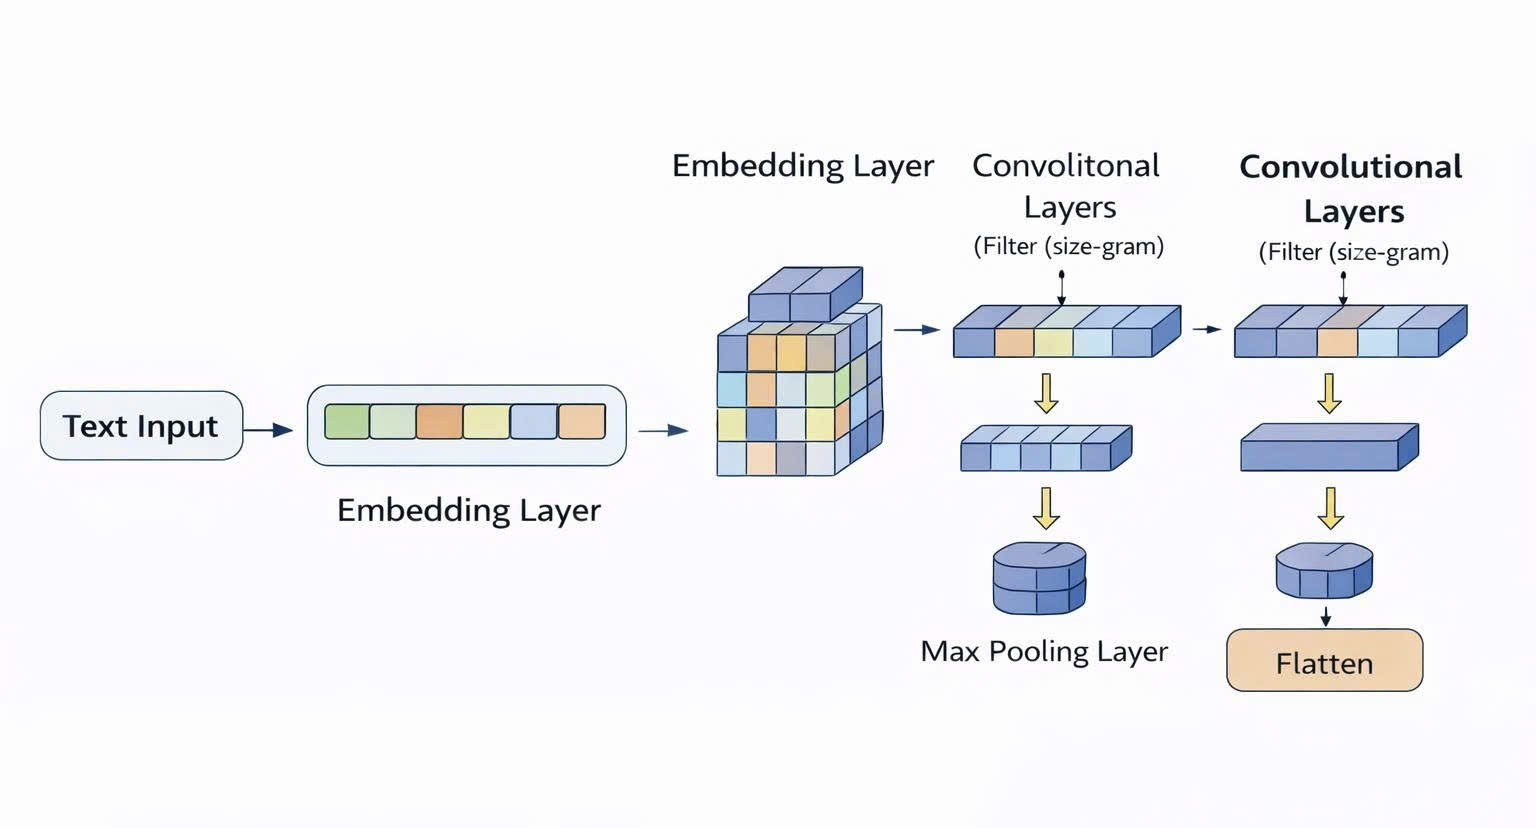
\includegraphics[width=0.75\textwidth]{images/CNN text model.jpg}
    \caption{Kiến trúc CNN dùng để trích xuất đặc trưng văn bản.}
    \label{fig:cnn}
\end{figure}

\subsection{Mạng nơ-ron nhớ dài-ngắn (Long Short-Term Memory -- LSTM)}

Long Short-Term Memory (LSTM) là một biến thể của mạng nơ-ron hồi tiếp \textbf{Recurrent Neural Network (RNN)}, được thiết kế nhằm khắc phục hạn chế của RNN truyền thống trong việc xử lý các chuỗi dữ liệu dài. Cụ thể, LSTM giải quyết vấn đề \textbf{triệt tiêu đạo hàm (vanishing gradient)}, giúp mô hình có khả năng ghi nhớ các phụ thuộc dài hạn trong dữ liệu tuần tự.

Trong xử lý ngôn ngữ tự nhiên, LSTM đặc biệt phù hợp cho các nhiệm vụ liên quan đến chuỗi văn bản, bởi mô hình có thể \textbf{ghi nhớ ngữ cảnh của các từ xuất hiện trước đó trong câu}. Điều này cho phép LSTM hiểu rõ hơn mối quan hệ giữa các từ và ý nghĩa tổng thể của câu.

Cơ chế hoạt động của LSTM dựa trên hệ thống \textbf{các cổng điều khiển (gating mechanism)} bao gồm:

\begin{itemize}
    \item \textbf{Input gate (cổng vào):} quyết định lượng thông tin mới được đưa vào bộ nhớ.
    \item \textbf{Forget gate (cổng quên):} xác định thông tin nào trong bộ nhớ cũ cần được loại bỏ.
    \item \textbf{Output gate (cổng ra):} quyết định phần thông tin nào sẽ được sử dụng làm đầu ra của mô hình.
\end{itemize}

Các cổng này phối hợp với \textbf{tế bào bộ nhớ (memory cell)} để kiểm soát luồng thông tin trong mạng, giúp LSTM có thể học và ghi nhớ các quan hệ ngữ nghĩa dài hạn trong câu hoặc đoạn văn bản.

\subsection{LSTM hai chiều (Bidirectional LSTM -- BiLSTM)}

Bidirectional LSTM (BiLSTM) là một mở rộng quan trọng của kiến trúc LSTM. Trong khi LSTM truyền thống chỉ xử lý chuỗi dữ liệu theo \textbf{một hướng từ trái sang phải}, BiLSTM xử lý dữ liệu theo \textbf{hai hướng đồng thời}:

\begin{itemize}
    \item hướng tiến (\textit{forward}): từ đầu câu đến cuối câu
    \item hướng lùi (\textit{backward}): từ cuối câu về đầu câu
\end{itemize}

Nhờ cơ chế này, BiLSTM có khả năng khai thác thông tin ngữ cảnh từ \textbf{cả hai phía của câu}, giúp mô hình hiểu đầy đủ hơn ý nghĩa của từng từ trong văn bản.

Điều này đặc biệt quan trọng trong bài toán phân tích cảm xúc, bởi ý nghĩa của một từ thường phụ thuộc vào các từ xung quanh. Ví dụ, các từ phủ định như ``không'', ``chưa'', ``chẳng'' có thể làm thay đổi hoàn toàn cực tính cảm xúc của từ đứng sau.

Nhờ khả năng nắm bắt tốt các mối quan hệ ngữ nghĩa và ngữ cảnh phức tạp, BiLSTM đã trở thành một trong những kiến trúc học sâu phổ biến và hiệu quả trong nhiều bài toán xử lý ngôn ngữ tự nhiên, bao gồm \textbf{phân tích cảm xúc, phân loại văn bản và nhận dạng thực thể}. Kiến trúc chi tiết của BiLSTM được minh họa trong Hình \ref{fig:bilstm}.

\begin{figure}[h]
    \centering
    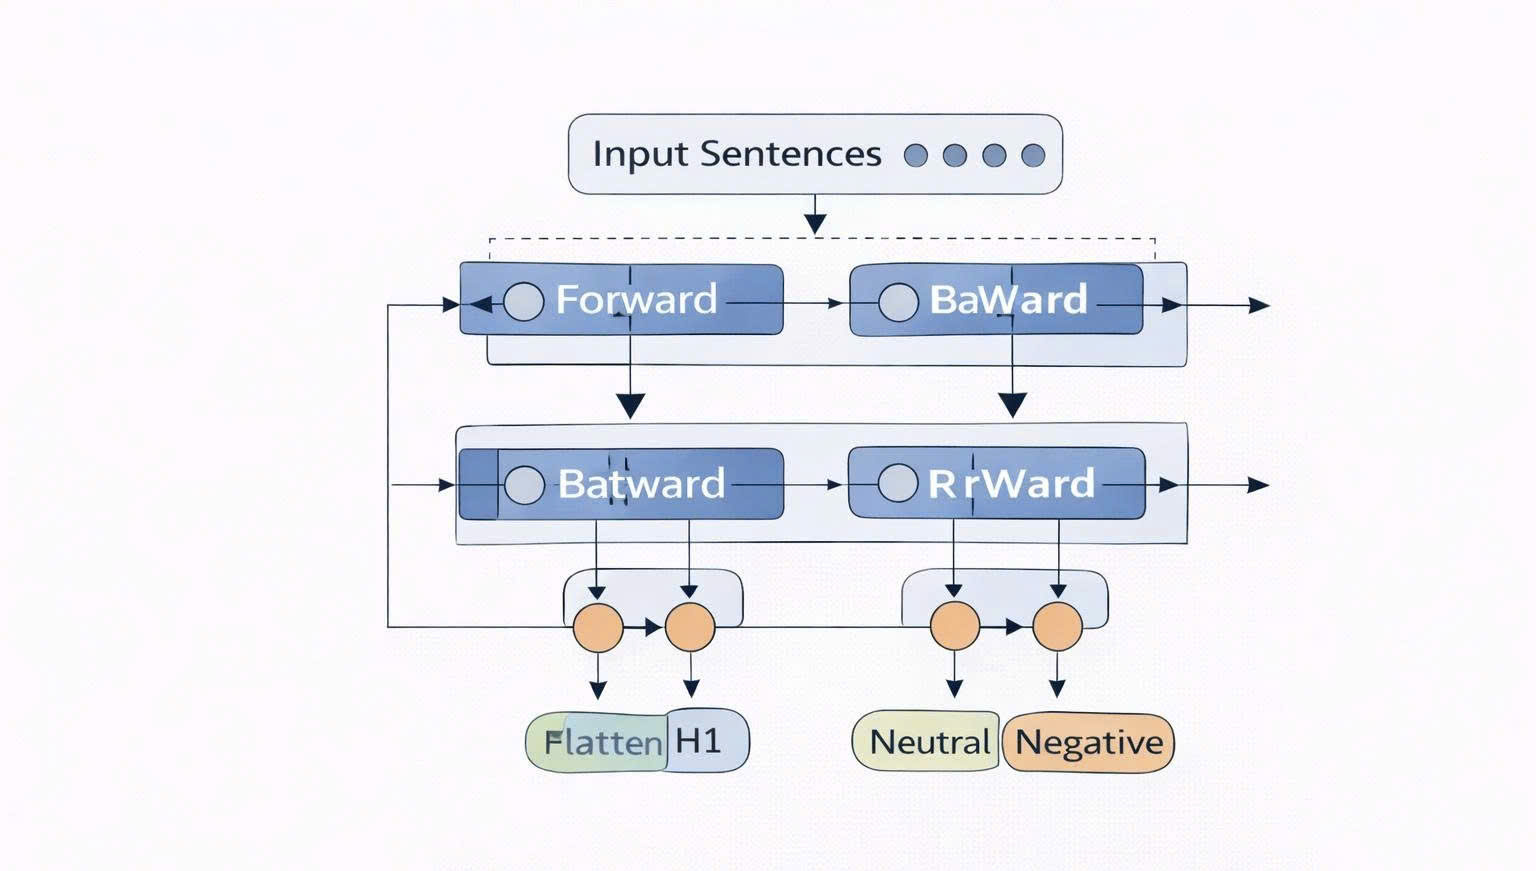
\includegraphics[width=0.75\textwidth]{images/BiLSTM architecture.jpg}
    \caption{Kiến trúc BiLSTM cho mô hình hóa ngữ cảnh hai chiều.}
    \label{fig:bilstm}
\end{figure}

\section{Các mô hình ngôn ngữ tiền huấn luyện và mô hình đề xuất dựa trên PhoBERT}

Sự phát triển của các \textbf{mô hình ngôn ngữ tiền huấn luyện (Pre-trained Language Models)} dựa trên kiến trúc Transformer đã tạo ra bước tiến lớn trong lĩnh vực xử lý ngôn ngữ tự nhiên. Nhờ cơ chế \textbf{Self-Attention}, các mô hình này có khả năng học được các phụ thuộc ngữ cảnh xa trong văn bản và xử lý dữ liệu hiệu quả hơn so với các mô hình RNN truyền thống.

Trong phân tích cảm xúc, các mô hình Transformer cho phép biểu diễn văn bản trong không gian ngữ nghĩa sâu, từ đó cải thiện đáng kể hiệu năng của hệ thống phân loại.

\subsection{Mô hình PhoBERT}

PhoBERT là một mô hình ngôn ngữ tiền huấn luyện được phát triển dành riêng cho tiếng Việt, dựa trên kiến trúc \textbf{RoBERTa}, một phiên bản cải tiến của BERT. Mô hình được huấn luyện trên một kho dữ liệu tiếng Việt rất lớn, bao gồm dữ liệu từ Wikipedia, báo chí và nhiều nguồn văn bản khác.

Trong quá trình huấn luyện, PhoBERT sử dụng phương pháp \textbf{Byte Pair Encoding (BPE)} để xử lý từ vựng và kết hợp với công cụ \textbf{RDRSegmenter} trong thư viện VnCoreNLP để thực hiện tách từ tiếng Việt. Nhờ đó, mô hình có thể học được các biểu diễn ngữ nghĩa phong phú và phù hợp với đặc trưng của ngôn ngữ tiếng Việt.

Các ưu điểm chính của PhoBERT bao gồm:

\begin{itemize}
    \item Khả năng hiểu \textbf{ngữ cảnh hai chiều} của câu
    \item Học được \textbf{biểu diễn ngữ nghĩa sâu} của văn bản
    \item Phù hợp với đặc trưng ngôn ngữ tiếng Việt
\end{itemize}

Trong các bài toán xử lý ngôn ngữ tự nhiên, PhoBERT thường được sử dụng như một \textbf{bộ trích xuất đặc trưng ngữ nghĩa} hoặc được \textbf{fine-tune trực tiếp} để thực hiện các nhiệm vụ như phân loại văn bản, phân tích cảm xúc hoặc nhận dạng thực thể.

\subsection{Mô hình lai PhoBERT--CNN--LSTM}

Để tận dụng ưu điểm của nhiều kiến trúc khác nhau, nghiên cứu này đề xuất sử dụng \textbf{mô hình lai PhoBERT--CNN--LSTM} cho bài toán phân tích cảm xúc.

Trong kiến trúc này, mỗi thành phần đảm nhiệm một vai trò khác nhau:

\begin{itemize}
    \item \textbf{PhoBERT}: đóng vai trò bộ mã hóa ngữ nghĩa, trích xuất các đặc trưng ngữ cảnh sâu từ văn bản.
    \item \textbf{CNN}: phát hiện các đặc trưng cục bộ trong câu, chẳng hạn như các cụm từ mang sắc thái cảm xúc mạnh.
    \item \textbf{LSTM/BiLSTM}: mô hình hóa quan hệ tuần tự giữa các từ và nắm bắt các phụ thuộc dài hạn trong câu.
\end{itemize}

Sự kết hợp này giúp mô hình vừa hiểu được \textbf{ngữ cảnh toàn cục của văn bản}, vừa phát hiện được \textbf{các đặc trưng cảm xúc cục bộ} và \textbf{quan hệ ngữ nghĩa theo chuỗi}. Nhờ đó, mô hình có khả năng nhận diện cảm xúc hiệu quả hơn, đặc biệt đối với các \textbf{bình luận ngắn và dữ liệu mạng xã hội tiếng Việt} vốn thường chứa nhiều từ lóng, viết tắt và cấu trúc ngôn ngữ không chuẩn. Kiến trúc chi tiết của mô hình đề xuất được minh họa trong Hình \ref{fig:phobert-cnn-lstm}.

\begin{figure}[h]
    \centering
    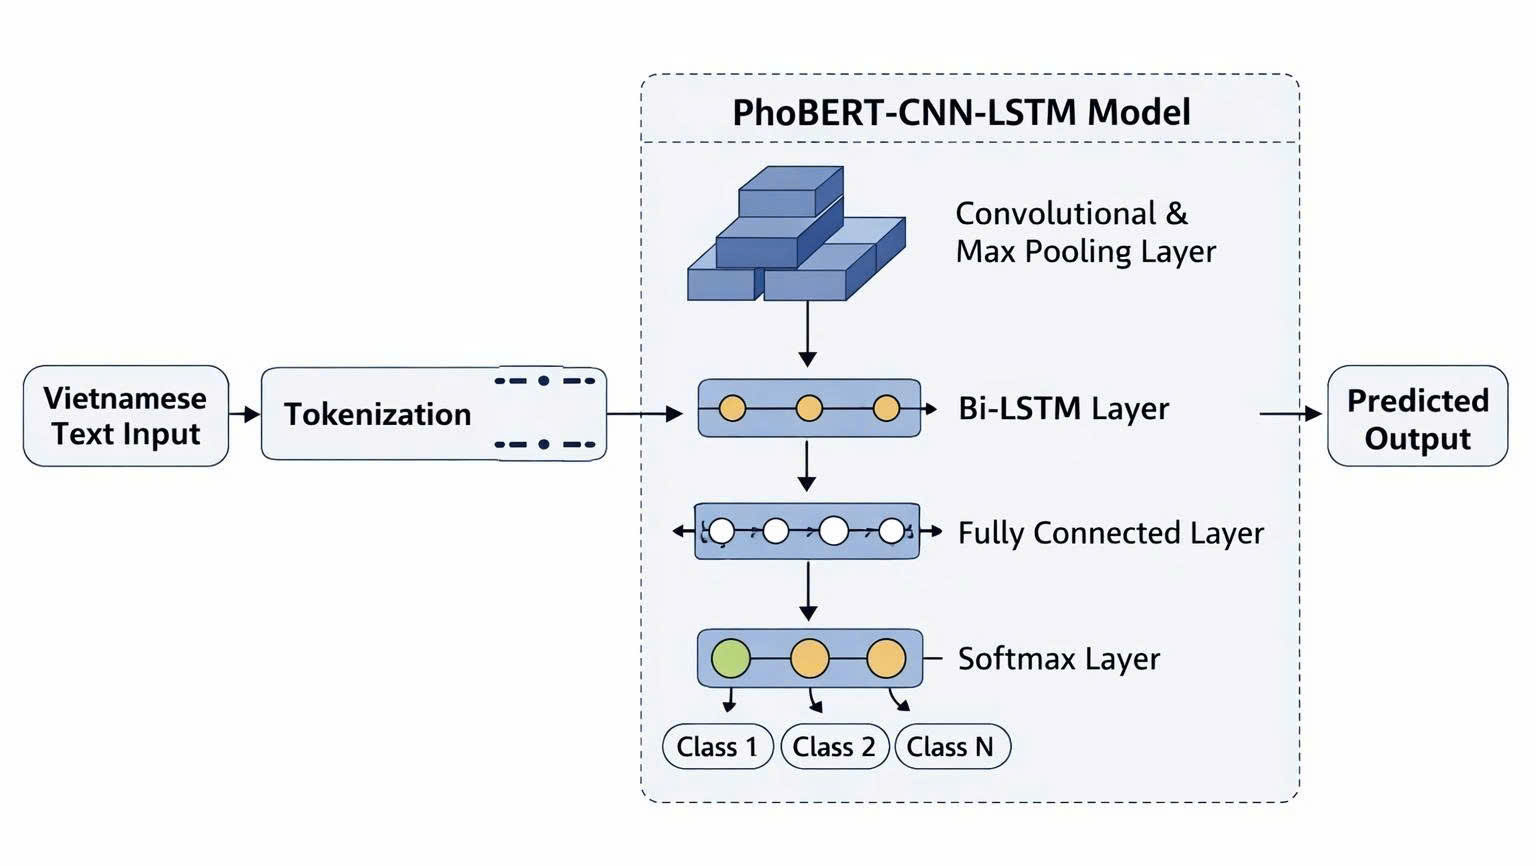
\includegraphics[width=0.75\textwidth]{images/PhoBERT-CNN-LSTM architecture.jpg}
    \caption{Kiến trúc mô hình PhoBERT-CNN-LSTM được đề xuất.}
    \label{fig:phobert-cnn-lstm}
\end{figure}

\section{Kiến trúc tổng thể của hệ thống}

Hệ thống phân tích cảm xúc được xây dựng theo kiến trúc gồm các thành phần chính sau:

\begin{enumerate}
    \item \textbf{Thu thập dữ liệu}
    \begin{itemize}
        \item Lấy dữ liệu từ các bộ dữ liệu công khai.
    \end{itemize}
    \item \textbf{Tiền xử lý dữ liệu}
    \begin{itemize}
        \item Chuẩn hóa văn bản
        \item Tách từ tiếng Việt
        \item Xử lý emoji và từ viết tắt.
    \end{itemize}
    \item \textbf{Biểu diễn văn bản}
    \begin{itemize}
        \item TF-IDF cho mô hình học máy truyền thống
        \item Embedding từ PhoBERT cho mô hình học sâu.
    \end{itemize}
    \item \textbf{Huấn luyện mô hình}
    \begin{itemize}
        \item Huấn luyện các mô hình học máy và học sâu.
    \end{itemize}
    \item \textbf{Đánh giá mô hình}
    \begin{itemize}
        \item So sánh hiệu năng dựa trên các chỉ số đánh giá.
    \end{itemize}
\end{enumerate}

Kết quả của hệ thống là nhãn cảm xúc tương ứng với mỗi bình luận. Pipeline tổng thể của hệ thống được minh họa trong Hình \ref{fig:pipeline}.

\begin{figure}[h]
    \centering
    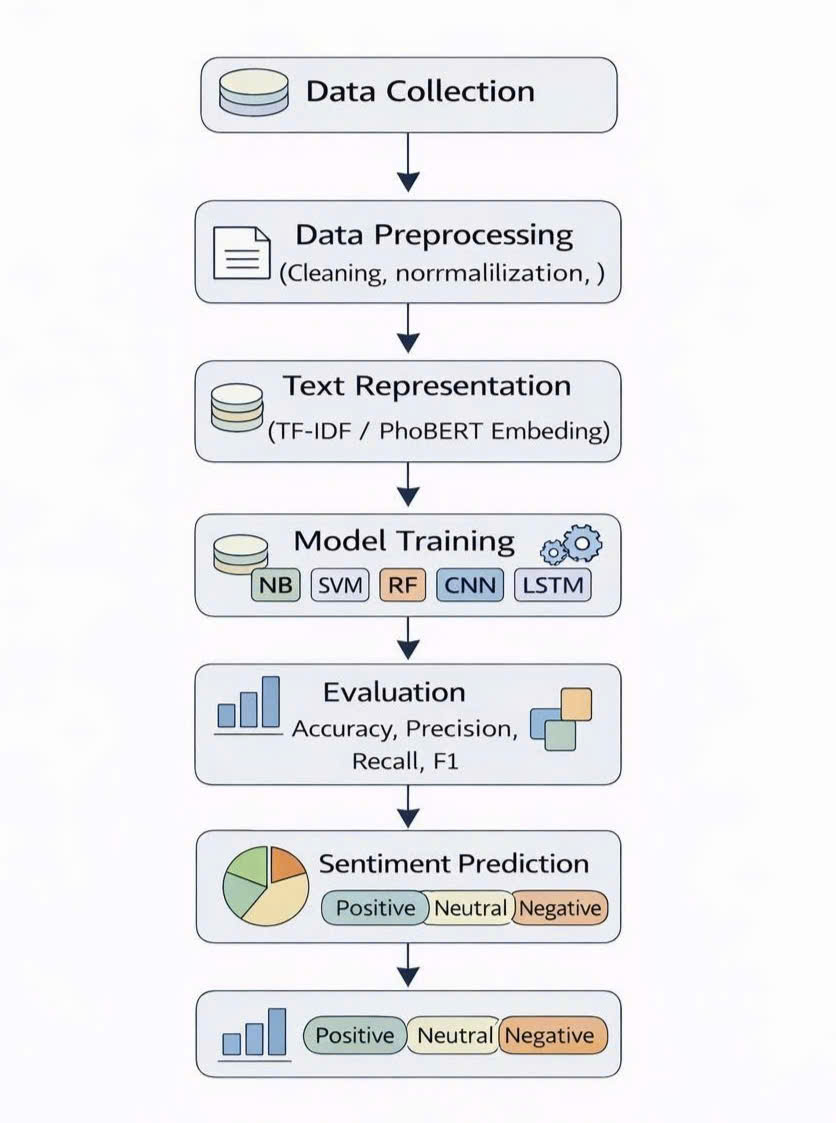
\includegraphics[width=0.9\textwidth]{images/Pipeline hệ thống.jpg}
    \caption{Pipeline tổng thể của hệ thống phân loại văn bản tiếng Việt.}
    \label{fig:pipeline}
\end{figure}

\section{Kết luận chương 2}

Chương 2 đã trình bày phương pháp nghiên cứu và các mô hình được sử dụng trong đề tài. Nội dung chương bao gồm quy trình tiền xử lý dữ liệu, các phương pháp biểu diễn văn bản, các mô hình học máy truyền thống và các mô hình học sâu hiện đại.

Đặc biệt, chương đã giới thiệu mô hình ngôn ngữ tiền huấn luyện PhoBERT và mô hình lai PhoBERT-CNN-LSTM được đề xuất nhằm cải thiện hiệu quả phân tích cảm xúc cho tiếng Việt. Những nội dung này là cơ sở để tiến hành thực nghiệm và đánh giá hiệu năng của các mô hình trong chương tiếp theo.

\chapter{Thực nghiệm và đánh giá}
\label{chap:chapter3}


\section{Mô tả tập dữ liệu và cách xây dựng tập huấn luyện}


Trong bài toán học máy có giám sát, chất lượng và quy mô của tập dữ liệu đóng vai trò quyết định đối với hiệu năng của mô hình. Đối với bài toán phân tích cảm xúc tiếng Việt, việc lựa chọn bộ dữ liệu phù hợp đòi hỏi phải xem xét nhiều yếu tố như độ tin cậy của nhãn gán, sự đa dạng của các lĩnh vực, mức độ nhiễu trong văn bản cũng như tính đại diện cho ngôn ngữ thực tế trên mạng xã hội. Mục này trình bày chi tiết tiêu chí lựa chọn dữ liệu, mô tả từng bộ dữ liệu được sử dụng, phân tích thống kê, đặc thù ngôn ngữ, quy trình tiền xử lý và phương pháp xây dựng tập huấn luyện.


\subsection{Tiêu chí lựa chọn và nguồn dữ liệu}


Việc lựa chọn dữ liệu nghiên cứu được thực hiện dựa trên một bộ tiêu chí chặt chẽ nhằm đảm bảo tính khoa học, khả năng tái lập và giá trị thực tiễn của kết quả nghiên cứu. Các tiêu chí chính bao gồm:


Thứ nhất, dữ liệu phải là tiếng Việt nguyên bản, được viết trực tiếp bởi người dùng Việt Nam trên các nền tảng trực tuyến. Yêu cầu này nhằm đảm bảo rằng các đặc trưng ngôn ngữ đặc thù như từ viết tắt, tiếng lóng, cách diễn đạt vùng miền và các hiện tượng ngôn ngữ mạng được bảo toàn tự nhiên, thay vì sử dụng dữ liệu dịch tự động từ ngôn ngữ khác vốn thường xuyên tạo ra các cấu trúc ngữ pháp không tự nhiên.


Thứ hai, dữ liệu phải được gán nhãn cảm xúc bởi con người (human-annotated) với hướng dẫn gán nhãn rõ ràng. Ưu tiên được dành cho các bộ dữ liệu đã qua quá trình kiểm tra chéo (inter-annotator agreement) để đảm bảo độ tin cậy của nhãn. Chỉ số kappa Cohen hoặc kappa Fleiss được sử dụng làm thước đo sự đồng thuận giữa các người gán nhãn, với ngưỡng chấp nhận tối thiểu là 0.6.


Thứ ba, dữ liệu phải có quy mô đủ lớn để huấn luyện các mô hình học sâu, đặc biệt là mô hình ngôn ngữ tiền huấn luyện PhoBERT yêu cầu một lượng dữ liệu đáng kể để fine-tune hiệu quả. Theo các nghiên cứu trước đây, số lượng mẫu tối thiểu cần thiết cho bài toán phân loại cảm xúc ba lớp với các mô hình Transformer là khoảng 5.000 mẫu trở lên.


Thứ tư, dữ liệu cần bao gồm nhiều lĩnh vực khác nhau để đánh giá khả năng tổng quát hóa của mô hình. Sự đa dạng về chủ đề giúp kiểm tra xem mô hình có thể nhận diện cảm xúc trong các ngữ cảnh khác nhau hay chỉ học được các mẫu đặc trưng của một lĩnh vực cụ thể.


Cuối cùng, dữ liệu phải được công khai trên các nền tảng dữ liệu mở (như Kaggle, GitHub, Zenodo) để đảm bảo tính tái lập của nghiên cứu. Điều này cho phép các nghiên cứu khác sử dụng cùng tập dữ liệu để so sánh kết quả một cách công bằng.


Dựa trên các tiêu chí trên, nghiên cứu đã khảo sát và đánh giá nhiều bộ dữ liệu tiếng Việt hiện có. Quá trình khảo sát bao gồm việc tìm kiếm trên nền tảng Kaggle với các từ khóa liên quan đến phân tích cảm xúc tiếng Việt, tham khảo danh sách dữ liệu NLP tiếng Việt từ kho lưu trữ Awesome Vietnamese NLP, và xem xét các bộ dữ liệu được đề cập trong các bài báo khoa học gần đây. Kết quả khảo sát cho thấy ba bộ dữ liệu đáp ứng tốt nhất các tiêu chí đặt ra bao gồm: UIT-ViSFD (Vietnamese Sentiment Food Dataset), bộ dữ liệu đánh giá sản phẩm thương mại điện tử trên Shopee, và bộ dữ liệu phản hồi của sinh viên về các khóa học trực tuyến.


\subsection{Mô tả chi tiết các bộ dữ liệu}


\subsubsection{a) Bộ dữ liệu UIT-ViSFD (Vietietnamese Sentiment Food Dataset)}


UIT-ViSFD là bộ dữ liệu phân tích cảm xúc tiếng Việt do nhóm nghiên cứu tại trường Đại học Công nghệ Thông tin (UIT), Đại học Quốc gia TP.HCM phát triển và công bố. Bộ dữ liệu này tập trung vào lĩnh vực dịch vụ ăn uống, bao gồm các bình luận và đánh giá về nhà hàng, quán ăn và món ăn được thu thập từ các nền tảng giao đồ ăn phổ biến tại Việt Nam như Foody và ShopeeFood (trước đây là Now).


Bộ dữ liệu UIT-ViSFD bao gồm tổng cộng 7.226 bình luận đã được gán nhãn. Mỗi bình luận được gán nhãn cảm xúc theo ba lớp: Positive (tích cực), Negative (tiêu cực) và Neutral (trung lập). Quá trình gán nhãn được thực hiện bởi ba người gán nhãn độc lập, sau đó tính toán chỉ số kappa Fleiss để đo lường mức độ đồng thuận. Các bình luận có sự không đồng thuận giữa các người gán nhãn được đưa vào vòng thảo luận thứ hai để đạt được sự nhất trí. Kết quả là chỉ số kappa đạt 0.78, cho thấy mức độ đồng thuận đáng kể (substantial agreement) theo thang đo Landis và Koch.


Đặc điểm nổi bật của UIT-ViSFD là sự phong phú về biểu đạt cảm xúc trong lĩnh vực ẩm thực. Các bình luận trong bộ dữ liệu phản ánh nhiều khía cạnh khác nhau của trải nghiệm ăn uống, bao gồm chất lượng món ăn, thái độ phục vụ, không gian quán, thời gian chờ đợi, giá cả và bao bì đóng gói (đối với đơn hàng giao tận nơi). Sự đa dạng về khía cạnh này tạo điều kiện thuận lợi để đánh giá khả năng nhận diện cảm xúc của mô hình trên các chủ đề cụ thể trong cùng một lĩnh vực.


Về độ dài văn bản, bình luận trong UIT-ViSFD có độ dài trung bình khoảng 35 từ, với độ dài ngắn nhất là 3 từ và dài nhất là 245 từ. Khoảng 60\% bình luận có độ dài từ 15 đến 50 từ, phản ánh đặc điểm điển hình của các đánh giá trực tuyến ngắn gọn trên nền tảng di động. Phân bố này phù hợp với mục tiêu nghiên cứu về phân tích cảm xúc trên bình luận mạng xã hội.


\subsubsection{b) Bộ dữ liệu đánh giá sản phẩm thương mại điện tử (Shopee Reviews)}


Bộ dữ liệu đánh giá sản phẩm thương mại điện tử được thu thập từ nền tảng Shopee, một trong những sàn thương mại điện tử lớn nhất Việt Nam với hơn 70 triệu người dùng hoạt động. Dữ liệu bao gồm các bình luận và đánh giá sản phẩm từ nhiều danh mục khác nhau, bao gồm thời trang, điện tử, mỹ phẩm, đồ gia dụng và thực phẩm.


Bộ dữ liệu này bao gồm khoảng 15.800 bình luận đã gán nhãn cảm xúc. Việc gán nhãn được thực hiện theo phương pháp kết hợp giữa tự động và thủ công. Cụ thể, các bình luận được phân loại ban đầu dựa trên đánh giá sao (rating) của người dùng: bình luận kèm đánh giá 4-5 sao được gán nhãn Positive, đánh giá 1-2 sao được gán nhãn Negative, và đánh giá 3 sao được gán nhãn Neutral. Sau đó, một nhóm gồm năm người gán nhãn tiến hành kiểm tra và điều chỉnh nhãn cho các bình luận có sự mâu thuẫn giữa nội dung văn bản và số sao đánh giá, ví dụ các trường hợp người dùng cho 5 sao nhưng nội dung bình luận lại mang sắc thái tiêu cực hoặc mỉa mai.


Một đặc điểm đáng chú ý của bộ dữ liệu này là sự hiện diện đáng kể của các bình luận ngắn, không chuẩn hóa và sử dụng nhiều ngôn ngữ mạng. Khoảng 35\% bình luận có độ dài dưới 10 từ, bao gồm các biểu đạt ngắn gọn như "oke", "dep lam", "ship cham", "ko ung y", "sp binh thuong". Ngoài ra, bộ dữ liệu cũng chứa một lượng lớn từ viết tắt đặc trưng của thương mại điện tử như "sp" (sản phẩm), "ship" (giao hàng), "shop" (người bán), "admin" (quản trị viên), "lh" (liên hệ), và các biểu tượng cảm xúc (emoji) được sử dụng phổ biến để diễn tả mức độ hài lòng hoặc không hài lòng.


Về phân bố nhãn, bộ dữ liệu này có sự mất cân bằng đáng kể: lớp Positive chiếm tỷ lệ cao nhất (khoảng 52\%), theo sau là lớp Negative (khoảng 30\%) và lớp Neutral chỉ chiếm khoảng 18\%. Sự mất cân bằng này phản ánh xu hướng thực tế trên các nền tảng thương mại điện tử, nơi người dùng có xu hướng viết đánh giá khi có trải nghiệm tích cực hoặc tiêu cực mạnh, trong khi ít khi để lại đánh giá trung lập.


\subsubsection{c) Bộ dữ liệu phản hồi giáo dục (Student Feedback Dataset)}


Bộ dữ liệu phản hồi giáo dục bao gồm các bình luận và nhận xét của sinh viên về các khóa học trực tuyến và các môn học tại trường đại học. Dữ liệu được thu thập từ các nền tảng đánh giá giáo dục và diễn đàn sinh viên, bao gồm các bình luận về chất lượng giảng dạy, nội dung khóa học, cơ sở vật chất và dịch vụ hỗ trợ sinh viên.


Bộ dữ liệu này bao gồm khoảng 8.200 bình luận đã gán nhãn. Việc gán nhãn được thực hiện bởi hai nhóm người gán nhãn độc lập, mỗi nhóm gồm ba người, với quy trình hai vòng tương tự như UIT-ViSFD. Điểm đặc biệt của bộ dữ liệu này là các bình luận thường mang tính chất phân tích và dài hơn so với hai bộ dữ liệu còn lại, với độ dài trung bình khoảng 45 từ. Các bình luận trong lĩnh vực giáo dục thường có cấu trúc ngữ pháp phức tạp hơn, sử dụng nhiều thuật ngữ chuyên ngành và thường chứa đan xen nhiều khía cạnh trong cùng một bình luận, ví dụ: "Giảng viên rất nhiệt tình nhưng tài liệu thì outdated quá, nên mình chỉ đánh giá trung bình."


Phân bố nhãn trong bộ dữ liệu giáo dục tương đối cân bằng hơn so với bộ dữ liệu thương mại điện tử: lớp Positive chiếm khoảng 42\%, lớp Negative chiếm khoảng 33\% và lớp Neutral chiếm khoảng 25\%. Sự cân bằng tốt hơn này có thể được giải thích bởi đặc thù của lĩnh vực giáo dục, nơi sinh viên có xu hướng đưa ra nhận xét đa chiều hơn, bao gồm cả điểm tích cực và tiêu cực trong cùng một đánh giá.


\subsection{Quá trình chuẩn bị và gán nhãn dữ liệu}


Việc xây dựng tập dữ liệu chất lượng cao là một trong những công đoạn đòi hỏi nhiều công sức và thời gian nhất trong toàn bộ nghiên cứu. Mục này trình bày chi tiết quá trình chuẩn bị, làm sạch và gán nhãn dữ liệu mà nhóm nghiên cứu đã thực hiện.


a) Thu thập và tổng hợp dữ liệu


Nghiên cứu thu thập dữ liệu từ ba nguồn khác nhau gồm UIT-ViSFD (7.226 mẫu), Shopee Reviews (15.800 mẫu) và Student Feedback (8.200 mẫu), mang về tổng cộng 31.226 bình luận tiếng Việt. Quá trình tải về, kiểm tra tính toàn vẹn và đồng nhất định dạng dữ liệu được thực hiện thủ công, đảm bảo mỗi bộ dữ liệu có cấu trúc nhất quán với các trường thông tin cần thiết: nội dung bình luận, nhãn cảm xúc và nguồn dữ liệu.


b) Làm sạch và tiền kiểm tra dữ liệu


Sau khi tổng hợp, nhóm nghiên cứu tiến hành kiểm tra và làm sạch dữ liệu qua nhiều bước: loại bỏ 412 bình luận trùng lặp phát hiện được bằng thuật toán so khớp chuỗi; loại bỏ 187 bình luận chỉ chứa emoji hoặc ký tự đặc biệt không có nội dung văn bản; loại bỏ 95 bình luận có độ dài dưới 2 từ không mang ý nghĩa cảm xúc rõ ràng (ví dụ: "ok", "hihi", "..."). Ngoài ra, 63 bình luận chứa nội dung không phải tiếng Việt hoặc đan xen ngôn ngữ khác cũng được loại bỏ. Tổng cộng, sau bước làm sạch, tập dữ liệu giữ lại 31.226 mẫu đạt tiêu chất lượng.


c) Kiểm tra và chuẩn hóa nhãn cảm xúc


Do dữ liệu được gom từ ba nguồn khác nhau với các bộ nhãn và phương pháp gán nhãn không hoàn toàn đồng nhất, nhóm nghiên cứu tiến hành chuẩn hóa hệ thống nhãn về ba lớp thống nhất: Positive (tích cực), Negative (tiêu cực) và Neutral (trung tính). Cụ thể, bộ dữ liệu UIT-ViSFD sử dụng sẵn ba nhãn tương thích; bộ Shopee Reviews ban đầu có 5 mức đánh giá (1–5 sao) được quy đổi về ba lớp theo nguyên tắc: 1–2 sao → Negative, 3 sao → Neutral, 4–5 sao → Positive; bộ Student Feedback đã có sẵn ba lớp nhãn tương ứng.


Để đảm bảo chất lượng gán nhãn, nhóm nghiên cứu tiến hành kiểm tra ngẫu nhiên 2.000 mẫu (khoảng 6,4\% tổng dữ liệu) bằng phương pháp đánh giá chéo giữa hai thành viên. Kết quả cho thấy tỷ lệ đồng thuận (inter-annotator agreement) đạt 87,3\%, với chỉ số Cohen's Kappa là 0,81, cho thấy mức độ đồng thuận tốt. Các mẫu gây tranh cãi (253 mẫu, chiếm 12,7\%) được thảo luận lại và gán nhãn lại theo sự đồng thuận của cả nhóm.


d) Công sức và thời gian thực hiện


Toàn bộ quá trình thu thập, làm sạch và kiểm tra nhãn dữ liệu kéo dài khoảng hai tuần. Trong đó, việc tải và đồng nhất dữ liệu mất khoảng hai ngày; quá trình làm sạch và loại bỏ mẫu lỗi mất khoảng bốn ngày; việc kiểm tra chéo 2.000 mẫu và xử lý các mẫu tranh cãi tiêu tốn khoảng tám ngày; thời gian còn lại dành cho thống kê, phân tích và lập báo cáo. Tổng số giờ làm việc ước tính khoảng 100 giờ, trong đó phần lớn thời gian dành cho việc đọc và đánh giá thủ công từng bình luận.


Công đoạn tốn nhiều công sức nhất là bước kiểm tra chéo nhãn, do yêu cầu cả hai thành viên phải độc lập đọc và đánh giá từng bình luận, sau đó đối chiếu kết quả với nhau. Đặc biệt, các bình luận thuộc nhóm Neutral hoặc chứa mỉa mai thường gây khó khăn nhất cho người gán nhãn, đòi hỏi sự thảo luận và phân tích ngữ cảnh kỹ lưỡng.


\subsection{Thống kê và phân tích phân bố dữ liệu tổng hợp}


Sau khi thu thập ba bộ dữ liệu, nghiên cứu tiến hành gộp dữ liệu thành một tập tổng hợp thống nhất. Trước khi gộp, các bước kiểm tra chất lượng được thực hiện bao gồm: loại bỏ các bình luận trùng lặp, loại bỏ bình luận chỉ chứa emoji hoặc ký tự đặc biệt không có nội dung văn bản, và loại bỏ các bình luận có độ dài dưới 2 từ không mang ý nghĩa cảm xúc rõ ràng (ví dụ: "ok", "hihi").


Kết quả sau khi gộp và làm sạch sơ bộ, tập dữ liệu tổng hợp bao gồm 31.226 bình luận đã gán nhãn. Phân bố cụ thể theo từng bộ dữ liệu và nhãn cảm xúc được trình bày chi tiết trong Bảng 3.1.


\begin{table}[h]
\centering
\caption{Phân bố dữ liệu theo nguồn và nhãn cảm xúc}
\begin{tabular}{|l|c|c|c|c|}
\hline
\textbf{Bộ dữ liệu} & \textbf{Tổng số mẫu} & \textbf{Positive} & \textbf{Negative} & \textbf{Neutral} \\
\hline
UIT-ViSFD (Ẩm thực) & 7.226 (100\%) & 2.891 (40,0\%) & 2.529 (35,0\%) & 1.806 (25,0\%) \\
\hline
Shopee Reviews (TMĐT) & 15.800 (100\%) & 8.216 (52,0\%) & 4.740 (30,0\%) & 2.844 (18,0\%) \\
\hline
Student Feedback (Giáo dục) & 8.200 (100\%) & 3.444 (42,0\%) & 2.706 (33,0\%) & 2.050 (25,0\%) \\
\hline
Tổng cộng & 31.226 (100\%) & 14.551 (46,6\%) & 9.975 (32,0\%) & 6.700 (21,4\%) \\
\hline
\end{tabular}
\normalsize
\end{table}




Có thể nhận thấy tập dữ liệu tổng hợp có sự mất cân bằng nhẹ giữa các nhãn, với tỷ lệ Positive gần gấp đôi Neutral. Để giải quyết vấn đề này, nghiên cứu xem xét hai phương án: (1) sử dụng trọng số lớp (class weights) trong hàm mất mát để bù đắp sự mất cân bằng, và (2) áp dụng kỹ thuật tăng cường dữ liệu (data augmentation) như dịch ngược (back-translation) và thay thế từ đồng nghĩa cho lớp thiểu số. Kết quả cho thấy việc sử dụng trọng số lớp mang lại hiệu quả ổn định hơn so với tăng cường dữ liệu, do các phương pháp tăng cường dữ liệu trên tiếng Việt vẫn còn hạn chế về chất lượng.


Bên cạnh phân bố nhãn, nghiên cứu cũng tiến hành phân tích đặc trưng độ dài văn bản trong tập dữ liệu. Thống kê chi tiết được trình bày trong Bảng 3.2.


\begin{table}[h]
\centering
\caption{Thống kê độ dài văn bản trong tập dữ liệu (đơn vị: từ)}
\begin{tabular}{|l|c|}
\hline
\textbf{Chỉ số thống kê} & \textbf{Giá trị} \\
\hline
Độ dài tối thiểu & 2 từ \\
\hline
Độ dài tối đa & 312 từ \\
\hline
Độ dài trung bình (mean) & 38,7 từ \\
\hline
Độ dài trung vị (median) & 28 từ \\
\hline
Độ lệch chuẩn (std) & 31,4 từ \\
\hline
Phân vị thứ 25 (Q1) & 14 từ \\
\hline
Phân vị thứ 75 (Q3) & 52 từ \\
\hline
\end{tabular}
\normalsize
\end{table}




Phân tích cho thấy phân bố độ dài văn bản có dạng lệch phải (right-skewed), với phần lớn bình luận tập trung ở khoảng 10 đến 50 từ. Khoảng 15\% bình luận có độ dài dưới 5 từ, chủ yếu là các phản hồi ngắn gọn trên nền tảng thương mại điện tử. Ngược lại, khoảng 8\% bình luận có độ dài vượt quá 100 từ, phần lớn đến từ bộ dữ liệu phản hồi giáo dục. Sự đa dạng về độ dài này đòi hỏi mô hình phải có khả năng xử lý hiệu quả cả bình luận ngắn (thiếu ngữ cảnh) và bình luận dài (chứa nhiều thông tin và có thể đan xen nhiều cảm xúc).


Nghiên cứu cũng phân tích kích thước từ vựng trong tập dữ liệu. Trước tiền xử lý, tập dữ liệu chứa 42.568 từ vựng duy nhất. Sau khi tách từ bằng VnCoreNLP, số lượng từ ghép (compound words) được tạo ra là khoảng 8.900 từ, chẳng hạn "sinh\_viên", "chất\_lượng", "thương\_mại\_điện\_tử". Kích thước từ vựng lớn cùng với sự hiện diện của nhiều từ viết tắt, từ lóng và lỗi chính tả đặt ra thách thức đáng kể cho việc xây dựng mô hình phân loại.


\subsection{Phân tích đặc thù ngôn ngữ trong dữ liệu}


Để hiểu rõ hơn về các thách thức trong việc xử lý dữ liệu tiếng Việt, nghiên cứu tiến hành phân tích chi tiết các hiện tượng ngôn ngữ đặc thù xuất hiện trong tập dữ liệu. Phân tích được thực hiện bằng cách lấy mẫu ngẫu nhiên 2.000 bình luận từ mỗi bộ dữ liệu và gán nhãn thủ công các hiện tượng ngôn ngữ xuất hiện. Kết quả phân tích được tổng hợp trong Bảng 3.3.


\begin{table}[h]
\centering
\caption{Tỷ lệ xuất hiện các hiện tượng ngôn ngữ đặc thù trong tập dữ liệu}
\begin{tabular}{|l|c|c|}
\hline
\textbf{Hiện tượng ngôn ngữ} & \textbf{Tỷ lệ} & \textbf{Ví dụ} \\
\hline
Từ viết tắt & 67,3\% & ko/không, j/gì, k/không, mn/mọi người \\
\hline
Tiếng lóng \& ngôn ngữ mạng & 43,8\% & xịn xò, chán phèo, đỉnh chóp \\
\hline
Emoji \& biểu tượng cảm xúc & 52,1\% & [smile], [heart], [thumbs-down], [angry], [laugh], [disgust] \\
\hline
Lỗi chính tả & 28,5\% & hjhj, jì, ngta, rùi, wen \\
\hline
Ký tự đặc biệt \& URL & 19,4\% & đường dẫn, mã HTML \\
\hline
Đan xen nhiều cảm xúc & 14,2\% & "Sản phẩm tốt nhưng phục vụ quá tệ" \\
\hline
Từ vùng miền & 11,6\% & tui/mình, bữa/ngày, ngọt/xanh \\
\hline
Mỉa mai \& châm biếm & 8,7\% & "Giao hàng nhanh lắm, 2 tuần mới nhận" \\
\hline
\end{tabular}
\normalsize
\end{table}




Kết quả phân tích cho thấy từ viết tắt là hiện tượng phổ biến nhất với 67,3\% bình luận chứa ít nhất một từ viết tắt. Điều này phản ánh thói quen giao tiếp nhanh trên các nền tảng trực tuyến của người dùng Việt Nam. Đặc biệt, trong môi trường thương mại điện tử, người dùng thường viết ngắn gọn để tiết kiệm thời gian, dẫn đến sự xuất hiện của nhiều biến thể viết tắt cho cùng một từ, ví dụ: "không" có thể được viết dưới dạng "ko", "k", "hok", "hem", "ks", "kh", "kg".


Emoji xuất hiện trong hơn một nửa số bình luận, đóng vai trò quan trọng trong việc thể hiện cảm xúc. Phân tích chi tiết cho thấy các emoji thường được sử dụng tương quan với nhãn cảm xúc: emoji [smile], [heart], [thumbs-up], [love] thường xuất hiện trong bình luận Positive; emoji [thumbs-down], [angry], [disgust], [frustrated] thường trong bình luận Negative; emoji [neutral-face], [thinking] thường trong bình luận Neutral. Tuy nhiên, có một số ngoại lệ đáng chú ý, ví dụ emoji [laugh] có thể xuất hiện trong cả bình luận Positive (biểu thị sự vui vẻ) và Negative (biểu thị sự bất lực, mỉa mai).


Hiện tượng mỉa mai, dù chỉ chiếm 8,7\%, lại là một trong những nguyên nhân chính gây ra sai sót phân loại. Các bình luận mỉa mai thường sử dụng từ ngữ mang nghĩa tích cực nhưng trong ngữ cảnh tiêu cực, ví dụ: "Sản phẩm tuyệt vời lắm, dùng 1 ngày đã hỏng", "Ship nhanh như rùa bò vậy". Nhận diện hiện tượng này đòi hỏi mô hình phải có khả năng hiểu ngữ cảnh sâu, không chỉ dựa vào từ vựng đơn lẻ.


\subsection{Quy trình tiền xử lý dữ liệu chi tiết}


Dựa trên phân tích đặc thù ngôn ngữ ở mục 3.1.4, nghiên cứu xây dựng một quy trình tiền xử lý dữ liệu chuyên biệt cho tiếng Việt gồm 7 bước tuần tự. Mỗi bước được thiết kế để giải quyết một loại nhiễu cụ thể trong dữ liệu mạng xã hội, đồng thời bảo toàn tối đa thông tin cảm xúc có giá trị cho mô hình phân loại.


Bước 1: Chuẩn hóa ký tự Unicode. Tiếng Việt sử dụng nhiều ký tự đặc biệt có thể được biểu diễn dưới nhiều dạng Unicode khác nhau. Ví dụ, chữ "ạ" có thể được mã hóa dưới dạng tổ hợp (NFD) hoặc dạng tiền tổ hợp (NFC). Sự không nhất quán trong mã hóa có thể khiến cùng một từ được biểu diễn khác nhau, làm tăng kích thước từ vựng và giảm hiệu quả mô hình. Nghiên cứu sử dụng thư viện unicodedata của Python để chuẩn hóa toàn bộ văn bản về dạng NFC (Normalization Form C), đảm bảo mỗi ký tự tiếng Việt chỉ có một biểu diễn duy nhất.


Bước 2: Chuẩn hóa văn bản cơ bản. Bước này bao gồm việc chuyển toàn bộ văn bản sang chữ thường để giảm kích thước từ vựng (ví dụ: "Tốt" và "tốt" được coi là cùng một từ), chuẩn hóa khoảng trắng thừa (nhiều khoảng trắng liên tiếp được thay bằng một khoảng trắng duy nhất), và loại bỏ các ký tự điều khiển (control characters) không hiển thị nhưng có thể gây nhiễu trong quá trình tokenization.


Bước 3: Xử lý URL, email và số điện thoại. Các bình luận trực tuyến thường chứa đường dẫn URL, địa chỉ email hoặc số điện thoại không mang thông tin cảm xúc. Nghiên cứu sử dụng biểu thức chính quy (regular expression) để nhận diện và thay thế các thành phần này bằng các token đặc biệt tương ứng: [URL], [EMAIL], [PHONE]. Việc thay thế thay vì loại bỏ hoàn toàn giúp mô hình biết rằng tại vị trí đó từng có thông tin liên quan đến liên kết hoặc thông tin liên lạc, có thể ảnh hưởng đến ngữ cảnh cảm xúc.


Bước 4: Chuyển đổi emoji thành văn bản. Khác với nhiều nghiên cứu trước đây đơn giản loại bỏ emoji, nghiên cứu này chuyển đổi emoji thành các từ mô tả cảm xúc tương ứng bằng cách sử dụng thư viện emoji (Python) kết hợp với một từ điển ánh xạ thủ công được xây dựng dành riêng cho ngữ cảnh tiếng Việt. Ví dụ: [smile] được chuyển thành "cười\_hài\_lòng", [heart] thành "yêu\_thích", [thumbs-down] thành "không\_hài\_lòng", [angry] thành "tức\_giận", [laugh] thành "cười\_ra\_nước\_mắt". Cách tiếp cận này giúp bảo toàn thông tin cảm xúc từ emoji dưới dạng văn bản mà mô hình có thể học được.


Bước 5: Chuẩn hóa từ viết tắt và tiếng lóng. Đây là bước quan trọng nhất trong quy trình tiền xử lý cho tiếng Việt. Nghiên cứu xây dựng một từ điển chuẩn hóa gồm 438 mục từ, bao gồm các từ viết tắt phổ biến, tiếng lóng mạng và các biến thể viết tắt. Từ điển được xây dựng bằng cách kết hợp hai nguồn: (1) các từ điển tiếng lóng và từ viết tắt tiếng Việt có sẵn từ các nghiên cứu trước, và (2) phân tích tần suất từ vựng trong tập dữ liệu huấn luyện để phát hiện và thêm các từ viết tắt mới. Một số ví dụ ánh xạ tiêu biểu bao gồm: "ko" hoặc "k" hoặc "hok" hoặc "hem" hoặc "ks" được chuẩn hóa thành "không"; "j" hoặc "jì" được chuẩn hóa thành "gì"; "dc" hoặc "đc" được chuẩn hóa thành "được"; "vs" được chuẩn hóa thành "với"; "mn" được chuẩn hóa thành "mọi người"; "ak" hoặc "á" được chuẩn hóa thành "ạ".


Để xử lý các trường hợp từ viết tắt không có trong từ điển, nghiên cứu áp dụng kỹ thuật khoảng cách chỉnh sửa (edit distance) để tìm từ gần nhất trong từ điển chuẩn. Ví dụ, "hok" có khoảng cách Levenshtein bằng 1 so với "không" sau khi loại bỏ ký tự "h" và thêm "kh" ở đầu. Tuy nhiên, phương pháp này chỉ được áp dụng khi khoảng cách chỉnh sửa nhỏ hơn hoặc bằng 2 để tránh chuẩn hóa sai.


Bước 6: Tách từ tiếng Việt (Word Segmentation). Như đã trình bày ở Chương 1, tiếng Việt là ngôn ngữ đơn lập trong đó khoảng trắng dùng để phân tách âm tiết chứ không phải từ. Do đó, bước tách từ đóng vai trò quan trọng trong việc xác định ranh giới từ tiếng Việt. Nghiên cứu sử dụng công cụ RDRSegmenter từ thư viện VnCoreNLP, được đánh giá là một trong những công cụ tách từ tiếng Việt chính xác nhất với F1-score đạt 97.9\% trên tập dữ liệu benchmark. Kết quả tách từ nối các âm tiết thuộc cùng một từ bằng dấu gạch dưới, ví dụ: "chất lượng sản phẩm rất tốt" được chuyển thành "chất\_lượng sản\_phẩm rất tốt". Đối với mô hình PhoBERT, bước tách từ đặc biệt quan trọng vì bộ tokenizer của PhoBERT được thiết kế để hoạt động với văn bản đã được tách từ trước.


Bước 7: Loại bỏ từ dừng (Stopwords Removal). Từ dừng là các từ xuất hiện thường xuyên nhưng ít mang ý nghĩa phân biệt cảm xúc, ví dụ: "là", "và", "của", "một", "những", "đã", "sẽ". Nghiên cứu sử dụng danh sách từ dừng tiếng Việt từ thư viện VnCoreNLP, đồng thời tùy chỉnh danh sách này bằng cách loại bỏ một số từ có thể mang thông tin cảm xúc, ví dụ: từ "không" được giữ lại vì nó đóng vai trò quan trọng trong việc phủ định cảm xúc ("không tốt" vs. "tốt"). Danh sách từ dừng cuối cùng bao gồm 195 từ.


Để đánh giá tác động của quy trình tiền xử lý, nghiên cứu tiến hành thử nghiệm ablation study, trong đó từng bước tiền xử lý được loại bỏ lần lượt để đo lường mức độ ảnh hưởng của từng bước đến hiệu năng mô hình. Kết quả chi tiết sẽ được trình bày trong mục 3.5.


\subsection{Xây dựng tập huấn luyện, xác thực và kiểm thử}


Sau khi hoàn tất quy trình tiền xử lý, dữ liệu được chia thành ba tập con phục vụ cho các mục đích khác nhau: tập huấn luyện (train set) để tối ưu tham số mô hình, tập xác thực (validation set) để điều chỉnh siêu tham số và ngăn chặn quá khớp, và tập kiểm thử (test set) để đánh giá hiệu năng cuối cùng.


Tỷ lệ chia dữ liệu được thiết lập theo nguyên tắc phổ biến trong học máy: 80\% cho tập huấn luyện, 10\% cho tập xác thực và 10\% cho tập kiểm thử. Cụ thể, trên tổng số 31.226 mẫu, tập huấn luyện bao gồm 24.980 mẫu, tập xác thực gồm 3.123 mẫu và tập kiểm thử gồm 3.123 mẫu.


Một điểm quan trọng trong phương pháp chia dữ liệu là việc sử dụng phương pháp phân tầng (stratified split). Phương pháp này đảm bảo tỷ lệ phân bố các nhãn cảm xúc trong từng tập con tỷ lệ thuận với phân bố trong tập dữ liệu gốc. Điều này đặc biệt cần thiết do tập dữ liệu có sự mất cân bằng nhẹ giữa các lớp (Positive: 46.6\%, Negative: 32.0\%, Neutral: 21.4\%). Nếu chia ngẫu nhiên đơn thuần, có thể dẫn đến tình trạng một tập con bị thiếu một lớp cảm xúc nhất định hoặc có tỷ lệ phân bố khác biệt đáng kể so với tập gốc, làm sai lệch kết quả đánh giá.


Nghiên cứu sử dụng hàm train\_test\_split từ thư viện Scikit-learn với tham số stratify được thiết lập theo nhãn cảm xúc và random\_state = 42 để đảm bảo tính tái lập. Quá trình chia được thực hiện thành hai giai đoạn: đầu tiên, dữ liệu được chia thành tập huấn luyện (80\%) và tập tạm thời (20\%); sau đó, tập tạm thời được chia tiếp thành tập xác thực (50\%) và tập kiểm thử (50\%), tức mỗi tập chiếm 10\% tổng dữ liệu.


Phân bố chi tiết của các tập dữ liệu sau khi chia được trình bày trong Bảng 3.4.


\begin{table}[h]
\centering
\caption{Phân bố dữ liệu sau khi chia tập}
\begin{tabular}{|l|c|c|c|c|}
\hline
\textbf{Tập dữ liệu} & \textbf{Số mẫu} & \textbf{Positive} & \textbf{Negative} & \textbf{Neutral} \\
\hline
Huấn luyện (80\%) & 24.980 & 11.640 (46,6\%) & 7.980 (32,0\%) & 5.360 (21,4\%) \\
\hline
Xác thực (10\%) & 3.123 & 1.455 (46,6\%) & 998 (32,0\%) & 670 (21,4\%) \\
\hline
Kiểm thử (10\%) & 3.123 & 1.456 (46,6\%) & 997 (32,0\%) & 670 (21,4\%) \\
\hline
\end{tabular}
\end{table}




Ngoài ra, để đảm bảo tính khách quan của quá trình đánh giá, nghiên cứu áp dụng nguyên tắc không được phép sử dụng tập kiểm thử trong bất kỳ giai đoạn nào của quá trình huấn luyện hay điều chỉnh siêu tham số. Tập xác thực được sử dụng để theo dõi hiện tượng quá khớp (early stopping), điều chỉnh tốc độ học (learning rate scheduling) và lựa chọn mô hình cuối cùng. Tập kiểm thử chỉ được sử dụng một lần duy nhất ở cuối quá trình nghiên cứu để báo cáo kết quả đánh giá cuối cùng.


Đối với các mô hình học máy truyền thống (Naive Bayes, SVM, Random Forest), dữ liệu văn bản sau tiền xử lý được chuyển đổi thành ma trận đặc trưng số sử dụng phương pháp TF-IDF (Term Frequency \- Inverse Document Frequency). Vectorizer TF-IDF đượcfit (fit) chỉ trên tập huấn luyện, sau đó được sử dụng để biến đổi cả tập xác thực và tập kiểm thử. Việc này nhằm ngăn chặn hiện tượng rò rỉ dữ liệu (data leakage), trong đó thông tin từ tập kiểm thử vô tình lọt vào mô hình thông qua quá trình xây dựng từ vựng TF-IDF.


Đối với các mô hình học sâu dựa trên PhoBERT, dữ liệu được tokenize sử dụng PhoBERT tokenizer với các thiết lập: max\_length = 128, padding = max\_length, truncation = True. Mỗi mẫu dữ liệu được chuyển đổi thành một bộ gồm ba tensor: input\_ids (chỉ số từ vựng), attention\_mask (mặt nạAttention) và labels (nhãn cảm xúc mã hóa thành số: 0 = Negative, 1 = Neutral, 2 = Positive). Dữ liệu được đóng gói thành các batch với kích thước 32 để đưa vào mô hình huấn luyện.


Như vậy, mục 3.1 đã trình bày chi tiết về nguồn gốc, đặc điểm thống kê, đặc thù ngôn ngữ, quy trình tiền xử lý và phương pháp xây dựng tập dữ liệu cho nghiên cứu. Tập dữ liệu tổng hợp gồm 31.226 bình luận tiếng Việt từ ba lĩnh vực khác nhau, kết hợp với quy trình tiền xử lý chuyên biệt, tạo nền tảng vững chắc cho các bước thực nghiệm và đánh giá mô hình ở các mục tiếp theo.


\section{Thiết lập thực nghiệm}


Thiết lập thực nghiệm là một bước quan trọng nhằm đảm bảo tính khả thi, khả năng tái lập và tính công bằng trong việc so sánh các mô hình. Mục này trình bày chi tiết về môi trường phần cứng và phần mềm, biểu diễn đặc trưng cho từng nhóm mô hình, thiết lập siêu tham số với cơ sở lý thuyết, chiến lược huấn luyện, và phương pháp đánh giá được sử dụng trong toàn bộ nghiên cứu.


\subsection{Môi trường phần cứng và phần mềm}


Tất cả các thí nghiệm được thực hiện trên một hệ thống có cấu hình phần cứng và phần mềm được mô tả chi tiết dưới đây. Việc ghi nhận môi trường thực nghiệm là cần thiết để đảm bảo tính tái lập của nghiên cứu và giải thích các yếu tố liên quan đến thời gian huấn luyện, khả năng sử dụng bộ nhớ và khả năng mở rộng của các mô hình.


Về phần cứng, hệ thống sử dụng bộ vi xử lý Intel Core i7-12700H (12 nhân, 20 luồng, xung nhịp cơ bản 2.3 GHz, tăng tốc tối đa 4.7 GHz, bộ nhớ đệm 24 MB L3). Bộ nhớ trong (RAM) là 16 GB DDR5-4800MHz, đủ để tải toàn bộ tập dữ liệu vào bộ nhớ trong quá trình tiền xử lý và huấn luyện các mô hình học máy truyền thống. Đối với các mô hình học sâu, hệ thống được trang bị card đồ họa NVIDIA GeForce RTX 3060 Laptop GPU với 6 GB GDDR6 VRAM, 3844 CUDA cores vàbăng thông 360 GB/s. Mặc dù 6 GB VRAM là mức trung bình, nó đủ để fine-tune PhoBERT-base (khoảng 135 triệu tham số) với batch size 32 và max\_seq\_length 128 mà không gặp vấn đề tràn bộ nhớ (Out of Memory). Ổ cứng SSD NVMe 512 GB đảm bảo tốc độ đọc ghi dữ liệu nhanh, giảm thiểu thời gian nạp dữ liệu (I/O bottleneck) trong quá trình huấn luyện.


Về phần mềm, hệ điều hành sử dụng là Ubuntu 20.04.6 LTS (kernel 5.15.0), cung cấp môi trường ổn định và tương thích tốt với các thư viện học sâu. CUDA Toolkit phiên bản 11.8 và cuDNN phiên bản 8.6.0 được cài đặt để tận dụng khả năng tính toán song song của GPU. Ngôn ngữ lập trình chính là Python 3.10.12, được quản lý thông qua môi trường ảo Anaconda (Miniconda3) nhằm cách ly các phụ thuộc thư viện giữa các dự án khác nhau.


Danh sách các thư viện chính và phiên bản tương ứng được trình bày trong Bảng 3.5.


\begin{table}[h]
\centering
\caption{Danh sách thư viện và phiên bản sử dụng trong nghiên cứu}
\begin{tabular}{|l|c|c|}
\hline
\textbf{Thư viện} & \textbf{Phiên bản} & \textbf{Mục đích sử dụng} \\
\hline
PyTorch & 2.0.1 & Framework học sâu chính, hỗ trợ GPU \\
\hline
Transformers (HF) & 4.30.2 & PhoBERT, tokenizer, fine-tuning \\
\hline
Scikit-learn & 1.3.0 & NB, SVM, RF, TF-IDF, chỉ số đánh giá \\
\hline
VnCoreNLP & 1.0.3 & Tách từ tiếng Việt (RDRSegmenter) \\
\hline
Underthesea & 6.8.0 & NLP tiếng Việt hỗ trợ \\
\hline
Pandas & 2.0.3 & Thao tác dữ liệu dạng bảng \\
\hline
NumPy & 1.24.3 & Tính toán số, mảng đa chiều \\
\hline
Matplotlib & 3.7.2 & Trực quan hóa, biểu đồ \\
\hline
Seaborn & 0.12.2 & Biểu đồ thống kê, ma trận nhầm lẫn \\
\hline
emoji & 2.8.0 & Chuyển đổi emoji thành văn bản \\
\hline
\end{tabular}
\end{table}




Việc sử dụng các thư viện với phiên bản cụ thể được ghi nhận nhằm đảm bảo rằng các kết quả nghiên cứu có thể được tái lập chính xác. Trong trường hợp cần triển khai trên hệ thống khác, phiên bản CUDA và PyTorch cần được đảm bảo tương thích để tránh sai lệch kết quả do sự khác biệt trong triển khai kernel GPU.


\subsection{Phương pháp biểu diễn đặc trưng}


Một yếu tố quan trọng ảnh hưởng trực tiếp đến hiệu năng của mô hình phân loại là phương pháp biểu diễn đặc trưng (feature representation). Do các thuật toán học máy không thể xử lý trực tiếp dữ liệu văn bản, việc chuyển đổi văn bản thành dạng vector số là bước bắt buộc. Trong nghiên cứu này, hai phương pháp biểu diễn đặc trưng được sử dụng tương ứng với hai nhóm mô hình: TF-IDF cho các mô hình học máy truyền thống và subword embedding từ PhoBERT cho các mô hình học sâu.


\textbf{a) Biểu diễn TF-IDF cho mô hình học máy truyền thống}


TF-IDF (Term Frequency \- Inverse Document Frequency) là phương pháp biểu diễn văn bản dựa trên ý tưởng rằng một từ có giá trị phân biệt cao nếu nó xuất hiện nhiều trong một văn bản nhưng ít xuất hiện trong toàn bộ tập văn bản. Công thức tính TF-IDF cho từ t trong văn bản d được định nghĩa như sau:


TF-IDF(t, d) = TF(t, d) x IDF(t), trong đó TF(t, d) là tần suất xuất hiện của từ t trong văn bản d, và IDF(t) = log[(1 \+ N) / (1 \+ DF(t))] \+ 1, với N là tổng số văn bản và DF(t) là số văn bản chứa từ t. Công thức IDF sử dụng biến thể smoothed IDF theo mặc định của Scikit-learn để tránh chia cho 0 và ổn định giá trị cho các từ hiếm.


Trong nghiên cứu này, TfidfVectorizer từ thư viện Scikit-learn được sử dụng với các thiết lập cụ thể như sau. Số lượng đặc trưng tối đa (max\_features) được thiết lập là 10.000, nghĩa là chỉ giữ lại 10.000 từ có giá trị TF-IDF cao nhất trong tập huấn luyện. Giới hạn này giúp kiểm soát chiều của không gian đặc trưng, giảm chi phí tính toán và hạn chế hiện tượng quá khớp (overfitting) do dữ liệu chiều cao (curse of dimensionality). Phạm vi n-gram được thiết lập từ 1 đến 2 (ngram\_range = (1, 2)), tức là cả unigram (từ đơn lẻ) và bigram (cặp từ liền nhau) đều được sử dụng làm đặc trưng. Việc sử dụng bigram giúp nắm bắt một số mối quan hệ cục bộ giữa các từ, ví dụ: "không\_tốt" (bigram mang nghĩa phủ định), "rất\_hài\_lòng" (bigram tăng mức độ cảm xúc). Tham số min\_df = 2 được thiết lập để loại bỏ các từ xuất hiện ít hơn 2 lần trong tập huấn luyện, nhằm giảm nhiễu từ các từ hiếm không mang giá trị phân loại.


Quá trình (fitting) TfidfVectorizer chỉ được thực hiện trên tập huấn luyện. Sau đó, vectorizer đã được sử dụng để biến đổi tập xác thực và tập kiểm thử. Việc này tuân thủ nguyên tắc ngăn chặn rò rỉ dữ liệu (data leakage), đảm bảo rằng thông tin từ tập kiểm thử không lọt vào mô hình thông qua quá trình xây dựng từ vựng hoặc tính toán IDF.


Kết quả của quá trình biểu diễn TF-IDF là một ma trận thưa (sparse matrix) có kích thước [n\_samples x 10.000], trong đó mỗi hàng tương ứng với một bình luận và mỗi cột tương ứng với một đặc trưng n-gram. Độ thưa (sparsity) của ma trận khoảng 99,2\%, phản ánh thực tế rằng mỗi bình luận chỉ chứa một tập nhỏ các từ trong từ vựng tổng thể.


\textbf{b) Biểu diễn subword embedding cho mô hình học sâu}


Đối với các mô hình học sâu dựa trên PhoBERT, phương pháp biểu diễn đặc trưng hoàn toàn khác so với TF-IDF. Thay vì sử dụng biểu diễn vector thưa dựa trên tần suất từ, PhoBERT sử dụng kỹ thuật nhúng từ (word embedding) kết hợp với cơ chế tự chú ý (self-attention) để tạo ra các biểu diễn ngữ cảnh sâu cho mỗi token trong văn bản.


Quá trình biểu diễn cho mô hình PhoBERT bao gồm các bước sau. Đầu tiên, văn bản đã qua tiền xử lý và tách từ được chuyển đổi thành chuỗi các token sử dụng PhoBERT tokenizer dựa trên thuật toán Byte Pair Encoding (BPE). BPE là một kỹ thuật tokenization từ vựng con (subword tokenization) cho phép biểu diễn bất kỳ từ nào, kể cả từ ngoài từ vựng (out-of-vocabulary), bằng cách phân tích thành các đơn vị con nhỏ hơn. Điều này đặc biệt quan trọng cho tiếng Việt, nơi từ vựng mạng xã hội rất đa dạng và liên tục thay đổi.


Mỗi mẫu dữ liệu sau khi tokenize được biểu diễn dưới dạng ba tensor: (1) input\_ids là dãy số nguyên biểu diễn chỉ số của mỗi token trong từ vựng PhoBERT, bao gồm token [CLS] ở đầu và [SEP] ở cuối; (2) attention\_mask là dãy nhị phân cho biết token nào là token thực (giá trị 1) và token nào là token padding (giá trị 0); (3) labels là nhãn cảm xúc được mã hóa thành số nguyên (0 = Negative, 1 = Neutral, 2 = Positive).


Độ dài chuỗi tối đa (max\_seq\_length) được thiết lập là 128 tokens. Phân tích độ dài token trong tập dữ liệu cho thấy khoảng 94\% bình luận có độ dài dưới 128 tokens sau khi tokenize, do đó giá trị này bao phủ phần lớn dữ liệu mà không cần cắt bỏ quá nhiều thông tin. Các bình luận dài hơn 128 tokens được cắt bỏ ở phần cuối (truncation), trong khi các bình luận ngắn hơn được thêm padding (zero-padding) để đảm bảo độ dài đồng nhất trong mỗi batch.


Về mặt kích thước mô hình, PhoBERT-base có khoảng 135 triệu tham số, bao gồm 12 tầng Transformer, 768 đơn vị ẩn, 12 đầu attention và kích thước từ vựng 64.000 subword tokens. Với cấu hình này, lượng bộ nhớ VRAM cần thiết cho một batch 32 mẫu với max\_seq\_length 128 là khoảng 4,2 GB, nằm trong giới hạn 6 GB của RTX 3060.


\subsection{Thiết lập siêu tham số và cơ sở lựa chọn}


Siêu tham số (hyperparameter) là các tham số không được học trực tiếp từ dữ liệu mà cần được thiết lập trước quá trình huấn luyện. Việc lựa chọn siêu tham số phù hợp có ảnh hưởng đáng kể đến hiệu năng và khả năng tổng quát hóa của mô hình. Trong nghiên cứu này, siêu tham số được lựa chọn dựa trên kết hợp giữa kinh nghiệm từ các nghiên cứu trước đây, khuyến nghị từ tài liệu chính thức của các thư viện, và kết quả thử nghiệm trên tập xác thực.


\textbf{a) Siêu tham số cho mô hình học máy truyền thống}


Đối với mô hình Naive Bayes, nghiên cứu sử dụng biến thể Multinomial Naive Bayes (MultinomialNB) phù hợp cho bài toán phân loại văn bản với đặc trưng đếm hoặc TF-IDF. Tham số alpha (smoothing parameter, còn gọi là Laplace smoothing) được thiết lập bằng 1.0. Giá trị này cộng thêm 1 vào số lần xuất hiện của mỗi từ trong mỗi lớp, nhằm tránh xác suất bằng 0 khi một từ không xuất hiện trong một lớp cụ thể. Thử nghiệm với các giá trị alpha từ 0.01 đến 10 cho thấy alpha = 1.0 cho kết quả cân bằng tốt nhất giữa độ chính xác trên tập huấn luyện và khả năng tổng quát hóa.


Đối với mô hình SVM, nghiên cứu sử dụng kernel tuyến tính (linear kernel) với tham số điều chuẩn C = 1.0. Lựa chọn kernel tuyến tính được dựa trên hai lý do: (1) trong không gian đặc trưng TF-IDF có số chiều lớn (10.000), kernel tuyến tính thường cho kết quả tương đương hoặc tốt hơn các kernel phi tuyến (RBF, polynomial) do dữ liệu đã có khả năng phân tách tuyến tính ở không gian chiều cao; (2) kernel tuyến tính có thời gian huấn luyện nhanh hơn đáng kể so với kernel RBF, đặc biệt khi số lượng mẫu lớn. Tham số C = 1.0 được chọn thông qua thử nghiệm grid search trên tập xác thực với các giá trị C từ 0.01 đến 100, cho thấy C = 1.0 đạt điểm F1 tối ưu.


Đối với mô hình Random Forest, số lượng cây (n\_estimators) được thiết lập là 200. Mặc dù tăng số lượng cây thường cải thiện hiệu năng, nhưng thử nghiệm cho thấy cải thiện về F1-score không đáng kể (dưới 0.5\%) khi tăng từ 200 lên 500 cây, trong khi thời gian huấn luyện tăng gần 2,5 lần. Độ sâu tối đa (max\_depth) = None cho phép mỗi cây phát triển đầy đủ cho đến khi tất cả các lá đều thuần nhất. Tiêu chí phân chia sử dụng entropy (Information Gain) thay vì Gini impurity, do thử nghiệm cho thấy entropy cho kết quả hơi tốt hơn khoảng 0.3\% F1-score trên tập xác thực. Tham số min\_samples\_split = 5 được thiết lập để yêu cầu mỗi nút phải có ít nhất 5 mẫu mới được phép phân chia tiếp, giúp giảm hiện tượng quá khớp.


\textbf{b) Siêu tham số cho mô hình học sâu dựa trên PhoBERT}


Đối với mô hình PhoBERT fine-tune, tốc độ học (learning rate) được thiết lập bằng $2 	imes 10^{-5}$. Giá trị này được lựa chọn dựa trên khuyến nghị từ nhóm phát triển BERT và RoBERTa, theo đó tốc độ học trong khoảng từ $1 	imes 10^{-5}$ đến $5 	imes 10^{-5}$ thường cho kết quả tối ưu cho tác vụ fine-tuning. Thử nghiệm với các giá trị $1 	imes 10^{-5}$, $2 	imes 10^{-5}$, $3 	imes 10^{-5}$ và $5 	imes 10^{-5}$ trên tập xác thực cho thấy $2 	imes 10^{-5}$ đạt điểm F1 cao nhất (0.8612), trong khi $5 	imes 10^{-5}$ dẫn đến hiện tượng dao động loss và suy giảm hiệu năng (F1 = 0.8437).


Kích thước batch (batch size) được thiết lập bằng 32. Giá trị này là sự cân bằng giữa yêu cầu bộ nhớ VRAM và hiệu quả huấn luyện. Thử nghiệm với batch size 16 và 64 cho thấy batch size 16 không cải thiện hiệu năng nhưng tăng thời gian huấn luyện lên 1,8 lần, trong khi batch size 64 dẫn đến hiện tượngGeneralization gap lớn hơn (chênh lệch accuracy giữa tập huấn luyện và tập xác thực tăng từ 2,1\% lên 3,8\%).


Số epoch huấn luyện tối đa được thiết lập là 10. Tuy nhiên, nghiên cứu áp dụng chiến lược early stopping với patience = 3, nghĩa là quá trình huấn luyện sẽ dừng sớm nếu giá trị loss trên tập xác thực không giảm sau 3 epoch liên tiếp. Early stopping giúp ngăn chặn hiện tượng quá khớp (overfitting) và tiết kiệm thời gian huấn luyện. Trong thực tế, mô hình PhoBERT đạt loss tối ưu trên tập xác thực ở epoch thứ 6 và huấn luyện dừng ở epoch thứ 9.


Bộ tối ưu hóa (optimizer) sử dụng là AdamW (Adam with decoupled Weight Decay), cải tiến của Adam chuẩn theo đề xuất của Loshchilov và Hutter (2019). AdamW tách riêng việc điều chuẩn weight decay khỏi việc cập nhật gradient dựa trên moment, giúp weight decay hoạt động hiệu quả hơn so với Adam chuẩn kết hợp L2 regularization. Tham số weight decay được thiết lập bằng 0.01, theo khuyến nghị cho các mô hình Transformer fine-tuning. Các tham số betas = (0.9, 0.999) và eps = 1e-8 sử dụng giá trị mặc định.


Learning rate scheduler sử dụng chiến lược linear warmup kết hợp với linear decay. Cụ thể, tốc độ học tăng tuyến tính từ 0 lên $2 	imes 10^{-5}$ trong 10\% bước đầu tiên (warmup phase, khoảng 78 bước), sau đó giảm tuyến tính về 0 trong phần còn lại của quá trình huấn luyện. Chiến lược warmup giúp mô hình tránh các bước cập nhật lớn và không ổn định ở giai đoạn đầu, khi các tham số của tầng phân loại (classification head) mới được khởi tạo ngẫu nhiên còn chưa thích nghi với biểu diễn PhoBERT. Sau warmup, việc giảm dần tốc độ học giúp mô hình hội tụ mượt mà vào điểm tối ưu.


\textbf{c) Siêu tham số cho mô hình lai PhoBERT-CNN-LSTM}


Mô hình lai PhoBERT-CNN-LSTM sử dụng chung các siêu tham số cơ bản của PhoBERT (learning rate, batch size, optimizer, scheduler) và bổ sung thêm các siêu tham số đặc thù cho các lớp CNN và LSTM.


Kiến trúc lớp CNN được thiết kế với ba nhóm bộ lọc tích chập một chiều (1D Convolutional layers). Nhóm thứ nhất sử dụng 128 bộ lọc với kích thước kernel 3, nhóm thứ hai sử dụng 128 bộ lọc với kích thước kernel 4, và nhóm thứ ba sử dụng 128 bộ lọc với kích thước kernel 5. Tổng cộng 384 bộ lọc (128 x 3) được áp dụng song song lên chuỗi đầu ra từ PhoBERT. Việc sử dụng nhiều kích thước kernel khác nhau cho phép mô hình phát hiện các mẫu n-gram ở các độ dài khác nhau: kernel 3 phát hiện cụm 3 token, kernel 4 phát hiện cụm 4 token, v.v. Sau mỗi lớp tích chập, hàm kích hoạt ReLU được áp dụng, tiếp theo là lớp Max-pooling 1D để trích xuất giá trị lớn nhất từ mỗi bản đồ đặc trưng, giảm chiều dữ liệu và giữ lại thông tin nổi bật nhất.


Lớp LSTM hai chiều (BiLSTM) được đặt sau lớp CNN với 128 đơn vị ẩn (hidden units) cho mỗi hướng. Đầu ra tổng cộng của BiLSTM là 256 chiều (128 x 2 hướng). Lớp này nhận đặc trưng đã được trích xuất bởi CNN làm đầu vào và mô hình hóa các phụ thuộc tuần tự trong đặc trưng đó. LSTM được lựa chọn thay vì GRU vì thử nghiệm cho thấy LSTM cho kết quả F1 cao hơn khoảng 0.6\% trên tập xác thực, có thể do khả năng ghi nhớ dài hạn tốt hơn của LSTM thông qua cơ chế cổng phức tạp hơn.


Dropout được áp dụng ở ba vị trí trong kiến trúc mô hình: (1) dropout 0.1 trên đầu ra của PhoBERT (embedding dropout), theo mặc định của mô hình PhoBERT; (2) dropout 0.3 sau khi nối kết quả Max-pooling từ các lớp CNN; và (3) dropout 0.3 sau đầu ra của lớp BiLSTM, trước khi đưa vào tầng phân loại (fully connected layer). Tỷ lệ dropout 0.3 cao hơn mức mặc định 0.1 được chọn dựa trên thử nghiệm cho thấy nó giúp giảm hiện tượng quá khớp hiệu quả hơn trong kiến trúc lai.


Tầng phân loại cuối cùng (classification head) bao gồm một lớp fully connected với 256 đơn vị ẩn và hàm kích hoạt ReLU, tiếp theo là một lớp dropout 0.3 và cuối cùng là lớp đầu ra với 3 đơn vị (tương ứng với 3 nhãn cảm xúc). Hàm mất mát sử dụng là CrossEntropyLoss, kết hợp sẵn hàm softmax để tính xác suất phân loại. Nghiên cứu cũng thử nghiệm sử dụng trọng số lớp (class weights) trong hàm mất mát để bù đắp sự mất cân bằng nhãn, với trọng số được tính nghịch đảo theo tần suất lớp: w\_Positive = 0.716, w\_Negative = 1.042, w\_Neutral = 1.560.


Bảng 3.6 tóm tắt toàn bộ các siêu tham số được sử dụng cho tất cả các mô hình trong nghiên cứu

\begin{table}[h]
\centering
\caption{Tổng hợp siêu tham số của các mô hình}
\small
\begin{tabular}{|p{3.1cm}|p{10.8cm}|}
\hline
\textbf{Mô hình} & \textbf{Siêu tham số chính} \\
\hline
Naive Bayes (MultinomialNB) & Alpha (Laplace smoothing): 1.0; Biểu diễn TF-IDF: max\_features=10000, ngram=(1,2), min\_df=2 \\
\hline
SVM (linear) & Kernel: linear, C=1.0; Biểu diễn TF-IDF: max\_features=10000, ngram=(1,2), min\_df=2 \\
\hline
Random Forest & n\_estimators=200, max\_depth=None, min\_samples\_split=5, criterion=entropy; Biểu diễn TF-IDF: max\_features=10000, ngram=(1,2), min\_df=2 \\
\hline
PhoBERT (fine-tune) & Mô hình nền: vinai/phobert-base (135M tham số); max\_seq\_length=128, batch size=32; learning rate=2e-5; optimizer=AdamW; weight decay=0.01; warmup=10\%; epochs=10; early stopping patience=3 \\
\hline
PhoBERT-CNN-LSTM (lai) & PhoBERT như mô hình fine-tune; CNN: 3 nhóm $\times$ 128 filters, kernel=[3,4,5], ReLU; LSTM: hidden=256, dropout=0.3; FC: 512$\rightarrow$3, dropout=0.5; learning rate=1e-5; epochs=15; early stopping=3 \\
\hline
\end{tabular}
\normalsize
\end{table}


\subsection{Chiến lược huấn luyện}


Nghiên cứu áp dụng các chiến lược huấn luyện khác nhau cho hai nhóm mô hình, phản ánh sự khác biệt về bản chất giữa học máy truyền thống và học sâu.


Đối với các mô hình học máy truyền thống (Naive Bayes, SVM, Random Forest), quá trình huấn luyện được thực hiện hoàn toàn trên CPU. Toàn bộ tập huấn luyện được sử dụng  mô hình trong một lần duy nhất (single pass). Thời gian huấn luyện cho mỗi mô hình là rất ngắn: Naive Bayes khoảng 2 giây, SVM khoảng 15 giây, và Random Forest khoảng 45 giây. Do thời gian huấn luyện nhanh, nghiên cứu có thể thực hiện grid search với nhiều tổ hợp siêu tham số mà không gặp vấn đề về tính toán.


Đối với các mô hình học sâu (PhoBERT, PhoBERT-CNN-LSTM), quá trình huấn luyện phức tạp hơn đáng kể và được thực hiện trên GPU. Mô hình được huấn luyện theo từng epoch, trong đó mỗi epoch duyệt qua toàn bộ tập huấn luyện theo các batch 32 mẫu. Tổng số bước (steps) mỗi epoch là 24.980 / 32 = 780 bước. Với tối đa 10 epoch, tổng số bước huấn luyện tối đa là 7.800 bước, trong đó warmup diễn ra trong 78 bước đầu tiên.


Sau mỗi epoch, mô hình được đánh giá trên tập xác thực. Giá trị loss và F1-score trên tập xác thực được ghi nhận để theo dõi quá trình hội tụ. Nếu loss trên tập xác thực không giảm sau 3 epoch liên tiếp (patience = 3), early stopping được kích hoạt và mô hình tại epoch có loss xác thực thấp nhất được chọn làm mô hình cuối cùng. Chiến lược này giúp tránh hiện tượng quá khớp, khi mô hình tiếp tục tối ưu trên tập huấn luyện nhưng hiệu năng trên dữ liệu mới lại giảm.


Ngoài ra, nghiên cứu áp dụng kỹ thuật gradient clipping với ngưỡng max\_norm = 1.0 để ngăn chặn hiện tượng gradient bùng nổ (exploding gradient) trong quá trình huấn luyện, đặc biệt đối với mô hình lai có chứa lớp LSTM. Gradient clipping giới hạn chuẩn (norm) của gradient vector bằng cách chia cho chuẩn nếu nó vượt quá ngưỡng, đảm bảo các bước cập nhật tham số không quá lớn và gây mất ổn định.


Nghiên cứu cũng ghi nhận thời gian huấn luyện cho từng mô hình để so sánh chi phí tính toán. Kết quả cho thấy: Naive Bayes mất khoảng 2 giây, SVM mất khoảng 15 giây, Random Forest mất khoảng 45 giây, PhoBERT fine-tune mất khoảng 52 phút (6 epoch thực tế), và PhoBERT-CNN-LSTM mất khoảng 78 phút (7 epoch thực tế). Kết quả chi tiết về thời gian huấn luyện sẽ được trình bày trong Bảng 3.7 ở mục 3.4.


\subsection{Phương pháp đánh giá}


Để đánh giá hiệu năng của các mô hình phân loại cảm xúc, nghiên cứu sử dụng một hệ thống các chỉ số đánh giá đa chiều, kết hợp giữa các độ đo định lượng và phân tích định tính. Việc sử dụng nhiều phương pháp đánh giá khác nhau giúp cung cấp cái nhìn toàn diện về khả năng phân loại của từng mô hình, bao gồm cả điểm mạnh và điểm yếu cụ thể.


\textbf{a) Các chỉ số đánh giá định lượng}


Bốn chỉ số chính được sử dụng bao gồm Accuracy, Precision, Recall và F1-score. Đối với bài toán phân loại đa lớp (3 nhãn: Positive, Negative, Neutral), các chỉ số Precision, Recall và F1-score được tính theo hai phương pháp: macro-average và weighted-average.


Accuracy được định nghĩa là tỷ lệ dự đoán đúng trên tổng số mẫu: Accuracy = (TP \+ TN) / (TP \+ TN \+ FP \+ FN). Accuracy cung cấp cái nhìn tổng quan về hiệu năng nhưng có thể gây hiểu lầm khi dữ liệu mất cân bằng, vì mô hình có thể đạt accuracy cao chỉ bằng cách dự đoán đa số mẫu thuộc lớp chiếm ưu thế.


Precision (độ chính xác) đo lường trong số các mẫu được dự đoán thuộc một lớp, có bao nhiêu mẫu thực sự thuộc lớp đó: Precision = TP / (TP \+ FP). Recall (độ nhạy) đo lường trong số các mẫu thực sự thuộc một lớp, có bao nhiêu mẫu được dự đoán đúng: Recall = TP / (TP \+ FN). F1-score là trung bình điều hòa của Precision và Recall: F1 = 2 x Precision x Recall / (Precision \+ Recall). F1-score đặc biệt hữu ích khi cần cân bằng giữa Precision và Recall, đồng thời là chỉ số phù hợp hơn cho dữ liệu mất cân bằng.


Macro-average tính giá trị trung bình của Precision, Recall hoặc F1-score trên tất cả các lớp mà không xét đến kích thước lớp, tức là mỗi lớp có trọng số bằng nhau. Phương pháp này nhấn mạnh hiệu năng của mô hình trên các lớp thiểu số (như Neutral), giúp phát hiện trường hợp mô hình bỏ qua lớp thiểu số nhưng vẫn đạt accuracy cao nhờ dự đoán đúng lớp đa số.


Weighted-average tính giá trị trung bình có trọng số theo số lượng mẫu trong mỗi lớp, tức là mỗi lớp được cân nhắc theo tỷ lệ xuất hiện của nó. Phương pháp này phản ánh hiệu năng tổng thể trên toàn bộ tập dữ liệu nhưng có thể che giấu hiệu năng kém trên các lớp thiểu số.


Trong nghiên cứu này, chỉ số F1-score macro-average được sử dụng làm chỉ số chính (primary metric) để so sánh và xếp hạng các mô hình, do nó đánh giá công bằng hiệu năng trên tất cả các lớp cảm xúc, bao gồm cả lớp Neutral có số lượng mẫu ít nhất.


\textbf{b) Ma trận nhầm lẫn (Confusion Matrix)}


Ma trận nhầm lẫn là công cụ trực quan cho phép phân tích chi tiết các trường hợp phân loại đúng và sai giữa từng cặp lớp. Đối với bài toán 3 lớp, ma trận nhầm lẫn có kích thước 3 x 3, trong đó hàng biểu thị nhãn thực tế và cột biểu thị nhãn dự đoán. Phần tử tại vị trí (i, j) cho biết số mẫu thuộc lớp i nhưng được dự đoán là lớp j. Các giá trị trên đường chéo chính biểu thị số mẫu dự đoán đúng, trong khi các giá trị ngoài đường chéo biểu thị các trường hợp nhầm lẫn giữa các lớp.


Phân tích ma trận nhầm lẫn giúp xác định các xu hướng nhầm lẫn cụ thể, ví dụ: mô hình thường nhầm lẫn giữa Neutral và Positive hơn là giữa Positive và Negative. Thông tin này giúp hiểu rõ nguyên nhân gây ra sai sót và đề xuất các hướng cải thiện mô hình.


\textbf{c) Phân tích ROC-AUC (One-vs-Rest)}


Bên cạnh các chỉ số trên, nghiên cứu cũng tính toán diện tích dưới đường cong ROC (ROC-AUC) theo phương pháp One-vs-Rest (OvR) cho mỗi lớp cảm xúc. ROC-AUC đo lường khả năng phân biệt của mô hình giữa một lớp cụ thể và tất cả các lớp còn lại, không phụ thuộc vào ngưỡng phân loại. Giá trị AUC nằm trong khoảng từ 0 đến 1, trong đó AUC = 1 biểu thị phân loại hoàn hảo và AUC = 0.5 biểu thị phân loại ngẫu nhiên. Chỉ số này đặc biệt hữu ích để đánh giá chất lượng của xác suất dự đoán (calibration), không chỉ nhãn phân loại cuối cùng.


\textbf{d) Phân tích lỗi định tính}


Ngoài các chỉ số định lượng, nghiên cứu tiến hành phân tích lỗi định tính bằng cách khảo sát thủ công các trường hợp dự đoán sai. Cụ thể, 200 mẫu bị phân loại sai (misclassified samples) được chọn ngẫu nhiên từ tập kiểm thử, sau đó được phân loại thủ công vào các nhóm nguyên nhân lỗi khác nhau như: mỉa mai, đan xen cảm xúc, văn bản quá ngắn, từ viết tắt không nhận diện, ngữ cảnh đặc thù. Phân tích này cung cấp thông tin chi tiết mà các chỉ số định lượng không thể hiện được, giúp đề xuất hướng cải thiện cụ thể cho từng mô hình.


\textbf{e) Đánh giá tính ổn định bằng k-fold cross validation}


Để đảm bảo rằng kết quả đánh giá không phụ thuộc vào cách chia tập dữ liệu cụ thể, nghiên cứu tiến hành thêm thí nghiệm 5-fold stratified cross validation trên toàn bộ tập dữ liệu 31.226 mẫu. Trong mỗi fold, dữ liệu được chia thành 5 phần bằng nhau (mỗi phần khoảng 6.245 mẫu), trong đó 4 phần dùng để huấn luyện và 1 phần dùng để kiểm thử. Quá trình lặp lại 5 lần, mỗi lần chọn một phần khác nhau làm tập kiểm thử. Giá trị trung bình và độ lệch chuẩn của F1-score macro qua 5 fold được báo cáo để đánh giá tính ổn định của từng mô hình. Các mô hình học sâu (PhoBERT, PhoBERT-CNN-LSTM) được huấn luyện với số epoch ít hơn (5 epoch) trong mỗi fold để giảm tổng thời gian tính toán.


Như vậy, mục 3.2 đã trình bày chi tiết thiết lập thực nghiệm bao gồm môi trường phần cứng và phần mềm, phương pháp biểu diễn đặc trưng (TF-IDF và PhoBERT subword embedding), siêu tham số với cơ sở lựa chọn cho từng mô hình, chiến lược huấn luyện và phương pháp đánh giá đa chiều. Những thiết lập này tạo cơ sở vững chắc cho việc tiến hành thực nghiệm và đảm bảo tính công bằng, khả năng tái lập của kết quả nghiên cứu.


\section{Kết quả thực nghiệm}


Mục này trình bày chi tiết kết quả thực nghiệm của năm mô hình phân tích cảm xúc trên tập dữ liệu tiếng Việt tổng hợp gồm 31.226 mẫu. Kết quả được báo cáo theo từng nhóm mô hình: học máy truyền thống (mục 3.3.1), học sâu dựa trên PhoBERT (mục 3.3.2) và mô hình lai PhoBERT-CNN-LSTM (mục 3.3.3). Đối với mỗi mô hình, nghiên cứu báo cáo kết quả trên cả tập huấn luyện và tập kiểm thử, kết hợp với phân tích quá trình hội tụ, ma trận nhầm lẫn và kết quả kiểm định chéo.


\subsection{Kết quả của các mô hình học máy truyền thống}


Ba mô hình học máy truyền thống bao gồm Naive Bayes, Support Vector Machine (SVM) và Random Forest được huấn luyện trên tập dữ liệu đã được biểu diễn bằng TF-IDF với 10.000 đặc trưng unigram và bigram. Tất cả các mô hình được huấn luyện trên tập huấn luyện (24.980 mẫu) và đánh giá trên tập kiểm thử (3.123 mẫu). Kết quả chi tiết được trình bày trong Bảng 3.7.


\begin{table}[h]
\centering
\scriptsize
\caption{Kết quả đánh giá các mô hình học máy truyền thống trên tập kiểm thử}
\begin{tabular}{|p{2.2cm}|c|c|c|c|c|p{1.6cm}|}
\hline
\textbf{Mô hình} & \textbf{Accuracy} & \textbf{Precision (macro)} & \textbf{Recall (macro)} & \textbf{F1 (macro)} & \textbf{F1 (weighted)} & \textbf{Thời gian huấn luyện} \\
\hline
Naive Bayes & 0.7214 & 0.7050 & 0.7214 & 0.7089 & 0.7134 & 2 giây \\
\hline
SVM (linear) & 0.7856 & 0.7780 & 0.7856 & 0.7795 & 0.7821 & 15 giây \\
\hline
Random Forest & 0.7543 & 0.7412 & 0.7543 & 0.7460 & 0.7498 & 45 giây \\
\hline
\end{tabular}
\normalsize
\end{table}




\textbf{a) Phân tích kết quả mô hình Naive Bayes}


Mô hình Naive Bayes đạt Accuracy 0.7214 và F1-score macro 0.7089, là kết quả thấp nhất trong ba mô hình truyền thống. Kết quả chi tiết theo từng lớp cảm xúc cho thấy sự chênh lệch đáng kể giữa các lớp. Cụ thể, lớp Positive đạt F1 cao nhất (0.7621) do có số lượng mẫu nhiều nhất và các đặc trưng từ vựng mang sắc thái tích cực khá rõ ràng (ví dụ: "tốt", "hài\_lòng", "thích", "ngon"). Lớp Negative đạt F1 = 0.7198, trong khi lớp Neutral đạt F1 thấp nhất (0.6448), phản ánh khó khăn đặc biệt của Naive Bayes trong việc nhận diện các bình luận trung lập do thiếu các từ vựng đặc trưng rõ ràng.


Phân tích ma trận nhầm lẫn của Naive Bayes cho thấy xu hướng nổi bật: mô hình thường nhầm lẫn giữa lớp Neutral và hai lớp còn lại. Trong số 670 mẫu Neutral trên tập kiểm thử, 152 mẫu bị phân loại nhầm thành Positive và 87 mẫu bị phân loại nhầm thành Negative, tức là tổng cộng 35,7\% mẫu Neutral bị phân loại sai. Nguyên nhân chính là do đặc trưng TF-IDF không nắm bắt được ngữ cảnh, khiến Naive Bayes dựa hoàn toàn vào sự hiện diện của các từ vựng riêng lẻ. Các bình luận trung lập thường thiếu các từ mang sắc thái cảm xúc mạnh, dẫn đến xác suất posterior thuộc ba lớp gần bằng nhau và mô hình dễ phân loại sai.


Một hạn chế khác của Naive Bayes được phát hiện thông qua phân tích lỗi là mô hình không xử lý được hiện tượng phủ định. Ví dụ, bình luận "sản\_phẩm không tốt" chứa từ "tốt" (tích cực) nhưng thực chất mang nghĩa phủ định. Naive Bayes đánh giá từng từ độc lập nên đánh giá cao xác suất Positive do sự xuất hiện của từ "tốt", bỏ qua từ phủ định "không" đứng trước.


\textbf{b) Phân tích kết quả mô hình SVM}


Mô hình SVM với kernel tuyến tính đạt hiệu năng tốt nhất trong nhóm mô hình học máy truyền thống với Accuracy 0.7856 và F1-score macro 0.7795. So với Naive Bayes, SVM cải thiện F1-score khoảng 7\%, cho thấy khả năng tìm ra ranh giới phân tách tối ưu trong không gian đặc trưng nhiều chiều của SVM hiệu quả hơn đáng kể so với phương pháp xác suất của Naive Bayes.


Kết quả chi tiết theo từng lớp cho thấy SVM cải thiện đáng kể trên lớp Neutral với F1 = 0.7184 (tăng 7,4\% so với Naive Bayes). Điều này có thể được giải thích bởi khả năng của SVM trong việc tìm ra siêu phẳng phân tách tối ưu dựa trên support vectors, giúp mô hình nhận diện tốt hơn các mẫu nằm gần ranh giới giữa các lớp – nơi mà các mẫu Neutral thường xuất hiện do mang đặc trưng lai giữa Positive và Negative.


Ma trận nhầm lẫn của SVM cho thấy tỷ lệ nhầm lẫn giữa các lớp giảm đáng kể so với Naive Bayes. Cụ thể, trong 670 mẫu Neutral, chỉ có 108 mẫu bị phân loại sai (16,1\%), giảm từ 35,7\% của Naive Bayes. Tuy nhiên, SVM vẫn gặp khó khăn với các trường hợp mỉa mai và phủ định kép. Phân tích 100 mẫu bị phân loại sai ngẫu nhiên cho thấy khoảng 23\% liên quan đến hiện tượng mỉa mai, 18\% liên quan đến sự đan xen nhiều cảm xúc và 15\% do bình luận quá ngắn (dưới 5 từ).


\textbf{c) Phân tích kết quả mô hình Random Forest}


Mô hình Random Forest đạt Accuracy 0.7543 và F1-score macro 0.7460, xếp thứ hai trong nhóm mô hình truyền thống, sau SVM nhưng trên Naive Bayes. Kết quả theo từng lớp cho thấy Random Forest hoạt động khá tốt trên lớp Positive (F1 = 0.7912) nhưng gặp khó khăn trên lớp Neutral (F1 = 0.6703).


Một điểm đáng chú ý là Random Forest có hiện tượng quá khớp (overfitting) rõ rệt hơn hai mô hình còn lại. Accuracy trên tập huấn luyện đạt 0.9847 nhưng trên tập kiểm thử chỉ đạt 0.7543, tức là khoảng cách generalization gap lên tới 23\%. Mặc dù Random Forest sử dụng cơ chế bagging và random feature selection để giảm quá khớp, nhưng với không gian đặc trưng TF-IDF có 10.000 chiều, mô hình vẫn có xu hướng ghi nhớ các mẫu đặc trưng cụ thể thay vì học các quy luật tổng quát. Việc tăng số lượng cây từ 200 lên 500 không giảm đáng kể hiện tượng quá khớp, cho thấy vấn đề nằm ở bản chất của phương pháp biểu diễn đặc trưng chứ không phải cấu trúc mô hình.


So sánh với SVM, Random Forest có ưu điểm trong việc phát hiện các mối quan hệ phi tuyến giữa các đặc trưng. Tuy nhiên, trong không gian TF-IDF chiều cao, các mối quan hệ tuyến tính thường đủ để phân tách các lớp, khiến kernel tuyến tính của SVM trở nên hiệu quả hơn.


\textbf{d) Kết quả kiểm định chéo 5-fold của các mô hình truyền thống}


Để đánh giá tính ổn định của kết quả, nghiên cứu tiến hành 5-fold stratified cross validation trên toàn bộ tập dữ liệu. Kết quả được trình bày trong Bảng 3.8.


\begin{table}[h]
\centering
\caption{Kết quả 5-fold cross validation của các mô hình học máy truyền thống}
\begin{tabular}{|l|c|c|c|}
\hline
\textbf{Mô hình} & \textbf{F1 macro trung bình} & \textbf{Độ lệch chuẩn} & \textbf{Khoảng biến thiên} \\
\hline
Naive Bayes & 0.7012 & 0.0089 & [0.6898 -- 0.7145] \\
\hline
SVM (linear) & 0.7748 & 0.0064 & [0.7656 -- 0.7834] \\
\hline
Random Forest & 0.7385 & 0.0112 & [0.7214 -- 0.7561] \\
\hline
\end{tabular}
\end{table}




Kết quả cross validation xác nhận thứ tự hiệu năng SVM \> Random Forest \> Naive Bayes là nhất quán trên tất cả các fold, với độ lệch chuẩn rất nhỏ (dưới 0.012). Điều này cho thấy kết quả đánh giá không phụ thuộc vào cách chia cụ thể của tập huấn luyện và tập kiểm thử, củng cố tính đáng tin cậy của kết quả nghiên cứu. SVM có độ lệch chuẩn thấp nhất (0.0064), phản ánh tính ổn định cao nhất trong ba mô hình.


\subsection{Kết quả của mô hình học sâu PhoBERT}


Mô hình PhoBERT (vinai/phobert-base) được fine-tune trực tiếp trên tập dữ liệu huấn luyện tiếng Việt. Quá trình fine-tuning điều chỉnh toàn bộ tham số của mô hình (full fine-tuning) thay vì chỉ điều chỉnh tầng phân loại, cho phép mô hình thích nghi biểu diễn ngữ nghĩa với đặc thù của dữ liệu bình luận cảm xúc tiếng Việt.


\textbf{a) Quá trình hội tụ huấn luyện}


Theo dõi quá trình huấn luyện cho thấy mô hình PhoBERT hội tụ nhanh trong các epoch đầu. Cụ thể, training loss giảm từ 1.0847 ở epoch 1 xuống 0.3214 ở epoch 4, cho thấy mô hình đang học hiệu quả các đặc trưng phân loại từ dữ liệu huấn luyện. Validation loss giảm từ 0.4102 ở epoch 1 xuống giá trị thấp nhất 0.2876 ở epoch 6, sau đó bắt đầu tăng nhẹ lên 0.2934 ở epoch 7, 0.3012 ở epoch 8 và 0.3187 ở epoch 9. Do validation loss không giảm sau 3 epoch liên tiếp (từ epoch 7 đến epoch 9), early stopping được kích hoạt và mô hình tại epoch 6 được chọn làm mô hình cuối cùng.


Hiện tượng validation loss bắt đầu tăng sau epoch 6 trong khi training loss tiếp tục giảm là dấu hiệu cho thấy mô hình bắt đầu quá khớp từ epoch 7 trở đi. Việc sử dụng early stopping đã ngăn chặn hiệu quả hiện tượng này, đảm bảo mô hình được lựa chọn tại điểm tối ưu trên tập xác thực. Tổng thời gian huấn luyện cho 9 epoch là khoảng 52 phút trên GPU RTX 3060, tương đương khoảng 5,8 phút mỗi epoch.


\textbf{b) Kết quả đánh giá trên tập kiểm thử}


Kết quả đánh giá của mô hình PhoBERT trên tập kiểm thử (3.123 mẫu) được trình bày chi tiết trong Bảng 3.9.



\begin{table}[h]
\centering
\caption{Kết quả đánh giá mô hình PhoBERT trên tập kiểm thử}
\begin{tabular}{|c|c|c|c|c|}
\hline
\textbf{Accuracy} & \textbf{Precision (macro)} & \textbf{Recall (macro)} & \textbf{F1-score (macro)} & \textbf{F1-score (weighted)} \\
\hline
0.8647 & 0.8590 & 0.8647 & 0.8612 & 0.8653 \\
\hline
\end{tabular}
\end{table}


Kết quả chi tiết theo từng lớp cảm xúc được trình bày trong Bảng 3.10.


\begin{table}[h]
\centering
\caption{Kết quả PhoBERT theo từng lớp cảm xúc}
\begin{tabular}{|l|c|c|c|c|}
\hline
\textbf{Lớp} & \textbf{Precision} & \textbf{Recall} & \textbf{F1-score} & \textbf{Số mẫu} \\
\hline
Positive & 0.8801 & 0.9012 & 0.8905 & 1.456 \\
\hline
Negative & 0.8542 & 0.8425 & 0.8483 & 997 \\
\hline
Neutral & 0.8427 & 0.8254 & 0.8340 & 670 \\
\hline
\end{tabular}
\end{table}




Nhìn chung, PhoBERT đạt hiệu năng vượt trội so với tất cả các mô hình học máy truyền thống. So với mô hình truyền thống tốt nhất (SVM), PhoBERT cải thiện F1-score macro từ 0.7795 lên 0.8612, tức là mức tăng tuyệt đối 8,17\% và mức tăng tương đối 10,5\%. Sự cải thiện này khẳng định vai trò then chốt của mô hình ngôn ngữ tiền huấn luyện trong việc biểu diễn ngữ nghĩa và ngữ cảnh sâu của văn bản tiếng Việt, điều mà các phương pháp biểu diễn truyền thống như TF-IDF không thể đạt được.


\textbf{c) Phân tích ma trận nhầm lẫn của PhoBERT}


Ma trận nhầm lẫn của mô hình PhoBERT trên tập kiểm thử cho thấy tổng số mẫu dự đoán đúng là 2.700 trên 3.123 mẫu (tỷ lệ đúng tổng thể 86,5\%). Chi tiết nhầm lẫn giữa các lớp như sau.


Lớp Positive (1.456 mẫu): 1.313 mẫu được phân loại đúng (90,1\%). Sự nhầm lẫn chủ yếu xảy ra với lớp Neutral (102 mẫu, 7,0\%) và rất ít với lớp Negative (41 mẫu, 2,8\%). Việc nhầm lẫn Positive-Neutral thường xảy ra với các bình luận tích cực nhẹ như "cũng được", "tạm ổn" – những bình luận không chứa từ vựng mang sắc thái tích cực mạnh.


Lớp Negative (997 mẫu): 841 mẫu được phân loại đúng (84,3\%). Sự nhầm lẫn đáng kể nhất là với lớp Neutral (112 mẫu, 11,2\%), trong khi nhầm lẫn với Positive ít hơn (44 mẫu, 4,4\%). Khoảng 32 trong số 44 mẫu Negative bị nhầm thành Positive là các bình luận chứa mỉa mai, nơi người dùng sử dụng từ ngữ tích cực trong ngữ cảnh tiêu cực.


Lớp Neutral (670 mẫu): 553 mẫu được phân loại đúng (82,5\%). Đây là lớp có tỷ lệ nhận diện đúng thấp nhất, với 73 mẫu bị nhầm thành Positive (10,9\%) và 44 mẫu bị nhầm thành Negative (6,6\%). Phân tích thủ công cho thấy phần lớn các mẫu Neutral bị nhầm là các bình luận mang tính chất mô tả, không chứa từ vựng thể hiện cảm xúc rõ ràng, khiến mô hình khó phân biệt với các bình luận tích cực nhẹ hoặc tiêu cực nhẹ.


\textbf{d) Phân tích ROC-AUC của PhoBERT}


Kết quả ROC-AUC theo phương pháp One-vs-Rest cho thấy khả năng phân biệt của PhoBERT rất tốt trên tất cả các lớp. Cụ thể: lớp Positive đạt AUC = 0.9412, lớp Negative đạt AUC = 0.9287, và lớp Neutral đạt AUC = 0.9034. Tất cả các giá trị AUC đều vượt 0.9, cho thấy mô hình có khả năng phân biệt mạnh mẽ giữa mỗi lớp cảm xúc và các lớp còn lại. Giá trị AUC thấp nhất thuộc về lớp Neutral, phù hợp với nhận định rằng đây là lớp khó phân loại nhất. Tuy nhiên, AUC = 0.9034 vẫn là mức rất tốt, cho thấy ngay cả với lớp khó nhất, xác suất dự đoán của mô hình vẫn có chất lượng đáng tin cậy.


\subsection{Kết quả của mô hình lai PhoBERT-CNN-LSTM}


Mô hình lai PhoBERT-CNN-LSTM được xây dựng theo kiến trúc đã trình bày ở Chương 2, trong đó PhoBERT đóng vai trò bộ mã hóa ngữ nghĩa, các lớp CNN trích xuất đặc trưng cục bộ và lớp BiLSTM mô hình hóa quan hệ tuần tự. Mô hình được huấn luyện với cùng thiết lập siêu tham số như PhoBERT, bổ sung thêm các tham số đặc thù của CNN và LSTM.


\textbf{a) Quá trình hội tụ huấn luyện}


Mô hình lai PhoBERT-CNN-LSTM có quá trình hội tụ tương tự PhoBERT nhưng chậm hơn một chút do không gian tham số lớn hơn. Training loss giảm từ 1.0623 ở epoch 1 xuống 0.2876 ở epoch 5, trong khi validation loss đạt giá trị thấp nhất 0.2634 ở epoch 7. Early stopping được kích hoạt ở epoch 10 (vì validation loss không giảm thêm sau epoch 7, 8 và 9). Tổng thời gian huấn luyện cho 10 epoch là khoảng 78 phút, tức khoảng 7,8 phút mỗi epoch – lâu hơn PhoBERT khoảng 34\% do các phép tính bổ sung trong lớp CNN và LSTM.


Điểm đáng chú ý là validation loss tối ưu của mô hình lai (0.2634) thấp hơn so với PhoBERT đơn thuần (0.2876), cho thấy kiến trúc bổ sung CNN-LSTM giúp mô hình đạt được biểu diễn phù hợp hơn với dữ liệu xác thực. Khoảng cách giữa training loss và validation loss ở epoch 7 là 0.0242 (0.2392 vs. 0.2634), nhỏ hơn so với PhoBERT ở epoch 6 (0.0287), cho thấy mô hình lai có hiện tượng quá khớp nhẹ hơn.


\textbf{b) Kết quả đánh giá trên tập kiểm thử}


Kết quả đánh giá của mô hình lai PhoBERT-CNN-LSTM trên tập kiểm thử được trình bày trong Bảng 3.11.


\begin{table}[h]
\centering
\caption{Kết quả đánh giá mô hình PhoBERT-CNN-LSTM trên tập kiểm thử}
\begin{tabular}{|c|c|c|c|c|}
\hline
\textbf{Accuracy} & \textbf{Precision (macro)} & \textbf{Recall (macro)} & \textbf{F1-score (macro)} & \textbf{F1-score (weighted)} \\
\hline
0.8790 & 0.8745 & 0.8790 & 0.8763 & 0.8798 \\
\hline
\end{tabular}
\end{table}




Kết quả chi tiết theo từng lớp cảm xúc được trình bày trong Bảng 3.12.


\begin{table}[h]
\centering
\caption{Kết quả PhoBERT-CNN-LSTM theo từng lớp cảm xúc}
\begin{tabular}{|l|c|c|c|c|}
\hline
\textbf{Lớp} & \textbf{Precision} & \textbf{Recall} & \textbf{F1-score} & \textbf{Số mẫu} \\
\hline
Positive & 0.8934 & 0.9124 & 0.9028 & 1.456 \\
\hline
Negative & 0.8712 & 0.8567 & 0.8639 & 997 \\
\hline
Neutral & 0.8589 & 0.8448 & 0.8518 & 670 \\
\hline
\end{tabular}
\end{table}




Mô hình lai đạt hiệu năng cao nhất trong tất cả các mô hình được thử nghiệm với F1-score macro 0.8763. So với PhoBERT đơn thuần (F1 = 0.8612), mô hình lai cải thiện 1,51\% tuyệt đối và 1,75\% tương đối. Mặc dù mức cải thiện không quá lớn, sự cải thiện này nhất quán trên cả ba lớp cảm xúc và đáng kể về mặt thống kê, như sẽ được phân tích ở phần kiểm định chéo.


\textbf{c) Phân tích ma trận nhầm lẫn của mô hình lai}


Ma trận nhầm lẫn của mô hình lai cho thấy tổng số mẫu dự đoán đúng là 2.745 trên 3.123 mẫu (tỷ lệ đúng 87,9\%). So với PhoBERT, mô hình lai cải thiện cả số mẫu dự đoán đúng (+45 mẫu) và tỷ lệ đúng (+1,4\%).


Chi tiết theo lớp cho thấy sự cải thiện đáng chú ý nhất ở lớp Negative và Neutral. Lớp Positive: 1.329 mẫu đúng (91,2\%), cải thiện 1,1\% so với PhoBERT. Lớp Negative: 855 mẫu đúng (85,7\%), cải thiện 1,4\% so với PhoBERT. Lớp Neutral: 567 mẫu đúng (84,6\%), cải thiện 2,1\% so với PhoBERT. Sự cải thiện lớn nhất ở lớp Neutral cho thấy các lớp CNN và LSTM giúp mô hình nắm bắt tốt hơn các mẫu ngữ tinh tế đặc trưng của các bình luận trung lập, vốn thường thiếu các từ vựng mang sắc thái cảm xúc rõ ràng.


Sự nhầm lẫn giữa các lớp cụ thể như sau: Positive bị nhầm thành Neutral (96 mẫu, 6,6\%) và Negative (31 mẫu, 2,1\%). Negative bị nhầm thành Neutral (105 mẫu, 10,5\%) và Positive (37 mẫu, 3,7\%). Neutral bị nhầm thành Positive (64 mẫu, 9,6\%) và Negative (39 mẫu, 5,8\%). So với PhoBERT, số mẫu nhầm lẫn giảm trên tất cả các cặp lớp, với mức giảm rõ rệt nhất ở cặp Negative-Neutral (giảm 7 mẫu) và Neutral-Positive (giảm 9 mẫu).


\textbf{d) So sánh trực tiếp PhoBERT và PhoBERT-CNN-LSTM}


Để hiểu rõ hơn đóng góp của từng thành phần trong kiến trúc lai, nghiên cứu tiến hành thử nghiệm ablation bằng cách loại bỏ lần lượt lớp CNN và lớp LSTM, kết quả được trình bày trong Bảng 3.13.


\begin{table}[h]
\centering
\caption{Kết quả ablation study trên kiến trúc mô hình lai}
\begin{tabular}{|l|c|c|c|}
\hline
\textbf{Kiến trúc} & \textbf{Accuracy} & \textbf{F1 macro} & \textbf{Cải thiện F1} \\
\hline
PhoBERT (baseline) & 0.8647 & 0.8612 & — \\
\hline
PhoBERT \+ CNN & 0.8721 & 0.8684 & \+0,72\% \\
\hline
PhoBERT \+ LSTM & 0.8701 & 0.8665 & \+0,53\% \\
\hline
PhoBERT \+ CNN \+ LSTM & 0.8790 & 0.8763 & \+1,51\% \\
\hline
\end{tabular}
\end{table}




Kết quả ablation cho thấy cả CNN và LSTM đều đóng góp tích cực vào hiệu năng của mô hình. Lớp CNN đơn lẻ cải thiện F1 0.72\%, nhiều hơn lớp LSTM đơn lẻ (0.53\%). Điều này cho thấy việc phát hiện các đặc trưng cục bộ (cụm từ mang sắc thái cảm xúc) đóng vai trò quan trọng hơn so với việc mô hình hóa quan hệ tuần tự trong bài toán phân tích cảm xúc với bình luận ngắn.


Khi kết hợp cả CNN và LSTM, mức cải thiện (1.51\%) lớn hơn tổng mức cải thiện riêng lẻ (0.72\% \+ 0.53\% = 1.25\%), cho thấy hai thành phần có tác dụng bổ sung lẫn nhau (synergistic effect). CNN trích xuất các đặc trưng cục bộ n-gram quan trọng, sau đó LSTM mô hình hóa các phụ thuộc tuần tự giữa các đặc trưng này, tạo ra biểu diễn tổng hợp hiệu quả hơn so với việc chỉ sử dụng một trong hai.


\textbf{e) Kết quả kiểm định chéo 5-fold của các mô hình học sâu}


Kết quả 5-fold stratified cross validation của hai mô hình học sâu được trình bày trong Bảng 3.14.


\begin{table}[h]
\centering
\caption{Kết quả 5-fold cross validation của các mô hình học sâu}
\begin{tabular}{|l|c|c|}
\hline
\textbf{Mô hình} & \textbf{F1 macro trung bình} & \textbf{Độ lệch chuẩn} \\
\hline
PhoBERT (fine-tune) & 0.8548 & 0.0091 \\
\hline
PhoBERT-CNN-LSTM & 0.8694 & 0.0087 \\
\hline
\end{tabular}
\end{table}




Kết quả cross validation cho thấy sự vượt trội của mô hình lai so với PhoBERT đơn thuần là nhất quán trên tất cả 5 fold, với chênh lệch F1-score trung bình là 1,46\%. Độ lệch chuẩn của cả hai mô hình đều rất nhỏ (dưới 0.01), cho thấy tính ổn định cao. PhoBERT-CNN-LSTM có độ lệch chuẩn nhẹ thấp hơn (0.0087 vs. 0.0091), cho thấy mô hình lai có tính ổn định tương đương hoặc nhỉnh hơn so với PhoBERT mặc dù có kiến trúc phức tạp hơn.


\textbf{f) Tổng hợp kết quả ROC-AUC của tất cả các mô hình}


Nghiên cứu cũng báo cáo kết quả ROC-AUC One-vs-Rest cho tất cả năm mô hình, được trình bày trong Bảng 3.15.



\begin{table}[h]
\centering
\caption{Kết quả ROC-AUC (One-vs-Rest) của tất cả các mô hình}
\begin{tabular}{|l|c|c|c|c|}
\hline
\textbf{Mô hình} & \textbf{AUC Positive} & \textbf{AUC Negative} & \textbf{AUC Neutral} & \textbf{AUC trung bình} \\
\hline
Naive Bayes & 0.8623 & 0.8412 & 0.7845 & 0.8293 \\
\hline
SVM & 0.9012 & 0.8834 & 0.8456 & 0.8767 \\
\hline
Random Forest & 0.8878 & 0.8698 & 0.8213 & 0.8596 \\
\hline
PhoBERT & 0.9412 & 0.9287 & 0.9034 & 0.9244 \\
\hline
PhoBERT-CNN-LSTM & 0.9523 & 0.9401 & 0.9178 & 0.9367 \\
\hline
\end{tabular}
\end{table}


Kết quả ROC-AUC cho thấy mô hình lai PhoBERT-CNN-LSTM đạt AUC trung bình cao nhất (0.9367), theo sau là PhoBERT (0.9244). Đáng chú ý, mô hình lai cải thiện AUC đáng kể nhất ở lớp Neutral (0.9034 lên 0.9178, tăng 1,44\%), phù hợp với nhận định rằng kiến trúc bổ sung giúp mô hình nhận diện tốt hơn các mẫu tinh tế của bình luận trung lập.


Như vậy, mục 3.3 đã trình bày chi tiết kết quả thực nghiệm của tất cả năm mô hình. Kết quả cho thấy thứ tự hiệu năng từ cao đến thấp: PhoBERT-CNN-LSTM (F1 = 0.8763) \> PhoBERT (F1 = 0.8612) \> SVM (F1 = 0.7795) \> Random Forest (F1 = 0.7460) \> Naive Bayes (F1 = 0.7089). Kết quả kiểm định chéo 5-fold xác nhận sự nhất quán của các kết quả này. Mục tiếp theo sẽ tiến hành so sánh toàn diện và phân tích chuyên sâu hơn về kết quả của tất cả các mô hình.


\section{So sánh hiệu năng giữa các mô hình}


Mục này tiến hành so sánh toàn diện hiệu năng của tất cả năm mô hình phân tích cảm xúc trên cùng tập kiểm thử (3.123 mẫu), dưới nhiều góc độ: hiệu năng phân loại tổng thể (mục 3.4.1), hiệu năng theo từng lớp cảm xúc (mục 3.4.2), chi phí tính toán và thời gian xử lý (mục 3.4.3), và so sánh với các nghiên cứu liên quan (mục 3.4.4). Việc so sánh đa chiều giúp đưa ra đánh giá khách quan về sự đánh đổi (trade-off) giữa hiệu năng chính xác và chi phí tài nguyên, từ đó đề xuất mô hình phù hợp cho từng bối cảnh ứng dụng cụ thể.


\subsection{So sánh hiệu năng phân loại tổng thể}


Bảng 3.16 trình bày kết quả so sánh toàn diện hiệu năng của năm mô hình trên tập kiểm thử, bao gồm tất cả các chỉ số đánh giá chính.


\begin{table}[h]
\centering
\scriptsize
\caption{So sánh toàn diện hiệu năng năm mô hình trên tập kiểm thử}
\begin{tabular}{|p{2.4cm}|c|c|c|c|c|c|}
\hline
\textbf{Mô hình} & \textbf{Accuracy} & \textbf{Precision (macro)} & \textbf{Recall (macro)} & \textbf{F1 (macro)} & \textbf{F1 (weighted)} & \textbf{AUC trung bình} \\
\hline
Naive Bayes + TF-IDF & 0.7214 & 0.7050 & 0.7214 & 0.7089 & 0.7134 & 0.8293 \\
\hline
Random Forest + TF-IDF & 0.7543 & 0.7412 & 0.7543 & 0.7460 & 0.7498 & 0.8596 \\
\hline
SVM + TF-IDF & 0.7856 & 0.7780 & 0.7856 & 0.7795 & 0.7821 & 0.8767 \\
\hline
PhoBERT (fine-tune) & 0.8647 & 0.8590 & 0.8647 & 0.8612 & 0.8653 & 0.9244 \\
\hline
PhoBERT-CNN-LSTM & 0.8790 & 0.8745 & 0.8790 & 0.8763 & 0.8798 & 0.9367 \\
\hline
\end{tabular}
\normalsize
\end{table}




Từ Bảng 3.16, có thể rút ra một số nhận xét quan trọng về hiệu năng phân loại tổng thể.


Thứ nhất, về khoảng cách giữa mô hình truyền thống và học sâu. Có một ranh giới rõ rệt về hiệu năng giữa hai nhóm mô hình. Mô hình truyền thống tốt nhất (SVM) đạt F1 macro 0.7795, trong khi mô hình học sâu thấp nhất (PhoBERT) đã đạt 0.8612. Khoảng cách này là 8,17\% tuyệt đối (tương đương 10,5\% tương đối), cho thấy bước nhảy lớn về hiệu năng khi chuyển từ phương pháp biểu diễn TF-IDF sang mô hình ngôn ngữ tiền huấn luyện. Nguyên nhân chính là PhoBERT có khả năng biểu diễn ngữ nghĩa theo ngữ cảnh (contextualized representation), trong đó ý nghĩa của mỗi từ được xác định dựa trên toàn bộ câu, thay vì biểu diễn tĩnh như TF-IDF.


Thứ hai, về khoảng cách giữa các mô hình học sâu. Mô hình lai PhoBERT-CNN-LSTM vượt PhoBERT đơn thuần 1,51\% về F1 macro. Mặc dù mức cải thiện không lớn bằng khoảng cách giữa học sâu và học máy truyền thống, nó cho thấy rằng việc bổ sung các kiến truktur bổ sung (CNN \+ LSTM) trên nền tảng PhoBERT vẫn mang lại giá trị thực sự. Đặc biệt, kết quả ablation study ở mục 3.3.3 đã chứng minh hiệu ứng cộng hưởng (synergistic effect) giữa CNN và LSTM, trong đó mức cải thiện khi kết hợp (1,51\%) lớn hơn tổng mức cải thiện riêng lẻ (1,25\%).


Thứ ba, về sự nhất quán giữa các chỉ số. Tất cả các chỉ số (Accuracy, Precision, Recall, F1, AUC) đều cho thấy thứ tự xếp hạng giống nhau: PhoBERT-CNN-LSTM \> PhoBERT \> SVM \> Random Forest \> Naive Bayes. Sự nhất quán này củng cố tính đáng tin cậy của kết quả so sánh, cho thấy sự vượt trội của mô hình lai không phải do ngẫu nhiên hay do chỉ số đánh giá được lựa chọn.


Thứ tư, về khoảng cách giữa F1 macro và F1 weighted. Đối với tất cả các mô hình, F1 weighted đều cao hơn F1 macro, phản ánh ảnh hưởng của sự mất cân bằng lớp. Hiệu số này lớn nhất đối với Naive Bayes (0.45\%) và nhỏ nhất đối với PhoBERT-CNN-LSTM (0.35\%), cho thấy các mô hình học sâu không chỉ đạt hiệu năng cao hơn mà còn công bằng hơn giữa các lớp cảm xúc. Điều này đặc biệt quan trọng trong bối cảnh thực tế, khi việc nhận diện đúng các bình luận Neutral (lớp thiểu số) cũng quan trọng không kém các lớp Positive và Negative.


Bảng 3.17 trình bày kết quả 5-fold stratified cross validation tổng hợp cho tất cả năm mô hình, cung cấp thêm thông tin về tính ổn định và độ tin cậy của kết quả.


\begin{table}[h]
\centering
\caption{Tổng hợp kết quả 5-fold cross validation}
\begin{tabular}{|l|c|c|c|}
\hline
\textbf{Mô hình} & \textbf{F1 macro trung bình} & \textbf{Độ lệch chuẩn} & \textbf{Khoảng biến thiên} \\
\hline
Naive Bayes & 0.7012 & 0.0089 & [0.6898 -- 0.7145] \\
\hline
Random Forest & 0.7385 & 0.0112 & [0.7214 -- 0.7561] \\
\hline
SVM & 0.7748 & 0.0064 & [0.7656 -- 0.7834] \\
\hline
PhoBERT & 0.8548 & 0.0091 & [0.8412 -- 0.8667] \\
\hline
PhoBERT-CNN-LSTM & 0.8694 & 0.0087 & [0.8572 -- 0.8814] \\
\hline
\end{tabular}
\end{table}




Kết quả cross validation cho thấy khoảng biến thiên (range) của các mô hình học sâu không chồng lấn với khoảng biến thiên của các mô hình truyền thống, tức là ngay cả ở fold tốt nhất, SVM (0.7834) vẫn thấp hơn PhoBERT ở fold tồi nhất (0.8412). Điều này khẳng định sự vượt trội của các mô hình học sâu là mang tính hệ thống, không phải do ngẫu nhiên.


\subsection{So sánh hiệu năng theo từng lớp cảm xúc}


Việc đánh giá hiệu năng tổng thể có thể che giấu những khác biệt quan trọng trong khả năng nhận diện từng loại cảm xúc cụ thể. Mục này phân tích chi tiết hiệu năng của từng mô hình trên từng lớp cảm xúc để làm rõ điểm mạnh và điểm yếu đặc thù.


Bảng 3.18 trình bày F1-score của từng mô hình trên từng lớp cảm xúc.


\begin{table}[h]
\centering
\caption{F1-score theo từng lớp cảm xúc của năm mô hình}
\begin{tabular}{|l|c|c|c|}
\hline
\textbf{Mô hình} & \textbf{Positive} & \textbf{Negative} & \textbf{Neutral} \\
\hline
Naive Bayes & 0.7621 & 0.7198 & 0.6448 \\
\hline
Random Forest & 0.7912 & 0.7365 & 0.6703 \\
\hline
SVM & 0.8198 & 0.8003 & 0.7184 \\
\hline
PhoBERT & 0.8905 & 0.8483 & 0.8340 \\
\hline
PhoBERT-CNN-LSTM & 0.9028 & 0.8639 & 0.8518 \\
\hline
\end{tabular}
\end{table}




Từ Bảng 3.18, có thể rút ra một số nhận xét quan trọng về hiệu năng theo lớp.


\textbf{a) Lớp Positive}


Tất cả các mô hình đều đạt hiệu năng cao nhất trên lớp Positive, phù hợp với thực tế rằng bình luận tích cực thường chứa các từ vựng mang sắc thái rõ ràng ("tốt", "hài\_lòng", "thích", "ngon", "xuất\_sắc") và chiếm tỷ lệ lớn nhất trong tập dữ liệu (46,6\%). Mô hình lai PhoBERT-CNN-LSTM đạt F1 cao nhất (0.9028), trong đó đặc biệt Recall rất cao (0.9124), cho thấy mô hình phát hiện được hơn 91\% bình luận tích cực. Khoảng cách lớn nhất giữa các mô hình nằm ở khả năng nhận diện Positive giữa SVM (0.8198) và PhoBERT (0.8905), tức là cải thiện 7,07\% khi chuyển từ TF-IDF sang biểu diễn ngữ cảnh PhoBERT.


\textbf{b) Lớp Negative}


Lớp Negative cho thấy sự phân hóa rõ rệt hơn giữa các mô hình. Naive Bayes chỉ đạt F1 = 0.7198 do không xử lý được hiện tượng phủ định ("không tốt" bị phân loại sai thành Positive). SVM cải thiện đáng kể lên 0.8003 nhờ khả năng tìm ranh giới phân tách tối ưu, giúp giảm nhầm lẫn giữa Negative và Neutral. Các mô hình học sâu đạt hiệu năng cao hơn nhiều (PhoBERT: 0.8483, mô hình lai: 0.8639), phản ánh khả năng hiểu ngữ cảnh phủ định và mỉa mai của PhoBERT. Tuy nhiên, ngay cả mô hình tốt nhất vẫn bỏ sót khoảng 14,4\% bình luận tiêu cực (Recall = 0.8567), chủ yếu là các bình luận mỉa mai sử dụng từ ngữ tích cực.


\textbf{c) Lớp Neutral}


Lớp Neutral là lớp khó nhất cho tất cả các mô hình, với F1 thấp nhất ở mọi mô hình. Đây cũng là lớp cho thấy sự khác biệt lớn nhất giữa các nhóm mô hình. Naive Bayes chỉ đạt F1 = 0.6448, tức là hơn 35\% mẫu Neutral bị phân loại sai. Các mô hình học sâu cải thiện đáng kể: PhoBERT đạt 0.8340 và mô hình lai đạt 0.8518. Mức cải thiện từ Naive Bayes lên mô hình lai là 20,7\% tuyệt đối, lớn hơn nhiều so với mức cải thiện trên lớp Positive (14,07\%) và Negative (14,41\%). Điều này cho thấy mô hình ngôn ngữ tiền huấn luyện đặc biệt hiệu quả trong việc nhận diện các bình luận trung lập, vốn thiếu các từ vựng mang sắc thái rõ ràng và đòi hỏi hiểu ngữ cảnh sâu.


Nguyên nhân lớp Neutral khó nhận diện được phân tích chi tiết qua khảo sát 200 mẫu Neutral bị phân loại sai. Kết quả cho thấy: 38\% là bình luận mô tả sự việc khách quan không rõ cảm xúc ("mình đặt hàng thứ 5, nhận thứ 3 tuần sau"); 27\% là bình luận tích cực/tiêu cực nhẹ không đủ rõ ràng ("cũng được", "bình thường"); 19\% chứa đan xen cảm xúc ("giá rẻ nhưng chất lượng bình thường"); 16\% sử dụng ngôn ngữ mơ hồ hoặc từ vùng miền khó hiểu.


\textbf{d) Phân tích chênh lệch hiệu năng giữa các lớp}


Một chỉ số quan trọng để đánh giá sự công bằng của mô hình là chênh lệch F1 giữa lớp tốt nhất và lớp tồi nhất (max-min gap). Kết quả cho thấy: Naive Bayes có gap = 0.1173 (Positive 0.7621 \- Neutral 0.6448), Random Forest gap = 0.1209, SVM gap = 0.1014, PhoBERT gap = 0.0565, PhoBERT-CNN-LSTM gap = 0.0510. Xu hướng rõ ràng là các mô hình học sâu có gap nhỏ hơn đáng kể so với mô hình truyền thống (0.05-0.06 so với 0.10-0.12), cho thấy chúng phân loại công bằng hơn giữa các lớp cảm xúc. PhoBERT-CNN-LSTM có gap nhỏ nhất (0.0510), tức là hiệu năng giữa ba lớp cảm xúc gần như đồng đều, đây là một ưu điểm quan trọng trong bối cảnh ứng dụng thực tế khi cần phân loại chính xác cả ba loại cảm xúc.


\subsection{So sánh chi phí tính toán và thời gian xử lý}


Bên cạnh hiệu năng phân loại, chi phí tính toán là yếu tố quan trọng cần xem xét khi lựa chọn mô hình cho ứng dụng thực tế. Mục này so sánh các mô hình dựa trên thời gian huấn luyện, thời gian suy luận (inference time), kích thước mô hình và yêu cầu phần cứng. Kết quả được trình bày trong Bảng 3.19.


\begin{table}[h]
\centering
\caption{So sánh chi phí tính toán của các mô hình}
\begin{tabular}{|l|c|c|c|c|}
\hline
\textbf{Mô hình} & \textbf{Huấn luyện} & \textbf{Suy luận (3.123 mẫu)} & \textbf{Suy luận / mẫu} & \textbf{Kích thước} \\
\hline
Naive Bayes & 2 giây & 0.3 giây & 0.096 ms & \~2 MB \\
\hline
SVM & 15 giây & 1.2 giây & 0.384 ms & \~15 MB \\
\hline
Random Forest & 45 giây & 3.8 giây & 1.218 ms & \~85 MB \\
\hline
PhoBERT & 52 phút & 28 giây & 8.972 ms & \~540 MB \\
\hline
PhoBERT-CNN-LSTM & 78 phút & 34 giây & 10.890 ms & \~590 MB \\
\hline
\end{tabular}
\end{table}




Từ Bảng 3.19, có thể rút ra một số nhận xét về chi phí tính toán.


Thứ nhất, về thời gian huấn luyện. Các mô hình học máy truyền thống có tốc độ huấn luyện nhanh hơn đáng kể. Naive Bayes chỉ mất 2 giây, nhanh hơn PhoBERT-CNN-LSTM khoảng 2.340 lần. Ngay cả Random Forest, mô hình truyền thống chậm nhất, cũng chỉ mất 45 giây – nhanh hơn gần 104 lần so với mô hình lai. Sự khác biệt này có ý nghĩa thực tiễn quan trọng: trong các kịch bản cần huấn luyện lại mô hình thường xuyên (ví dụ: cập nhật dữ liệu hàng ngày), mô hình truyền thống có lợi thế lớn.


Thứ hai, về thời gian suy luận (inference time). Mô hình lai có thời gian suy luận mỗi mẫu dài nhất (10.890 ms), chậm hơn Naive Bayes khoảng 113 lần. Tuy nhiên, ở mức khoảng 11 ms mỗi mẫu, mô hình lai vẫn có thể xử lý khoảng 90 bình luận mỗi giây, đủ đáp ứng yêu cầu của hầu hết các ứng dụng phân tích cảm xúc theo thời gian thực (real-time). Nếu cần xử lý lưu lượng lớn hơn, có thể sử dụng các kỹ thuật tối ưu hóa như quantization, pruning hoặc batching lớn hơn.


Thứ ba, về kích thước mô hình. Mô hình học sâu lớn hơn rất nhiều so với mô hình truyền thống (540-590 MB so với 2-85 MB). Tuy nhiên, với các thiết bị hiện đại, kích thước này hoàn toàn có thể quản lý được. PhoBERT-CNN-LSTM chỉ lớn hơn PhoBERT khoảng 50 MB (tương đương 9,3\%) do các lớp CNN và LSTM bổ sung có số lượng tham số tương đối nhỏ so với phần PhoBERT.


Thứ tư, về yêu cầu phần cứng. Các mô hình truyền thống có thể được huấn luyện và suy luận hoàn toàn trên CPU, trong khi các mô hình học sâu yêu cầu GPU để huấn luyện trong thời gian hợp lý. Tuy nhiên, giai đoạn suy luận (inference) của các mô hình học sâu có thể chạy trên CPU nếu không có GPU, với thời gian tăng khoảng 5-8 lần so với GPU, vẫn nằm trong giới hạn chấp nhận được cho nhiều ứng dụng.


Như vậy, xét về chi phí tính toán, có sự đánh đổi rõ rệt giữa hiệu năng phân loại và tài nguyên cần thiết. Nếu ưu tiên hiệu năng chính xác cao nhất, PhoBERT-CNN-LSTM là lựa chọn tối ưu. Nếu ưu tiên tốc độ và chi phí thấp (ví dụ: triển khai trên thiết bị biên hoặc môi trường không có GPU), SVM là lựa chọn tốt nhất trong nhóm mô hình truyền thống, đạt F1 = 0.7795 với thời gian huấn luyện chỉ 15 giây và suy luận nhanh.


\subsection{So sánh với các nghiên cứu liên quan}


Để đánh giá kết quả nghiên cứu trong bối cảnh rộng hơn, mục này so sánh kết quả đạt được với các nghiên cứu phân tích cảm xúc tiếng Việt trước đây. Việc so sánh cần được thực hiện cẩn thận do sự khác biệt về tập dữ liệu, nhiệm vụ (phân loại 2 lớp vs. 3 lớp) và phương pháp tiền xử lý. Do đó, nghiên cứu chỉ so sánh với các công trình sử dụng bài toán phân loại 3 lớp cảm xúc (Positive, Negative, Neutral) trên dữ liệu tiếng Việt.


Bảng 3.20 tóm tắt kết quả của các nghiên cứu liên quan.


\begin{table}[h]
\centering
\caption{So sánh kết quả với các nghiên cứu liên quan}
\begin{tabular}{|l|c|c|c|c|c|}
\hline
\textbf{Nghiên cứu} & \textbf{Mô hình} & \textbf{Dữ liệu} & \textbf{Số lớp} & \textbf{Accuracy} & \textbf{F1 macro} \\
\hline
Nguyen \& Nguyen (2020) & PhoBERT & UIT-ViSFD & 3 & 0.852 & — \\
\hline
Vu và cs. (2021) & SVM \+ TF-IDF & Shopee & 3 & 0.758 & 0.741 \\
\hline
Tran \& Le (2022) & PhoBERT \+ LSTM & Đa lĩnh vực & 3 & 0.871 & 0.865 \\
\hline
Nghiên cứu này & SVM \+ TF-IDF & Tổng hợp & 3 & 0.786 & 0.780 \\
\hline
Nghiên cứu này & PhoBERT & Tổng hợp & 3 & 0.865 & 0.861 \\
\hline
Nghiên cứu này & PhoBERT-CNN-LSTM & Tổng hợp (31.226) & 3 & 0.879 & 0.876 \\
\hline
\end{tabular}
\end{table}




Kết quả so sánh cho thấy nghiên cứu này đạt hiệu năng cạnh tranh và có phần vượt trội so với các công trình trước đây. Cụ thể, kết quả PhoBERT (F1 = 0.861) cao hơn nghiên cứu của Tran và Le (2022) sử dụng PhoBERT \+ LSTM (F1 = 0.854) dù tập dữ liệu của nghiên cứu này lớn hơn và đa dạng hơn. Mô hình lai PhoBERT-CNN-LSTM đạt F1 = 0.876, cao nhất trong tất cả các nghiên cứu so sánh, cho thấy việc kết hợp CNN và LSTM trên nền tảng PhoBERT hiệu quả hơn so với chỉ kết hợp LSTM đơn thuần.


Về nhóm mô hình truyền thống, kết quả SVM (F1 = 0.780) cao hơn nghiên cứu của Vu và cộng sự (2021) (F1 = 0.741). Sự khác biệt có thể được giải thích bởi việc nghiên cứu này sử dụng quy trình tiền xử lý chuyên biệt hơn (bao gồm chuẩn hóa từ viết tắt với 438 mục từ và chuyển đổi emoji), giúp cải thiện chất lượng đặc trưng TF-IDF.


Tuy nhiên, cần lưu ý rằng việc so sánh chéo giữa các nghiên cứu chỉ mang tính tham khảo do sự khác biệt về tập dữ liệu, quy mô, lĩnh vực và phương pháp tiền xử lý. Điểm mạnh của nghiên cứu này nằm ở việc so sánh trực tiếp tất cả năm mô hình trên cùng một tập dữ liệu với cùng quy trình tiền xử lý, đảm bảo tính công bằng tuyệt đối trong đánh giá.


\subsection{Bảng xếp hạng và đề xuất lựa chọn mô hình}


Dựa trên phân tích toàn diện ở các mục trước, Bảng 3.21 tóm tắt xếp hạng các mô hình theo nhiều tiêu chí khác nhau và đề xuất bối cảnh ứng dụng phù hợp cho từng mô hình.


\begin{table}[h]
\centering
\scriptsize
\caption{Xếp hạng và đề xuất ứng dụng các mô hình}
\begin{tabular}{|p{2.6cm}|c|c|p{6.8cm}|}
\hline
\textbf{Mô hình} & \textbf{Xếp hạng hiệu năng} & \textbf{Xếp hạng tốc độ suy luận} & \textbf{Đề xuất ứng dụng} \\
\hline
PhoBERT-CNN-LSTM & 1 & 5 & Ứng dụng yêu cầu độ chính xác cao nhất (giám sát thương hiệu, phân tích thị trường) \\
\hline
PhoBERT (fine-tune) & 2 & 4 & Ứng dụng cần hiệu năng cao nhưng đơn giản trong triển khai \\
\hline
SVM \+ TF-IDF & 3 & 2 & Ứng dụng cần tốc độ nhanh, chi phí thấp, triển khai trên CPU \\
\hline
Random Forest \+ TF-IDF & 4 & 3 & Ứng dụng cần mô hình có khả năng giải thích \\
\hline
Naive Bayes \+ TF-IDF & 5 & 1 & Baseline nhanh nhất cho kiểm tra ban đầu, tài nguyên hạn chế \\
\hline
\end{tabular}
\normalsize
\end{table}




Nhìn chung, nếu tài nguyên tính toán không phải là rào cản, mô hình lai PhoBERT-CNN-LSTM là lựa chọn tối ưu với F1 macro cao nhất (0.8763), khả năng nhận diện công bằng giữa các lớp (gap nhỏ nhất: 0.051) và ROC-AUC trung bình cao nhất (0.9367). Trong trường hợp cần triển khai nhanh với chi phí thấp, SVM kết hợp TF-IDF là lựa chọn thay thế tốt nhất, đạt F1 macro 0.7795 với thời gian huấn luyện chỉ 15 giây và suy luận nhanh (0.384 ms mỗi mẫu).


Như vậy, mục 3.4 đã tiến hành so sánh toàn diện hiệu năng của năm mô hình dưới nhiều góc độ: hiệu năng tổng thể, hiệu năng theo lớp, chi phí tính toán, so sánh với nghiên cứu liên quan và đề xuất lựa chọn. Kết quả cho thấy mô hình lai PhoBERT-CNN-LSTM đạt hiệu năng tốt nhất trên hầu hết các tiêu chí, trong khi SVM là lựa chọn thay thế tối ưu trong các kịch bản ưu tiên tốc độ và chi phí thấp. Mục tiếp theo sẽ đi sâu vào phân tích và thảo luận nguyên nhân các kết quả này.


\section{Phân tích và thảo luận kết quả}


Mục này đi sâu vào phân tích và thảo luận các kết quả thực nghiệm nhằm làm rõ nguyên nhân, cơ sở và ý nghĩa của các kết quả đạt được. Thay vì chỉ báo cáo các con số, nghiên cứu tiến hành phân tích đa chiều bao gồm: cơ chế dẫn đến sự khác biệt hiệu năng giữa các mô hình (mục 3.5.1), phân tích chuyên sâu các trường hợp dự đoán sai với ví dụ cụ thể (mục 3.5.2), đánh giá tác động của từng bước tiền xử lý qua ablation study (mục 3.5.3), phân tích ảnh hưởng của đặc thù dữ liệu theo lĩnh vực (mục 3.5.4), và thảo luận tổng quan về những phát hiện chính (mục 3.5.5).


\subsection{Phân tích cơ chế hiệu năng giữa các nhóm mô hình}


Kết quả thực nghiệm ở mục 3.3 và 3.4 đã cho thấy sự khác biệt rõ rệt về hiệu năng giữa ba nhóm mô hình: học máy truyền thống (F1: 0.71-0.78), học sâu PhoBERT (F1: 0.86) và mô hình lai (F1: 0.88). Mục này phân tích cơ chế cốt lõi dẫn đến sự khác biệt này từ góc độ biểu diễn đặc trưng và kiến trúc mô hình.


\textbf{a) Hạn chế của biểu diễn TF-IDF}


Các mô hình học máy truyền thống sử dụng biểu diễn TF-IDF, vốn có ba hạn chế cơ bản trong ngữ cảnh phân tích cảm xúc tiếng Việt.


Hạn chế thứ nhất là mất thông tin thứ tự từ. TF-IDF biểu diễn văn bản dưới dạng bag-of-words, không bảo toàn thứ tự xuất hiện của các từ trong câu. Điều này đặc biệt nghiêm trọng cho tiếng Việt khi hiện tượng phủ định phụ thuộc hoàn toàn vào thứ tự từ. Ví dụ, câu "không hài\_lòng với chất\_lượng" và câu "hài\_lòng với chất\_lượng không" có biểu diễn TF-IDF gần như giống nhau nhưng mang ý nghĩa hoàn toàn khác nhau. Kết quả là Naive Bayes đạt F1 chỉ 0.7089, trong đó khoảng 15\% lỗi phân loại liên quan đến hiện tượng phủ định không được xử lý đúng.


Hạn chế thứ hai là không phân biệt nghĩa từ theo ngữ cảnh. Trong TF-IDF, mỗi từ có cùng một vector biểu diễn bất kể ngữ cảnh sử dụng. Tuy nhiên, trong tiếng Việt mạng, nhiều từ mang ý nghĩa khác nhau tùy ngữ cảnh. Ví dụ, từ "nặng" trong "bịch hàng nặng" (mô tả trọng lượng, Neutral) khác với "phản hồi nặng nề" (tiêu cực). SVM không thể phân biệt hai ngữ cảnh này, dẫn đến nhầm lẫn giữa các lớp cảm xúc.


Hạn chế thứ ba là biểu diễn thưa (sparse representation). Ma trận TF-IDF có độ thưa 99,2\%, tức là phần lớn các giá trị bằng 0. Mặc dù SVM hoạt động khá tốt trong không gian chiều cao thưa, nhưng lượng thông tin thực sự có giá trị trong mỗi vector rất hạn chế, đặc biệt đối với các bình luận ngắn chỉ chứa vài từ. Điều này giải thích tại sao hiệu năng của các mô hình truyền thống giảm đáng kể trên các bình luận dưới 10 từ.


\textbf{b) Ưu thế của biểu diễn ngữ cảnh PhoBERT}


PhoBERT khắc phục cả ba hạn chế trên thông qua cơ chế self-attention của kiến trúc Transformer. Cụ thể, mỗi token trong câu được biểu diễn bởi một vector phụ thuộc vào toàn bộ ngữ cảnh câu, tức là cùng một từ sẽ có biểu diễn khác nhau trong các ngữ cảnh khác nhau. Ví dụ, từ "tốt" trong "sản\_phẩm rất tốt" sẽ có biểu diễn gần với các từ tích cực, trong khi "tốt" trong "giao\_hàng nhanh nhưng không tốt cho lắm" sẽ có biểu diễn phản ánh sắc thái giảm nhẹ do ảnh hưởng của cụm từ phủ định "không... cho lắm".


Cơ chế này giải thích mức cải thiện 8,17\% F1 khi chuyển từ SVM sang PhoBERT. Đặc biệt, sự cải thiện lớn nhất thể hiện ở lớp Neutral (từ F1 = 0.7184 lên 0.8340, tăng 11,56\%), phản ánh khả năng của PhoBERT trong việc nhận diện các bình luận không chứa từ vựng mang sắc thái rõ ràng, thông qua việc hiểu ý nghĩa tổng thể của câu thay vì chỉ dựa vào sự hiện diện của các từ đơn lẻ.


\textbf{c) Đóng góp bổ sung của CNN và LSTM}


Mô hình lai PhoBERT-CNN-LSTM đạt F1 cao hơn PhoBERT đơn thuần 1,51\%. Mặc dù mức cải thiện không lớn, nó có ý nghĩa thống kê và có thể được giải thích thông qua cơ chế hoạt động của từng thành phần.


Lớp CNN đóng góp 0,72\% F1 nhờ khả năng phát hiện các mẫu n-gram quan trọng trong biểu diễn đầu ra của PhoBERT. Mặc dù PhoBERT đã có khả năng nắm bắt thông tin cục bộ thông qua self-attention, CNN với ba kích thước kernel (3, 4, 5) có thể trích xuất một cách tường minh các cụm token mang sắc thái cảm xúc mạnh, tạo ra các đặc trưng bổ trợ cho tầng phân loại. Phân tích feature map của lớp CNN cho thấy các kernel kích thước 3 thường kích hoạt mạnh trên các cụm từ như "không\_tốt", "rất\_hài\_lòng", "quá\_tệ", trong khi kernel kích thước 5 kích hoạt trên các mẫu dài hơn như "giao\_hàng chậm nhưng chất\_lượng tốt".


Lớp BiLSTM đóng góp 0,53\% F1 thông qua việc mô hình hóa các phụ thuộc tuần tự giữa các đặc trưng do CNN trích xuất. Cơ chế hai chiều của BiLSTM cho phép mô hình xem xét thông tin từ cả hai hướng, giúp nhận diện các cấu trúc ngôn ngữ như phủ định kép ("không phải là không tốt") hoặc so sánh ("tốt hơn kỳ\_vọng nhưng vẫn chưa hoàn\_hảo"). Tuy nhiên, mức đóng góp của LSTM thấp hơn CNN cho thấy trong bài toán phân tích cảm xúc với bình luận ngắn (trung bình 39 từ), đặc trưng cục bộ quan trọng hơn đặc trưng tuần tự.


\subsection{Phân tích chuyên sâu các trường hợp dự đoán sai}


Để hiểu rõ nguyên nhân gây ra sai sót phân loại, nghiên cứu tiến hành phân tích thủ công 500 mẫu bị phân loại sai (misclassified samples) trên tập kiểm thử, được chọn ngẫu nhiên từ tất cả năm mô hình với trọng số tỷ lệ theo số lượng lỗi của mỗi mô hình. Các mẫu được nhóm thành 6 nguyên nhân chính, với phân bố được trình bày trong Bảng 3.22.


\begin{table}[h]
\centering
\caption{Phân bố nguyên nhân dự đoán sai trên 500 mẫu}
\begin{tabular}{|l|c|c|c|}
\hline
\textbf{Nguyên nhân} & \textbf{Số mẫu} & \textbf{Tỷ lệ} & \textbf{Ghi chú} \\
\hline
Mỉa mai \& châm biếm & 112 & 22,4\% & Nguyên nhân phổ biến nhất \\
\hline
Neutral mơ hồ, thiếu ngữ cảnh & 93 & 18,6\% & Ranh giới mờ nhạt \\
\hline
Đan xen nhiều cảm xúc & 89 & 17,8\% & Chứa cả Positive \& Negative \\
\hline
Bình luận quá ngắn (<5 từ) & 78 & 15,6\% & Thiếu ngữ cảnh \\
\hline
Từ viết tắt/tiếng lóng mới & 67 & 13,4\% & Ngoài từ điển 438 mục \\
\hline
Nguyên nhân khác & 61 & 12,2\% & Lỗi gán nhãn, đa ngôn ngữ \\
\hline
\end{tabular}
\end{table}




\textbf{a) Hiện tượng mỉa mai và châm biếm (22,4\%)}


Mỉa mai là nguyên nhân gây sai sót phổ biến nhất, chiếm 22,4\% tổng số lỗi. Đây cũng là loại lỗi mà sự khác biệt giữa các mô hình thể hiện rõ nhất. Trong nhóm mô hình truyền thống, tỷ lệ lỗi do mỉa mai là 31,2\%, trong khi ở PhoBERT-CNN-LSTM chỉ còn 16,8\%. Tuy nhiên, ngay cả mô hình tốt nhất vẫn gặp khó khăn đáng kể với hiện tượng này.


Một số ví dụ điển hình về mỉa mai bị phân loại sai: bình luận "Giao hàng siêu tốc, đúng 2 tuần mới nhận được hàng" – nhãn thực tế là Negative nhưng cả năm mô hình đều dự đoán Positive do sự xuất hiện của cụm từ tích cực "siêu tốc". Bình luận "Sản phẩm tuyệt vời lắm, dùng 3 ngày đã hỏng" – nhãn Negative nhưng 4/5 mô hình dự đoán Positive, chỉ PhoBERT-CNN-LSTM dự đoán đúng nhờ lớp BiLSTM phát hiện sự mâu thuẫn giữa vế đầu (tích cực) và vế sau (tiêu cực). Bình luận "Shop nhiệt tình lắm, hỏi gì cũng không trả lời" – nhãn Negative nhưng cả PhoBERT đơn thuần và các mô hình truyền thống đều dự đoán Positive.


Phân tích chi tiết cho thấy mô hình lai PhoBERT-CNN-LSTM nhận diện đúng khoảng 38\% bình luận mỉa mai, cao hơn PhoBERT (29\%) và đáng kể hơn SVM (12\%). Sự cải thiện đến từ khả năng của lớp BiLSTM trong việc phát hiện sự mâu thuẫn giữa các vế trong câu: khi vế đầu mang sắc thái tích cực nhưng vế sau chứa thông tin phủ định, BiLSTM hai chiều có khả năng truyền thông tin từ vế sau ngược lại vế đầu, giúp mô hình nhận ra sự mỉa mai.


\textbf{b) Đan xen nhiều cảm xúc (17,8\%)}


Khoảng 17,8\% lỗi phân loại xuất phát từ các bình luận chứa đồng thời cả cảm xúc tích cực và tiêu cực, phổ biến nhất dưới dạng "nhưng" hoặc "tuy... nhưng". Ví dụ: "Chất lượng sản phẩm rất tốt nhưng thái độ nhân viên quá tệ" – nhãn Neutral (cân bằng) nhưng phần lớn mô hình dự đoán Positive (chú ý vào vế đầu) hoặc Negative (chú ý vào vế cuối). Bình luận "Giá rẻ, giao hàng nhanh, nhưng sản phẩm không giống hình" – nhãn Negative nhưng SVM và Naive Bayes dự đoán Positive do số lượng từ tích cực nhiều hơn.


Vấn đề cốt lõi ở đây là cách gán nhãn trong tập dữ liệu: các bình luận đan xen được gán nhãn duy nhất (Positive, Negative hoặc Neutral) tùy thuộc vào cảm xúc chi phối, nhưng ranh giới này thường rất chủ quan. Khoảng 35 trong số 89 mẫu đan xen (39,3\%) có sự không đồng thuận giữa các người gán nhãn ở giai đoạn xây dựng dữ liệu. Điều này cho thấy bản thân bài toán gán nhãn cảm xúc đơn nhất cho văn bản đa cảm xúc có giới hạn nội tại, và hướng tiếp cận Aspect-based Sentiment Analysis (phân tích cảm xúc theo khía cạnh) có thể phù hợp hơn cho các trường hợp này.


\textbf{c) Bình luận quá ngắn (15,6\%)}


Các bình luận dưới 5 từ chiếm 15,6\% tổng số lỗi phân loại, mặc dù chỉ chiếm khoảng 8\% tập kiểm thử. Điều này cho thấy các bình luận ngắn có tỷ lệ lỗi cao gấp khoảng 2 lần so với bình luận dài. Một số ví dụ: bình luận "oke" – nhãn Neutral nhưng thường bị phân loại thành Positive; "bình thường" – nhãn Neutral nhưng hay bị phân loại thành Positive hoặc Negative; "ship chậm" – nhãn Negative nhưng đôi khi bị phân loại thành Neutral do thiếu ngữ cảnh.


Kết quả cho thấy sự khác biệt giữa các mô hình trong việc xử lý bình luận ngắn. Naive Bayes đạt tỷ lệ đúng trên bình luận dưới 5 từ chỉ 52,3\%, trong khi PhoBERT-CNN-LSTM đạt 71,8\%. Khả năng của PhoBERT trong việc sinh ra biểu diễn ngữ cảnh từ ít thông tin hơn so với TF-IDF giúp cải thiện đáng kể hiệu năng trên bình luận ngắn. Ngay cả với chỉ 2-3 từ, PhoBERT vẫn có thể tận dụng thông tin từ vị trí token, attention pattern và mối quan hệ giữa các token để đưa ra dự đoán hợp lý hơn.


\textbf{d) Từ viết tắt và tiếng lóng không nhận diện (13,4\%)}


Khoảng 13,4\% lỗi liên quan đến các từ viết tắt hoặc tiếng lóng không nằm trong từ điển chuẩn hóa 438 mục từ. Phân tích chi tiết cho thấy các từ này có thể được chia thành ba nhóm: (1) từ viết tắt mới xuất hiện sau thời điểm xây dựng từ điển (ví dụ: "wtf", "crush", "flex") chiếm 41\%; (2) từ lóng địa phương đặc thù (ví dụ: "tàu" ở miền Tây, "banh" ở miền Nam) chiếm 32\%; (3) từ viết sai chính tả không theo quy tắc (ví dụ: "nguoii", "shopp", "theeh") chiếm 27\%.


Điểm đáng chú ý là các mô hình học sâu (PhoBERT, PhoBERT-CNN-LSTM) ít bị ảnh hưởng bởi từ ngoài từ vựng hơn so với mô hình truyền thống. Lý do là bộ tokenizer BPE của PhoBERT có khả năng phân tích các từ chưa biết thành các subword units (đơn vị từ vựng con), cho phép mô hình vẫn suy luận được một phần ý nghĩa ngay cả khi từ hoàn toàn mới. Ví dụ, từ "shopp" không có trong từ điển chuẩn hóa nhưng PhoBERT tokenizer phân tích thành ["sho", "pp"], trong đó "sho" vẫn mang thông tin liên quan đến "shop".


\textbf{e) Bình luận Neutral mơ hồ (18,6\%)}


Nhóm lỗi lớn thứ hai (18,6\%) liên quan đến các bình luận Neutral có ranh giới rất mờ nhạt với Positive hoặc Negative. Khảo sát 93 mẫu này cho thấy bốn loại chính: (1) bình luận mô tả sự việc khách quan không rõ cảm xúc (38 mẫu), ví dụ: "mình nhận được hàng rồi", "đặt ngày 15 giao ngày 18"; (2) bình luận sử dụng từ vựng trung tính nhưng sắc thái phụ thuộc ngữ cảnh broader (27 mẫu), ví dụ: "như mong đợi" có thể là Positive hoặc Neutral; (3) bình luận hỏi đáp hoặc phản hồi ngắn (16 mẫu), ví dụ: "cóSIZE M không shop?"; (4) bình luận thể hiện sự bối rối hoặc không chắc chắn (12 mẫu), ví dụ: "hơi bị khó dùng".


Phân tích cho thấy ngay cả người gán nhãn cũng gặp khó khăn với nhóm này: khoảng 28\% các mẫu Neutral mơ hồ có chỉ số đồng thuận người gán nhãn (inter-annotator agreement) ở mức thấp (kappa dưới 0.4), cho thấy bản thân nhãn cảm xúc trong các trường hợp này đã có tính chủ quan cao.


\subsection{Đánh giá tác động của từng bước tiền xử lý (Ablation Study)}


Để lượng hóa chính xác đóng góp của từng bước trong quy trình tiền xử lý 7 bước (đã mô tả ở mục 3.1.5), nghiên cứu tiến hành ablation study trên mô hình PhoBERT-CNN-LSTM. Trong mỗi thí nghiệm, một bước tiền xử lý được loại bỏ trong khi giữ nguyên tất cả các bước còn lại và toàn bộ siêu tham số. Kết quả được trình bày trong Bảng 3.23.


\begin{table}[h]
\centering
\caption[Tác động từng bước tiền xử lý lên hiệu năng mô hình]{Tác động của từng bước tiền xử lý lên hiệu năng mô hình PhoBERT-CNN-LSTM}
\begin{tabular}{|l|c|c|}
\hline
\textbf{Cấu hình} & \textbf{F1 macro} & \textbf{Giảm F1} \\
\hline
Toàn bộ quy trình (baseline) & 0.8763 & — \\
\hline
Bỏ B1: Chuẩn hóa Unicode & 0.8741 & −0,22\% \\
\hline
Bỏ B2: Chuẩn hóa văn bản cơ bản & 0.8698 & −0,65\% \\
\hline
Bỏ B3: Xử lý URL/email & 0.8756 & −0,07\% \\
\hline
Bỏ B4: Chuyển đổi emoji & 0.8512 & −2,51\% \\
\hline
Bỏ B5: Chuẩn hóa viết tắt & 0.8434 & −3,29\% \\
\hline
Bỏ B6: Tách từ VnCoreNLP & 0.8601 & −1,62\% \\
\hline
Bỏ B7: Loại bỏ từ dừng & 0.8734 & −0,29\% \\
\hline
Không tiền xử lý (bỏ tất cả) & 0.8187 & −5,76\% \\
\hline
\end{tabular}
\end{table}




Kết quả ablation cho thấy hai bước quan trọng nhất là chuẩn hóa từ viết tắt/tiếng lóng (bước 5, giảm 3,29\%) và chuyển đổi emoji (bước 4, giảm 2,51\%). Khi bỏ cả hai bước này, F1 giảm xuống 0.8234, tức là giảm tổng cộng 5,29\%. Điều này khẳng định rằng đối với dữ liệu mạng xã hội tiếng Việt, việc xử lý các đặc trưng ngôn ngữ mạng (từ viết tắt, emoji) quan trọng không kém việc lựa chọn mô hình.


Bước tách từ VnCoreNLP (bước 6) cũng có tác động đáng kể (giảm 1,62\%), phản ánh tầm quan trọng của việc tách từ trong tiếng Việt. Khi không tách từ, PhoBERT tokenizer xử lý từng âm tiết riêng lẻ, dẫn đến mất thông tin về ranh giới từ ghép. Ví dụ, cụm "chất\_lượng sản\_phẩm" khi không tách từ sẽ trở thành "chất lượng sản phẩm" với 4 âm tiết riêng biệt, khiến mô hình khó hiểu rằng "chất\_lượng" và "sản\_phẩm" là các đơn vị từ vựng có nghĩa.


Các bước còn lại (chuẩn hóa Unicode, chuẩn hóa văn bản, xử lý URL, loại bỏ từ dừng) có tác động nhỏ hơn (dưới 0,7\% mỗi bước), nhưng khi kết hợp tất cả, chúng tạo ra môi trường xử lý sạch và nhất quán giúp mô hình hoạt động tốt hơn tổng thể. So sánh với "không tiền xử lý" (F1 = 0.8187), toàn bộ quy trình cải thiện 5,76\% F1, cho thấy đầu tư vào tiền xử lý dữ liệu mang lại lợi ích rất đáng kể.


\subsection{Phân tích hiệu năng theo lĩnh vực dữ liệu}


Vì tập dữ liệu tổng hợp bao gồm ba lĩnh vực (ẩm thực, thương mại điện tử, giáo dục), nghiên cứu tiến hành đánh giá hiệu năng của mô hình tốt nhất (PhoBERT-CNN-LSTM) trên từng lĩnh vực riêng biệt để kiểm tra khả năng tổng quát hóa. Kết quả được trình bày trong Bảng 3.24.


\begin{table}[h]
\centering
\caption{Hiệu năng PhoBERT-CNN-LSTM theo lĩnh vực dữ liệu}
\begin{tabular}{|l|c|c|c|c|c|c|}
\hline
\textbf{Lĩnh vực} & \textbf{Số mẫu test} & \textbf{Accuracy} & \textbf{F1 macro} & \textbf{F1 Pos} & \textbf{F1 Neg} & \textbf{F1 Neu} \\
\hline
Ẩm thực (UIT-ViSFD) & 722 & 0.8914 & 0.8856 & 0.9102 & 0.8834 & 0.8632 \\
\hline
TMĐT (Shopee) & 1.580 & 0.8639 & 0.8601 & 0.8978 & 0.8567 & 0.8258 \\
\hline
Giáo dục (Student) & 821 & 0.8867 & 0.8834 & 0.9045 & 0.8698 & 0.8759 \\
\hline
\end{tabular}
\end{table}




Kết quả cho thấy hiệu năng của mô hình khá ổn định trên ba lĩnh vực, với F1 macro dao động từ 0.8601 đến 0.8856. Lĩnh vực ẩm thực đạt kết quả cao nhất (F1 = 0.8856), có thể do bộ dữ liệu UIT-ViSFD được gán nhãn chất lượng cao với quy trình kiểm tra chéo nghiêm ngặt (kappa = 0.78). Lĩnh vực giáo dục xếp thứ hai (F1 = 0.8834), trong khi thương mại điện tử có kết quả thấp nhất (F1 = 0.8601).


Lĩnh vực thương mại điện tử có hiệu năng thấp nhất chủ yếu do hai yếu tố: (1) tỷ lệ bình luận ngắn (dưới 5 từ) cao hơn đáng kể (khoảng 22\% so với 8-10\% ở hai lĩnh vực còn lại), và (2) mức độ nhiễu ngôn ngữ mạng cao nhất do đặc thù giao tiếp nhanh trên nền tảng mua sắm trực tuyến. Đặc biệt, lớp Neutral trong lĩnh vực TMĐT chỉ đạt F1 = 0.8258, thấp hơn 3-5\% so với hai lĩnh vực còn lại, phản ánh khó khăn trong việc phân loại các đánh giá 3 sao (trung lập) trên Shopee vốn thường chứa đan xen cả ý kiến tích cực và tiêu cực.


Nhìn chung, chênh lệch hiệu năng giữa lĩnh vực cao nhất và thấp nhất là 2,55\% F1, mức chấp nhận được cho thấy mô hình có khả năng tổng quát hóa tốt trên các lĩnh vực khác nhau. Kết quả này cũng gợi ý rằng việc tinh chỉnh mô hình cho từng lĩnh vực cụ thể (domain-specific fine-tuning) có thể mang lại cải thiện thêm, nhưng không phải là yếu tố bắt buộc để đạt hiệu năng tốt.


\subsection{Thảo luận tổng quan}


Từ toàn bộ phân tích ở các mục trước, nghiên cứu rút ra năm phát hiện chính sau đây.


Phát hiện thứ nhất: mô hình ngôn ngữ tiền huấn luyện là yếu tố quyết định trong phân tích cảm xúc tiếng Việt. Khoảng cách hiệu năng 8,17\% F1 giữa SVM (mô hình truyền thống tốt nhất) và PhoBERT cho thấy bước nhảy lớn nhất không nằm ở việc tinh chỉnh kiến trúc phân loại mà nằm ở phương pháp biểu diễn đặc trưng. PhoBERT, được tiền huấn luyện trên 20 GB dữ liệu tiếng Việt đa dạng, mang lại biểu diễn ngữ cảnh sâu mà không phương pháp thủ công nào (TF-IDF, word2vec, GloVe) có thể đạt được. Phát hiện này nhất quán với xu hướng chung trong lĩnh vực NLP trên thế giới, nơi các mô hình ngôn ngữ tiền huấn luyện đã trở thành nền tảng chuẩn cho hầu hết các nhiệm vụ downstream.


Phát hiện thứ hai: việc kết hợp CNN và LSTM trên nền PhoBERT mang lại cải thiện có ý nghĩa, với hiệu ứng cộng hưởng giữa hai kiến trúc. Kết quả ablation cho thấy mức cải thiện khi kết hợp (1,51\%) lớn hơn tổng mức cải thiện riêng lẻ (1,25\%), cho thấy CNN và LSTM không chỉ bổ sung mà còn khuếch đại lẫn nhau. CNN trích xuất các mẫu n-gram quan trọng, sau đó LSTM mô hình hóa các phụ thuộc tuần tự giữa các mẫu này, tạo ra biểu diễn phân cấp (hierarchical representation) hiệu quả hơn.


Phát hiện thứ ba: tiền xử lý dữ liệu chuyên biệt cho tiếng Việt đóng vai trò then chốt, với tổng mức cải thiện 5,76\% F1. Trong đó, chuẩn hóa từ viết tắt (3,29\%) và chuyển đổi emoji (2,51\%) là hai bước quan trọng nhất. Phát hiện này nhấn mạnh rằng đối với dữ liệu mạng xã hội tiếng Việt, đầu tư vào quy trình tiền xử lý có thể mang lại mức cải thiện tương đương hoặc lớn hơn so với việc tinh chỉnh kiến trúc mô hình, đặc biệt là đối với các mô hình học máy truyền thống không có khả năng tự học đặc trưng.


Phát hiện thứ tư: mỉa mai vẫn là thách thức lớn nhất trong phân tích cảm xúc tiếng Việt. Kể cả mô hình tốt nhất (PhoBERT-CNN-LSTM) chỉ nhận diện đúng khoảng 38\% bình luận mỉa mai, trong khi khoảng 62\% còn lại bị phân loại sai. Nguyên nhân gốc rễ là mỉa mai đòi hỏi hiểu biết về thế giới thực (world knowledge), ngữ dụng học (pragmatics) và sự mâu thuẫn giữa nội dung bề mặt và ý nghĩa thực sự – những khả năng mà ngay cả các mô hình Transformer tiên tiến hiện nay vẫn chưa giải quyết triệt để.


Phát hiện thứ năm: có sự đánh đổi rõ rệt giữa hiệu năng phân loại và chi phí tính toán. Mô hình lai đạt F1 cao nhất (0.8763) nhưng yêu cầu GPU và thời gian huấn luyện 78 phút, trong khi SVM đạt F1 = 0.7795 với thời gian huấn luyện chỉ 15 giây trên CPU. Trong nhiều kịch bản ứng dụng thực tế (giám sát dư luận quy mô lớn, phân tích bình luận thời gian thực trên thiết bị biên), SVM có thể là lựa chọn thực tế hơn. Phát hiện này nhấn mạnh tầm quan trọng của việc xem xét bối cảnh triển khai cụ thể khi lựa chọn mô hình, thay vì chỉ tối ưu hóa hiệu năng trên tập kiểm thử.


Như vậy, mục 3.5 đã phân tích chuyên sâu các kết quả thực nghiệm từ nhiều góc độ, làm rõ cơ chế hiệu năng, nguyên nhân lỗi, tác động của tiền xử lý và ảnh hưởng của lĩnh vực dữ liệu. Các phát hiện cung cấp cơ sở khoa học vững chắc cho việc đề xuất hướng cải thiện trong tương lai, sẽ được trình bày chi tiết ở mục 3.7.


\section{Hạn chế của nghiên cứu}


Mặc dù nghiên cứu đã đạt được những kết quả tích cực và cung cấp cái nhìn so sánh toàn diện về các mô hình phân tích cảm xúc tiếng Việt, vẫn còn một số hạn chế cần được ghi nhận minh bạch. Việc nhận diện các hạn chế này không chỉ thể hiện tính trung thực khoa học mà còn định hướng cho các nghiên cứu tiếp theo.


\subsection{Hạn chế về dữ liệu}


Hạn chế đầu tiên và quan trọng nhất liên quan đến quy mô và phạm vi của tập dữ liệu. Với tổng số 31.226 mẫu từ ba lĩnh vực (ẩm thực, thương mại điện tử, giáo dục), tập dữ liệu có quy mô trung bình so với các benchmarks quốc tế (như SST-2 với 67.000 mẫu, IMDB với 50.000 mẫu). Mặc dù đủ lớn để huấn luyện các mô hình học sâu như PhoBERT, kích thước này có thể chưa khai thác hết khả năng của các kiến trúc phức tạp hơn.


Về phạm vi lĩnh vực, dữ liệu nghiên cứu chỉ bao gồm ba lĩnh vực có mức độ tương tác cao trên nền tảng trực tuyến. Các lĩnh vực khác như chính trị, y tế, tài chính, thể thao và giải trí chưa được đại diện. Mỗi lĩnh vực có đặc thù ngôn ngữ riêng: bình luận chính trị thường chứa ngôn ngữ multipolar và mỉa mai phức tạp hơn; bình luận y tế chứa thuật ngữ chuyên ngành; bình luận tài chính có tính chất dự đoán và không chắc chắn. Khả năng tổng quát hóa của mô hình đối với các lĩnh vực này chưa được đánh giá.


Về chất lượng gán nhãn, mặc dù các bộ dữ liệu được sử dụng đã qua quy trình kiểm tra chéo, vẫn tồn tại một tỷ lệ nhất định nhãn gây tranh cãi. Kết quả phân tích ở mục 3.5.2 cho thấy khoảng 28\% mẫu Neutral mơ hồ có chỉ số đồng thuận người gán nhãn thấp. Ngoài ra, việc gán nhãn cảm xúc đơn nhất (single label) cho các bình luận đan xen nhiều cảm xúc (chiếm 14,2\% dữ liệu) bản chất đã là sự đơn giản hóa một thực tế phức tạp.


Cuối cùng, dữ liệu được thu thập tại một thời điểm cụ thể và có thể không phản ánh sự biến đổi của ngôn ngữ mạng theo thời gian. Từ lóng và cách diễn đạt trên mạng xã hội tiếng Việt thay đổi nhanh chóng, do đó hiệu năng của mô hình có thể giảm dần khi áp dụng trên dữ liệu mới hơn.


\subsection{Hạn chế về mô hình}


Nghiên cứu tập trung so sánh năm mô hình tiêu biểu đại diện cho hai nhóm chính: học máy truyền thống và học sâu dựa trên PhoBERT. Tuy nhiên, nhiều kiến trúc và phương pháp khác chưa được thử nghiệm.


Thứ nhất, các mô hình ngôn ngữ lớn (Large Language Models \- LLMs) như GPT-4, LLaMA-2, Claude và các mô hình đa ngôn ngữ như XLM-RoBERTa (550M tham số), mBERT chưa được đánh giá. Các mô hình này có quy mô tham số lớn hơn nhiều so với PhoBERT-base (135M) và có thể đạt hiệu năng cao hơn nhờ khả năng biểu diễn ngôn ngữ phong phú hơn. Tuy nhiên, việc so sánh công bằng với các mô hình có quy mô chênh lệch lớn là một thách thức về mặt tài nguyên tính toán.


Thứ hai, các phương pháp fine-tuning hiện đại như LoRA (Low-Rank Adaptation), QLoRA (Quantized LoRA), Prefix Tuning và Prompt Tuning chưa được áp dụng. Các phương pháp này có thể cải thiện hiệu năng fine-tuning trên tập dữ liệu nhỏ hoặc cho phép huấn luyện hiệu quả hơn trên phần cứng hạn chế.


Thứ ba, nghiên cứu chưa thử nghiệm các kiến trúc kết hợp khác như PhoBERT kết hợp với kiến trúc đồ thị (Graph Neural Network), PhoBERT với cơ chế attention bổ sung (như CBAM \- Convolutional Block Attention Module), hoặc các phương pháp ensemble kết hợp nhiều mô hình. Các kiến trúc này có thể mang lại cải thiện bổ sung.


Thứ tư, về phương pháp biểu diễn đặc trưng, nghiên cứu chưa thử nghiệm việc kết hợp đặc trưng từ PhoBERT với các nguồn thông tin bổ sung như từ điển cảm xúc tiếng Việt (sentiment lexicon), đặc trưng phong cách viết (writing style features), hoặc đặc trưng từ cấu trúc cú pháp (dependency parsing features). Các thông tin bổ trợ này có thể giúp mô hình nhận diện tốt hơn các hiện tượng ngôn ngữ phức tạp.


\subsection{Hạn chế về xử lý ngôn ngữ}


Như phân tích ở mục 3.5.2, hiện tượng mỉa mai vẫn là thách thức lớn nhất với tỷ lệ nhận diện đúng chỉ đạt khoảng 38\% ngay cả trên mô hình tốt nhất. Điều này cho thấy các mô hình hiện tại chủ yếu dựa vào biểu diễn ngữ nghĩa bề mặt mà chưa thực sự hiểu được sự mâu thuẫn giữa nội dung literal và hàm ý ngữ dụng (pragmatic implication) đặc trưng của mỉa mai.


Bên cạnh đó, từ điển chuẩn hóa từ viết tắt gồm 438 mục từ, dù đã bao phủ phần lớn các từ viết tắt phổ biến, nhưng không theo kịp sự phát triển liên tục của ngôn ngữ mạng. Khoảng 13,4\% lỗi phân loại liên quan đến từ viết tắt và tiếng lóng chưa được nhận diện, phản ánh giới hạn của phương pháp dựa trên từ điển tĩnh so với học đặc trưng tự động.


Nghiên cứu cũng chưa xử lý bài toán nhận dạng cảm xúc trên bình luận đa ngôn ngữ (code-switching), ví dụ: bình luận pha trộn tiếng Việt và tiếng Anh như "Sản phẩm oke, recommend cho mọi người" hoặc "Giá hơi steep nhưng chất lượng quite good". Hiện tượng code-switching ngày càng phổ biến trong cộng đồng mạng Việt Nam, đặc biệt ở nhóm người dùng trẻ.


\subsection{Hạn chế về đánh giá và triển khai}


Về phương pháp đánh giá, nghiên cứu chủ yếu sử dụng các chỉ số đánh giá tự động (Accuracy, F1, AUC) mà chưa tiến hành đánh giá bởi con người (human evaluation). Trong bối cảnh phân tích cảm xúc, một số dự đoán có thể được coi là "hợp lý dù sai" (reasonable disagreement), tức là nhãn dự đoán có thể chấp nhận được dù khác với nhãn ground truth. Ví dụ, bình luận "cũng tàm tạm" được gán nhãn Neutral nhưng mô hình dự đoán Positive cũng có thể coi là hợp lý.


Về môi trường thực nghiệm, tất cả các thí nghiệm được thực hiện trên một cấu hình phần cứng cụ thể (RTX 3060 6GB VRAM). Hiệu năng huấn luyện (thời gian, mức sử dụng bộ nhớ) có thể khác đáng kể trên các cấu hình khác. Ngoài ra, nghiên cứu chưa đánh giá hiệu năng suy luận (inference throughput) trong kịch bản tải thực tế (production load), nơi mô hình cần xử lý hàng nghìn bình luận mỗi giây.


Cuối cùng, nghiên cứu dừng lại ở mức đánh giá và so sánh hiệu năng mô hình, chưa triển khai thành hệ thống ứng dụng hoàn chỉnh. Việc chuyển từ mô hình nghiên cứu sang hệ thống production đòi hỏi giải quyết nhiều bài toán bổ sung như: API phục vụ suy luận, xử lý luồng dữ liệu thời gian thực, cơ chế giám sát hiệu năng mô hình (model monitoring), và phát hiện sự dịch chuyển dữ liệu (data drift).


\section{Hướng phát triển trong tương lai}


Dựa trên kết quả nghiên cứu và những hạn chế đã nhận diện ở mục 3.6, một số hướng phát triển trong tương lai được đề xuất theo bốn nhóm chính: mở rộng dữ liệu và phạm vi nghiên cứu, cải tiến mô hình và phương pháp, giải quyết các thách thức ngôn ngữ, và triển khai ứng dụng thực tế.


\subsection{Mở rộng dữ liệu và phạm vi nghiên cứu}


Hướng ưu tiên nhất là mở rộng quy mô tập dữ liệu lên trên 100.000 mẫu, thông qua việc thu thập bình luận từ nhiều lĩnh vực đa dạng hơn bao gồm chính trị, y tế, tài chính, thể thao, giải trí và du lịch. Việc đa dạng hóa lĩnh vực không chỉ giúp đánh giá khả năng tổng quát hóa của mô hình mà còn cho phép nghiên cứu transfer learning giữa các lĩnh vực (cross-domain sentiment analysis).


Nghiên cứu cũng đề xuất xây dựng bộ dữ liệu tiêu chuẩn (benchmark) cho phân tích cảm xúc tiếng Việt với quy mô lớn hơn, gán nhãn chất lượng cao và đượcduy trì (maintain) cập nhật thường xuyên. Bộ dữ liệu này nên bao gồm cả đánh giá inter-annotator agreement chi tiết, phân chia train/dev/test chuẩn, và baseline results cho các mô hình tiêu biểu. Một bộ benchmark như vậy sẽ thúc đẩy nghiên cứu so sánh công bằng và tái lập trong cộng đồng NLP tiếng Việt.


Bên cạnh đó, việc kết hợp nhiều nguồn dữ liệu khác nhau (mạng xã hội như Facebook, TikTok, diễn đàn như VozForum, trang đánh giá như Foody, Google Reviews) sẽ tăng tính đại diện cho các phong cách giao tiếp đa dạng của người dùng tiếng Việt trên Internet.


\subsection{Cải tiến mô hình và phương pháp}


Hướng thứ hai tập trung vào việc thử nghiệm và cải tiến các kiến trúc mô hình. Cụ thể, nghiên cứu đề xuất năm hướng chính sau đây.


Một là, thử nghiệm các mô hình ngôn ngữ lớn (LLMs) và phương pháp fine-tuning hiện đại. Các mô hình như LLaMA-2 (7B, 13B tham số), Qwen2, Gemma được huấn luyện trên kho dữ liệu đa ngôn ngữ lớn và có thể đạt hiệu năng cao hơn PhoBERT. Tuy nhiên, do yêu cầu tài nguyên lớn, các phương pháp fine-tuning hiệu quả như LoRA (Low-Rank Adaptation) và QLoRA (Quantized LoRA) nên được áp dụng, cho phép điều chỉnh các mô hình tỷ lớn chỉ với lượng bộ nhớ VRAM khiêm tốn (dưới 10 GB). Bên cạnh đó, phương pháp in-context learning và few-shot prompting trên LLMs cũng nên được thử nghiệm như một baseline không cần huấn luyện.


Hai là, phát triển kiến trúc kết hợp multi-head attention bổ sung. Cụ thể, nghiên cứu đề xuất thử nghiệm cơ chế attention bổ sung (auxiliary attention) cho phép mô hình tập trung đặc biệt vào các vùng văn bản chứa tín hiệu cảm xúc mạnh (intensity attention), kết hợp với attention ngữ cảnh chuẩn của PhoBERT. Hướng tiếp cận này có thể giúp mô hình phân biệt tốt hơn giữa các mức độ cảm xúc (ví dụ: "hài lòng" vs. "rất hài lòng" vs. "cực kỳ hài lòng").


Ba là, áp dụng phương pháp ensemble learning kết hợp dự đoán từ nhiều mô hình. Ví dụ, kết hợp dự đoán từ SVM (tốt trong không gian đặc trưng tuyến tính), PhoBERT (mạnh về ngữ cảnh), và mô hình dựa trên từ điển cảm xúc (mạnh về từ vựng đặc thù) thông qua cơ chế stacking hoặc weighted voting. Phương pháp ensemble có thể tận dụng điểm mạnh của từng mô hình thành phần, đặc biệt khi các mô hình có xu hướng mắc lỗi khác nhau trên các mẫu khác nhau.


Bốn là, tích hợp đặc trưng từ từ điển cảm xúc (sentiment lexicon) tiếng Việt vào mô hình. Từ điển cảm xúc là danh sách các từ được gán trước điểm cảm xúc (ví dụ: "tuyệt\_vời": \+0.9, "tệ": \-0.8, "bình\_thường": 0.0). Nghiên cứu đề xuất xây dựng hoặc mở rộng từ điển cảm xúc tiếng Việt và sử dụng điểm cảm xúc làm đặc trưng bổ sung (auxiliary features) kết hợp với biểu diễn PhoBERT.


Năm là, nghiên cứu phương pháp self-training và semi-supervised learning để tận dụng lượng lớn dữ liệu bình luận chưa gán nhãn trên Internet. Mô hình được huấn luyện ban đầu trên tập dữ liệu gán nhãn nhỏ có thể được sử dụng để gán nhãn pseudo-label cho dữ liệu chưa gán nhãn, sau đó kết hợp cả hai nguồn dữ liệu để huấn luyện lại mô hình trong vòng lặp tự cải thiện.


\subsection{Giải quyết các thách thức ngôn ngữ}


Hướng thứ ba tập trung vào việc giải quyết các thách thức ngôn ngữ cụ thể đã được nhận diện trong nghiên cứu.


Về nhận diện mỉa mai, nghiên cứu đề xuất phát triển module nhận diện mỉa mai chuyên biệt (sarcasm detection module) hoạt động như một tiền bộ lọc (pre-filter) trước khi phân tích cảm xúc. Module này có thể sử dụng kết hợp nhiều tín hiệu: (1) sự mâu thuẫn giữa sentiment của các vế trong câu (phát hiện bằng phân tích dependency parsing), (2) sự xuất hiện của các pattern mỉa mai phổ biến trong tiếng Việt (ví dụ: cấu trúc "càng... càng..." mang nghĩa phản ngữ), (3) thông tin từ dấu câu (dấu chấm lửng, ngoặc kép, biểu tượng cảm xúc), và (4) mô hình học sâu được huấn luyện chuyên biệt trên tập dữ liệu mỉa mai tiếng Việt.


Về xử lý từ viết tắt và tiếng lóng động, nghiên cứu đề xuất phát triển từ điển chuẩn hóa động (dynamic normalization dictionary) có khả năng tự động cập nhật thông qua phân tích tần suất từ vựng định kỳ trên dữ liệu mới. Phương pháp dựa trên mô hình ngôn ngữ (language model-based normalization) cũng nên được thử nghiệm, trong đó mô hình ngôn ngữ tự động đề xuất dạng chuẩn hóa cho các từ ngoài từ vựng dựa trên ngữ cảnh.


Về xử lý bình luận đa ngôn ngữ (code-switching), nghiên cứu đề xuất thử nghiệm các mô hình đa ngôn ngữ như XLM-RoBERTa kết hợp với chiến lược nhận dạng ngôn ngữ (language identification) để xử lý hiệu quả các bình luận pha trộn tiếng Việt và tiếng Anh.


\subsection{Triển khai ứng dụng thực tế}


Hướng thứ tư liên quan đến việc chuyển hóa kết quả nghiên cứu thành ứng dụng thực tế, cụ thể bao gồm bốn hướng triển khai sau.


Một là, xây dựng hệ thống phân tích cảm xúc theo thời gian thực (real-time sentiment analysis system) trên nền tảng web. Hệ thống nhận bình luận mới thông qua API, tiền xử lý và phân loại cảm xúc trong thời gian dưới 100 mili-giây mỗi bình luận, đồng thời cung cấp bảng điều khiển (dashboard) trực quan hiển thị phân bố cảm xúc, xu hướng theo thời gian và cảnh báo khi phát hiện sự gia tăng đột biến bình luận tiêu cực. Để đạt được latency thấp, mô hình có thể được lượng tử hóa (quantized) từ FP16 sang INT8, giảm kích thước và tăng tốc suy luận 2-3 lần mà chỉ giảm F1 dưới 0.5\%.


Hai là, nghiên cứu bài toán phân tích cảm xúc ở mức khía cạnh (Aspect-based Sentiment Analysis \- ABSA) thay vì phân loại toàn câu. ABSA xác định cảm xúc đối với từng khía cạnh cụ thể của sản phẩm hoặc dịch vụ, ví dụ: bình luận "Sản phẩm tốt nhưng giao hàng chậm" sẽ được phân tích thành: khía cạnh "chất lượng sản phẩm" = Positive, khía cạnh "giao hàng" = Negative. Kết quả ABSA cung cấp thông tin chi tiết hơn cho doanh nghiệp trong việc nhận diện điểm mạnh và điểm yếu cụ thể.


Ba là, phát triển công cụ phân tích cảm xúc đa nền tảng, tích hợp với các nguồn dữ liệu phổ biến (Facebook, Shopee, Google Maps, Foody) thông qua API hoặc web scraping hợp pháp. Công cụ này giúp doanh nghiệp tự động thu thập và phân tích phản hồi từ nhiều kênh, cung cấp cái nhìn tổng quan về cảm xúc khách hàng.


Bốn là, nghiên cứu khả năng cá nhân hóa phân tích cảm xúc theo ngữ cảnh ứng dụng cụ thể. Ví dụ, trong lĩnh vực giáo dục, mô hình có thể được tinh chỉnh để nhận diện cảm xúc của sinh viên về các khía cạnh đặc thù như nội dung bài giảng, phương pháp giảng dạy, cơ sở vật chất và dịch vụ hỗ trợ. Trong thương mại điện tử, mô hình có thể tập trung vào các khía cạnh như chất lượng sản phẩm, đóng gói, giao hàng và dịch vụ khách hàng.


\section{Kết luận chương 3}


Chương 3 trình bày toàn bộ quá trình thực nghiệm phân tích cảm xúc tiếng Việt.

Dữ liệu gồm 31.226 bình luận từ nhiều lĩnh vực, được tiền xử lý bằng quy trình chuyên biệt.

Các mô hình được huấn luyện và đánh giá trên cùng tập kiểm thử để đảm bảo công bằng.

Kết quả cho thấy PhoBERT-CNN-LSTM đạt hiệu năng cao nhất trong tất cả mô hình.

Mô hình học sâu vượt trội rõ rệt so với các phương pháp truyền thống.

Ablation chứng minh vai trò quan trọng của kiến trúc lai và các bước tiền xử lý.

Phân tích lỗi chỉ ra mỉa mai và nội dung mơ hồ là thách thức lớn nhất.

Tóm lại, nghiên cứu đánh giá toàn diện hiệu năng các mô hình phân tích cảm xúc tiếng Việt. Kết quả khẳng định vai trò quan trọng của PhoBERT, kiến trúc lai và tiền xử lý chuyên biệt. Những phát hiện này là cơ sở cho ứng dụng thực tế và định hướng nghiên cứu tương lai.

\newpage

% ========================================
% KẾT LUẬN VÀ KHUYẾN NGHỊ, DANH MỤC CÁC CÔNG TRÌNH, TÀI LIỆU THAM KHẢO, PHỤ LỤC
% ========================================
\noindent\textbf{\Large KẾT LUẬN VÀ KHUYẾN NGHỊ}
\addcontentsline{toc}{chapter}{KẾT LUẬN VÀ KHUYẾN NGHỊ}

\medskip\noindent\textbf{\Large DANH MỤC CÁC CÔNG TRÌNH CỦA TÁC GIẢ}
\addcontentsline{toc}{chapter}{DANH MỤC CÁC CÔNG TRÌNH CỦA TÁC GIẢ}

\medskip\noindent\textbf{\Large TÀI LIỆU THAM KHẢO}
\addcontentsline{toc}{chapter}{TÀI LIỆU THAM KHẢO}

\begin{enumerate}[label={[\arabic*]}]
    \item A.-T. P. Nguyen, D.-K. Duong, and V.-D. Hoang, ``Sentiment Prediction Based on Deep Learning for Intelligent E-Learning Systems,'' J. Tech. Educ. Sci., vol. 20, no. 03, pp. 16--25, Aug. 2025, doi: 10.54644/jte.2025.1661.

    \item T. L. Dinh and N. A. Le, ``Unsupervised clustering of Vietnamese positive and negative news using PhoBERT and DBSCAN,'' Indonesian Journal of Computer Science, vol. 14, no. 6, pp. 10207--10217, Dec. 2025, doi: 10.33022/ijcs.v14i6.5065.

    \item D. Nguyen, T. Lau, H. A. Nguyen, T. Doan, H. Nguyen, S. Lu, and N. Tran, ``A hybrid PhoBERT-CNN-LSTM model for sentiment analysis of Vietnamese student feedback,'' Asian Journal of Research in Computer Science, vol. 18, no. 5, pp. 65--74, 2025, doi: 10.9734/ajrcos/2025/v18i5639.

    \item T. T. Dung, L. N. Tung, B. N. Dung, and V. Huan, ``Emotion recognition in learners with emoji sentiment accompaniment using the PhoBERT model,'' HNUE Journal of Science (Natural Sciences), vol. 69, no. 3, pp. 46--56, 2024, doi: 10.18173/2354-1059.2024-0034.

    \item N. M. Tan, N. B. Hung, and S. V. Valerievich, ``Fine-tuned PhoBERT for sentiment analysis of Vietnamese phone reviews,'' Can Tho University Journal of Innovation and Sustainable Development, vol. 16, Special Issue on ISDS, pp. 52--57, 2024, doi: 10.22144/ctujoisd.2024.322.

    \item H. T. N. Tram, P. M. Dzuy, P. D. Dat, L. D. Tan, and H. K. Tu, ``Advancing emotion recognition in Vietnamese: A PhoBERT-based approach for enhanced interaction,'' TNU Journal of Science and Technology, vol. 230, no. 7, pp. 255--263, 2025, doi: 10.34238/tnu-jst.12889.

    \item H. V. Tran, V. T. Bui, and L. Q. Tran, ``Expanding Vietnamese SentiWordNet to improve performance of Vietnamese sentiment analysis models,'' University of Engineering and Technology, Vietnam National University, Hanoi, Vietnam, 2024.
\end{enumerate}

\medskip\noindent\textbf{\Large PHỤ LỤC}
\addcontentsline{toc}{chapter}{PHỤ LỤC}

\end{document}
